% !TeX spellcheck = sl_SI
\documentclass[12pt,a4paper,twoside]{article}
\usepackage[slovene]{babel}
\usepackage[T1]{fontenc}
\usepackage[utf8]{inputenc}
\usepackage{amsmath,amssymb,amsfonts,amsthm}
\usepackage{url}
\usepackage[dvipsnames,usenames]{color}
\usepackage{graphicx}
\usepackage{units}
\usepackage{array}
\usepackage{enumerate}
\usepackage{nicefrac}
\usepackage{cancel}
\usepackage{emptypage} % emply pages without any headers and footers
\usepackage[list=true,listformat=simple]{subcaption}  % subfigure
% \usepackage[all]{xy}  % diagrami
% oblika strani
\usepackage[
  textwidth=15cm,
  top=2.5cm,
  bottom=2.5cm,
  inner=3.5cm,
  footskip=40pt     % pozicija številke strani
]{geometry}
\setlength{\overfullrule}{50pt} % označi predlogo vrstico
\pagestyle{plain}

\usepackage[bookmarks, bookmarksopen, bookmarksdepth=3, colorlinks=true,
  linkcolor=black, anchorcolor=black, citecolor=black, filecolor=black,
  menucolor=black, runcolor=black, urlcolor=black, pdfencoding=unicode
]{hyperref}

% naslednje ukaze ustrezno popravi
\newcommand{\program}{Matematika} % ime studijskega programa
\newcommand{\imeavtorja}{Jure Slak} % ime avtorja
\newcommand{\imementorja}{doc.~dr.~George Mejak} % akademski naziv in ime mentorja
\newcommand{\imesomentorja}{dr.~Gregor Kosec} % akademski naziv in ime mentorja
\newcommand{\naslovdela}{Reševanje linearnih elastostatičnih problemov z brezmrežnimi metodami}
\newcommand{\letnica}{2017} %letnica diplome

% PDF metapodatki
\hypersetup{pdftitle={\naslovdela}}  % da se pokaže v naslovu pdf okna
\hypersetup{pdfauthor={\imeavtorja}} % da se pokaže v pdf metapodatkih

% lists with less vertical space
\newenvironment{itemize*}{\vspace{-1.5\parskip}\begin{itemize}\setlength{\itemsep}{0pt}\setlength{\parskip}{2pt}}{\end{itemize}\vspace{-1\parskip}}
\newenvironment{enumerate*}{\vspace{-1.5\parskip}\begin{enumerate}\setlength{\itemsep}{0pt}\setlength{\parskip}{2pt}}{\end{enumerate}\vspace{-1\parskip}}
\newenvironment{description*}{\vspace{-6pt}\begin{description}\setlength{\itemsep}{0pt}\setlength{\parskip}{2pt}}{\end{description}\vspace{-1\parskip}}

% ukazi za matematična okolja
\theoremstyle{definition} % tekst napisan pokoncno
\newtheorem{definicija}{Definicija}[section]
\newtheorem{primer}[definicija]{Primer}
\newtheorem{opomba}[definicija]{Opomba}
\newtheorem{aksiom}{Aksiom}

\theoremstyle{plain} % tekst napisan posevno
\newtheorem{lema}[definicija]{Lema}
\newtheorem{izrek}[definicija]{Izrek}
\newtheorem{trditev}[definicija]{Trditev}
\newtheorem{posledica}[definicija]{Posledica}

\numberwithin{equation}{section}

% za stevilske mnozice uporabi naslednje simbole
\newcommand{\R}{\mathbb R}
\newcommand{\N}{\mathbb N}
\newcommand{\Z}{\mathbb Z}
\renewcommand{\C}{\mathbb C}  % defined by xypic
\newcommand{\Q}{\mathbb Q}
\newcommand{\Rc}{\mathcal{R}}
\newcommand{\Nc}{\mathcal{N}}
\newcommand{\I}{\mathcal{I}}
\newcommand{\B}{\mathcal{B}}
\renewcommand{\P}{\mathcal{P}}
\renewcommand{\L}{\mathcal{L}}
\newcommand{\T}{\mathsf{T}}
\newcommand{\X}{\mathcal{X}}

% matematika
\newcommand{\lap}{\triangle}
\renewcommand{\div}{\operatorname{div}}
\newcommand{\grad}{\operatorname{grad}}
\newcommand{\Lap}{\operatorname{Lap}}
\newcommand{\Div}{\operatorname{Div}}
\newcommand{\Grad}{\operatorname{Grad}}
\renewcommand{\b}{\boldsymbol}
\let\oldphi\phi
\renewcommand{\phi}{\varphi}
\let\oldtheta\theta
\renewcommand{\theta}{\vartheta}
\newcommand{\eps}{\varepsilon}
\newcommand{\zomega}{\overline{\Omega}}
\newcommand{\Lin}{\mathcal{L}in}
\newcommand{\uh}{\hat{u}}

% partial derivatives
\newcommand{\dpar}[2]{\ensuremath{\frac{\partial #1}{\partial #2}}}
\newcommand{\dpr}[1]{\dpar{#1}{r}}
\newcommand{\dpt}[1]{\dpar{#1}{t}}
\newcommand{\dpx}[1]{\dpar{#1}{x}}
\newcommand{\dpy}[1]{\dpar{#1}{y}}
\newcommand{\dpz}[1]{\dpar{#1}{z}}
\newcommand{\dpth}[1]{\dpar{#1}{\theta}}
\newcommand{\dpfi}[1]{\dpar{#1}{\varphi}}

% total derivatives
\newcommand{\dd}[2]{\ensuremath{\frac{d #1}{d #2}}}
\newcommand{\ddr}[1]{\dd{#1}{r}}
\newcommand{\ddt}[1]{\dd{#1}{t}}
\newcommand{\ddx}[1]{\dd{#1}{x}}
\newcommand{\ddy}[1]{\dd{#1}{y}}
\newcommand{\ddz}[1]{\dd{#1}{z}}
\newcommand{\ddth}[1]{\dd{#1}{\theta}}

\newcommand{\DD}[2]{\ensuremath{\frac{D #1}{D #2}}}
\newcommand{\DDt}[1]{\DD{#1}{t}}

% vectors
\newcommand{\vv}{\vec{v}}
\newcommand{\vt}{\vec{t}}
\newcommand{\vu}{\vec{u}}
\newcommand{\vr}{\vec{r}}
\newcommand{\va}{\vec{a}}
\newcommand{\vc}{\vec{c}}
\newcommand{\vw}{\vec{w}}
\newcommand{\vb}{\vec{b}}
\newcommand{\vn}{\vec{n}}
\newcommand{\vf}{\vec{f}}
\newcommand{\vm}{\vec{m}}
\newcommand{\vi}{\vec{\imath}}
\newcommand{\vj}{\vec{\jmath}}
\newcommand{\vk}{\vec{k}}
\newcommand{\vX}{\vec{X}}
\newcommand{\vXX}{\vec{X}_1}
\newcommand{\vY}{\vec{X}_2}
\newcommand{\vx}{\vec{x}}
\newcommand{\ei}{\vec{e}_1}
\newcommand{\ej}{\vec{e}_2}
\newcommand{\ek}{\vec{e}_3}

% tensors
\newcommand{\ts}{\sigma}
\newcommand{\sax}{\ensuremath{\sigma_{\text{ax}}}}

% operators
\DeclareMathOperator{\diag}{diag}
\DeclareMathOperator{\nnz}{nnz}
\DeclareMathOperator{\tr}{tr}
\DeclareMathOperator{\sgn}{sgn}

% slovnica & oblika
\newcommand{\ang}[1]{(\hspace{-1.5px}\textit{angl.}\ #1)}
\newcommand{\algorithmlist}{\hspace*{5pt}}
\newlength{\iw}
\setlength{\iw}{0.7\textwidth}  % image width

% bold math in sections
% \usepackage{stmaryrd} % Bold math in sections
% \SetSymbolFont{stmry}{bold}{U}{stmry}{m}{n}
\makeatletter % bold matematika znotraj \textbf{ }
\g@addto@macro\bfseries{\boldmath}
\makeatother

\let\oldsection\section
\def\section{\cleardoublepage\oldsection}

\usepackage{minted}  % za barvanje source kode
% \usemintedstyle{mathematica}
\usemintedstyle{mathematicanotebook}
\renewcommand\listingscaption{Program}
\newcommand{\CC}{C\nolinebreak\hspace{-.05em}\raisebox{.4ex}{\tiny\bf +}\nolinebreak\hspace{-.10em}\raisebox{.4ex}{\tiny\bf +}}

% algorithms
\usepackage{algpseudocode}  % za psevdokodo
\usepackage{algorithm}      % za
\floatname{algorithm}{Algoritem}
\renewcommand{\listalgorithmname}{Kazalo algoritmov}
\algnewcommand\algorithmicto{\textbf{to}}
\algnewcommand\algorithmicin{\textbf{in}}
\algnewcommand\algorithmicforeach{\textbf{for each}}
\algrenewtext{For}[3]{$\algorithmicfor\ #1 \gets #2\ \algorithmicto\ #3\ \algorithmicdo$}
\algdef{S}[FOR]{ForEach}[2]{\algorithmicforeach\ #1\ \algorithmicin\ #2\ \algorithmicdo}

\addto\captionsslovene{
  \renewcommand{\listfigurename}{Kazalo slik}%
  \renewcommand{\contentsname}{Kazalo vsebine}%
}

%%%%%%%%%%%%%%%%%%%%%%%%%%%%%%%%%%%%%%%%%%%%%%%%%%%%%%%%%%%%%%%%%%%%%%%%%%%%%%%%
%%%%%%           DOCUMENT           %%%%%%%%%%%%%%%%%%%%%%%%%%%%%%%%%%%%%%%%%%%%
%%%%%%%%%%%%%%%%%%%%%%%%%%%%%%%%%%%%%%%%%%%%%%%%%%%%%%%%%%%%%%%%%%%%%%%%%%%%%%%%

\begin{document}

\pagenumbering{roman}

\thispagestyle{empty}
\noindent{\large
UNIVERZA V LJUBLJANI\\[1mm]
FAKULTETA ZA MATEMATIKO IN FIZIKO\\[5mm]
\program\ -- 2.~stopnja}
\vfill

\begin{center}
  \large
  \imeavtorja\\[10mm]
  \Large \textbf{\MakeUppercase{\naslovdela}} \\[10mm]
  \large
  Magistrsko delo \\[1cm]
  Mentor: \imementorja \\[2mm]
  Somentor: \imesomentorja
\end{center}
\vfill

\noindent{\large Ljubljana, \letnica}

\cleardoublepage
\pdfbookmark[1]{Izjava o avtorstvu}{izjava} % bookmark v PDF, \pdfbookmark[nivo]{text}{label}

% izjava
\setlength\topsep{0pt}
\setlength\parskip{0pt}
\begin{center}
  \textbf{Univerza v Ljubljani} \\
  \textbf{Fakulteta za matematiko in fiziko}

  \vfill

  \underline{Izjava o avtorstvu, istovetnosti tiskane in elektronske verzije magistrskega dela in} \\
  \underline{objavi osebnih podatkov študenta}

  \vfill

  \setlength\topsep{0pt}
  \setlength\parskip{0pt}
  \begin{flushleft}
    Spodaj podpisani študent \imeavtorja{} avtor magistrskega dela (v nadaljevanju: pisnega
    zaključnega dela študija) z naslovom:
  \end{flushleft}

  \vfill

  \textbf{\naslovdela}

  \vfill

  IZJAVLJAM
\end{center}

\begin{enumerate}[1. ]
  \item \emph{Obkrožite eno od variant a) ali b)}
  \begin{enumerate}[a)]
    \item da sem pisno zaključno delo študija izdelal samostojno;
    \item da je pisno zaključno delo študija rezultat lastnega dela več kandidatov in izpolnjuje
      pogoje, ki jih Statut UL določa za skupna zaključna dela študija ter je v zahtevanem deležu
      rezultat mojega samostojnega dela;
  \end{enumerate}
  pod mentorstvom  doc.~dr.~Georgea Mejaka \\ in somentorstvom dr.~Gregorja Kosca.
  \item da je tiskana oblika pisnega zaključnega dela študija istovetna elektronski obliki
    pisnega zaključnega dela študija;
  \item da sem pridobil vsa potrebna dovoljenja za uporabo podatkov in avtorskih del v pisnem
    zaključnem delu študija in jih v pisnem zaključnem delu študija jasno označil;
  \item da sem pri pripravi pisnega zaključnega dela študija ravnal v skladu z etičnimi načeli in,
    kjer je to potrebno, za raziskavo pridobil soglasje etične komisije;
  \item da soglašam, da se elektronska oblika pisnega zaključnega dela študija uporabi za preverjanje
    podobnosti vsebine z drugimi deli s programsko opremo za preverjanje podobnosti
    vsebine, ki je povezana s študijskim informacijskim sistemom fakultete;
  \item da na UL neodplačno, neizključno, prostorsko in časovno neomejeno prenašam pravico shranitve
    avtorskega dela v elektronski obliki, pravico reproduciranja ter pravico dajanja pisnega
    zaključnega dela študija na voljo javnosti na svetovnem spletu preko Repozitorija UL;
  \item da dovoljujem objavo svojih osebnih podatkov, ki so navedeni v pisnem zaključnem delu študija
    in tej izjavi, skupaj z objavo pisnega zaključnega dela študija.
\end{enumerate}

\vfill

\noindent
Kraj:  \hfill   Podpis študenta: \phantom{prostor za podpis}

\vfill

\noindent
Datum:

\cleardoublepage

\pdfbookmark[1]{\contentsname}{kazalo-vsebine}
\tableofcontents

\cleardoublepage

\pdfbookmark[1]{\listfigurename}{kazalo-slik}
\listoffigures

\cleardoublepage

\pdfbookmark[1]{Program dela}{program-dela}
\section*{Program dela}
V delu predstavite teorijo linearne elastičnosti s poudarkom na natančni matematični formulaciji.
Izpeljite pripadajoče enačbe ravnovesja in nato z orodji funkcionalne analize obravnavajte
enoličnost obstoja rešitve.

Iz metode končnih diferenc izpeljite bolj splošno numerično metodo, ki bo omogočala obravnavo
neregularnih oblik, zgoščevanje porazdelitve računskih točk in spreminjanje reda natančnosti
aproksimacij odvodov. Analizirajte delovanje metode na preprostih primerih in postopoma nadgrajujte
problem do Hertzevega problema. Kot zadnji primer predstavite rešitev Hertzevega kontakta z
upoštevanjem trenja in lepenja na stični površini. Kjer je mogoče rešitve podprite s primerjavami z
analitičnimi rešitvami in konvergenčnimi analizami.

Osnovna literatura: \cite{lebedev2009introduction}, \cite{slaughter2012linearized}, \cite{hertz1882beruhrung}
\cite{gurtin1982introduction} (prvi del), \cite{meshless_review}, \cite{uienkiewicz2000finite},
\cite{liu_solid}, \cite{chen2006meshless}, \cite{trobec_kosec} (drugi del).

\vspace{1cm}
\hspace*{\fill} Podpis mentorja: \phantom{prostor za podpis}

\vspace{1cm}
\hspace*{\fill} Podpis somentorja: \phantom{prostor za podpis}

\cleardoublepage
\pdfbookmark[1]{Povzetek}{abstract}

\begin{center}
\textbf{\naslovdela}\\[3mm]
\textsc{Povzetek}
\end{center}
TODO
\vfill
\begin{center}
\textbf{Solving linear elastostatic problems using meshless methods}\\[3mm] % prevod slovenskega naslova dela
\textsc{Abstract}
\end{center}
TODO

\vfill\noindent
\textbf{Math.~Subj.~Class.~(2010):} 74B05, 65N99, 65Y20 \\[1mm]
\textbf{Ključne besede:} linearna elastostatika, brezmrežne metode \\[1mm]
\textbf{Keywords:} linear elastostatics, meshless methods


\cleardoublepage

\setcounter{page}{1}
\pagenumbering{arabic}

\section{Uvod}

Teorija linearne elastičnosti opisuje trdnine pod obremenitvijo v mirovanju. Z uporabo linearnih
parcialnih diferencialnih enačb opisuje deformacije in napetosti v materialih in se zaradi tega
močno uporablja v strojništvu in gradbeništvu. Enačbe, ki podajajo količine, ki nas zanimajo,
so zelo redko rešljive na roke ali analitično in ne preostane nam drugega, kot da se reševanja
lotimo z računalnikom. Numerično se probleme linearne elastičnosti ponavadi rešuje v šibki obliki z
metodo končnih elementov~\cite{uienkiewicz2000finite}. Toda že v preteklosti so probleme reševali v
močni obliki z metodo končnih diferenc~\cite{hattel1995control} in metodo končnih
volumnov~\cite{stone2003dynamic}. Poleg tega so se v bolj bližnji preteklosti za reševanje
elastostatičnih problemov uporabljati tudi novejše brezmrežne metode v močni in šibki
obliki~\cite{chen2006meshless,mavric2015local}. Prednost brezmrežnih metod je, da ne potrebujejo
polne diskretizacije domene (npr.~z večkotniki) kot jo metoda končnih elementov, temveč le točke v
domeni in poznavanje njihove lokalne medsebojne lege, kar omogoča večjo splošnost, lažjo posplošitev
na višje dimenzije~\cite{dehghan2014numerical,li2013localized} in elegantnejšo implementacijo. Poleg
tega se sumi, da imajo prednost pri reševanju nekaterih problemov, kot npr.~pri problemih, kjer je
treba premikati rob domene ali točke v notranjosti, kot na primer simulacije širjenja
razpok~\cite{rao2000efficient}. Eno izmed brezmrežnih metod razvijamo s sodelavci  tudi v
Laboratoriju za vzporedno in porazdeljeno računanje na Institutu ``Jožef Stefan'' in sodelujemo v
mednarodnem projektu skupaj z Univerzo v Gentu in Univerzo v Luksemburgu na področju utrujanja
materialov.

Tekom dela si bomo v razdelku~\ref{sec:mehanika} ogledali natančno matematično teorijo linearne
elastodinamike, ki bo izpeljana iz splošnih aksiomov gibanja. Jasno bo označeno na katerih mestih smo
naredili poenostavitve in pod kakšnimi predpostavkami. S tem bo nakazano, v katero smer se lahko
razvijajo posplošitve teorije. Poseben poudarek bo dan Navierovi enačbi ter enoličnosti in obstoju
njenih rešitev, opisanih v razdelku~\ref{sec:obstoj-enol}, in poenostavitvah, ki jo naredijo
primernejšo za numerično reševanje. Brezmrežno metodo, ki bo kasneje v uporabi, bomo v
razdelku~\ref{sec:numericna-metoda} izpeljali iz znane metode končnih diferenc. Metoda bo izpeljana
v sorazmerno visoki splošnosti in v posebnih primerih bomo prepoznali znane posplošitve drugih
metod. Metodo bomo v razdelku~\ref{sec:osnovni-zgledi} testirali na klasičnih zgledih in analizirali
njeno obnašanje glede na različne izbire parametrov. Rezultati numerične aproksimacije
elastostatičnega kontaktnega problema iz eksperimenta za raziskovanja utrujanja materialov, ki se
ujemajo z nedavno objavljenimi~\cite{pereira2016convergence}, so opisani v razdelku~\ref{sec:fwo}. V
razdelku~\ref{sec:implementacija} si ogledamo še implementacijske detajle metode in možnosti
paralelizacije.

\subsection{Notacija}
Skalarje bomo označevali z malimi latinskimi ali grškimi črkami, npr.~$a, \alpha
\in \R$. Vektorje iz $\R^3$ bomo označevali s puščico nad črko, npr.~$\vv \in
\R^3$. Tenzorje (drugega reda) bomo označevali z malimi latinskimi ali grškimi
črkami, npr.~$t, \sigma \in \R^3\otimes\R^3$. Identični tenzor, definiran z $I\vv = \vv$ bomo
označevali z $I$. Komponente tenzorjev ali vektorjev bomo označevali z indeksom spodaj, npr.~$v_i$
ali $t_{ij}$. V razdelkih~\ref{sec:uvod-tenz} in~\ref{sec:mehanika} bomo uporabljali tudi
sumacijsko konvencijo na ponovljenem indeksu. Tako na primer enačba
\[
  t_{ij}v_j = 0
\]
vsebuje implicitno vsoto po $j$, razume pa se tudi, da velja za vsak $i$. Z $\va\cdot\vb$ bomo
označevali skalarni produkt (enojno kontrakcijo) vektorjev. Za skalarni produkt tenzorjev (dvojno
kontrakcijo) bomo uporabljali oznako $s:t$, skalarni produkt v funkcionalno analitičnem smislu na
nekem prostoru $X$ pa bomo označevali z $\langle u, v\rangle_X$. S $t^\T$ bomo označevali
transpozicijo tenzorja ali matrike, definirano z $t^\T\va \cdot \vb = \va\cdot t\vb$. Z oznako
$\langle \va, \vb, \vc\rangle$ bomo označevali mešani produkt vektorjev $\va$, $\vb$ in $\vc$,
definiran kot $\langle \va, \vb, \vc\rangle = (\va\times\vb)\cdot \vc$.
Linearno ogrinjačo množice vektorjev bomo označevali z $\Lin$. Enotske vektorje v tridimenzionalnem
kartezičnem koordinatnem sistemu bomo označevali z $\vi$, $\vj$ in $\vk$.

Divergenco, gradient in Laplaceov operator bomo označevali z $\div$, $\grad$,
$\lap$ ali pa z $\nabla\cdot$, $\nabla$ in $\nabla^2$. Odvode po koordinatah bomo označevali tudi z
indeksom za vejico, npr.~$\dpar{v_i}{x_j} = v_{i,j}$. Prostor $k$-krat zvezno odvedljivih funkcij
označujemo s $C^k$, prostor neskončnokrat zvezo odvedljivih funkcij s $C^\infty$, prostor
neskončnokrat zvezno odvedljivih funkcij s kompaktnim nosilcem pa s $C^\infty_c$.

V razdelkih~\ref{sec:numericna-metoda} in~\ref{sec:osnovni-zgledi} bomo imeli opravka tudi z
vektorji in matrikami splošnih dimenzij, ki ne predstavljajo mehaničnih količin, ampak samo končno
zaporedje skalarjev. Take vektorje bomo označevali odebeljeno, npr.~$\b u, \b\phi \in \R^{n}$,
matrike pa z velikimi tiskanimi črkami $A, B \in \R^{m\times n}$. Komponente bomo označevali z
indeksom spodaj, npr.~$\b{u}_i$ ali $A_{ij}$.

\subsection{Osnovne trditve vektorske analize}
\label{sec:uvod-tenz}
Spomnimo se nekaj osnovnih trditev vektorske analize, ki jih bomo
potrebovali v kasnejših izpeljavah. Če ni drugače navedeno, bomo predpostavili obstoj
in gladkost toliko odvodov, kot jih potrebujemo, ponavadi do drugega reda.

Prostor tenzorjev drugega reda opremimo s skalarnim produktom
\begin{equation}
   s:t = s_{ij}t_{ij} = \tr(s^\T t).
\end{equation}
\begin{trditev}
  \label{trd:dot-antisym-tensor}
  V zgornjem skalarnem produktu razpade prostor tenzorjev na direktno
  ortogonalno vsoto podprostorov simetričnih in antisimetričnih tenzorjev.
  \begin{equation}
    V\otimes V = Sym(V) \overset{\perp}{\oplus} Asym(V)
  \end{equation}
\end{trditev}
\begin{proof}
  Vsak tenzor $s$ lahko zapišemo kot $s = \frac12 (s+s^\T) + \frac12(s-s^\T)$.
  Če je $s \in Sym(V)\cap Asym(V)$ je $s^\T = -s^\T$ od koder sledi $s = 0$.
  Vsota je res direktna. Ker velja za simetričen $s$ in antisimetričen $t$ tudi
  \[ s:t = \tr(s^\T t) =  -\tr(s t^\T) = -\tr(s^\T t) = -s:t, \]
  od koder sledi $s:t = 0$, je vsota ortogonalna.
\end{proof}

\begin{definicija}
  Divergenca tenzorja $t$ drugega reda je vektorsko polje, za katerega za vsak
  konstanten vektor $\va$ velja
  \begin{equation}
    \div(t)\cdot \va = \div(t^\T \va).
  \end{equation}
  V koordinatah je $(\div t)_i = t_{ij,j}$.
\end{definicija}

Zakaj je ravno to prava definicija, nam pove naslednji izrek.
\begin{izrek}[Gauss]
  \label{izr:gauss}
  Naj bo $\Omega$ odprta povezana omejena množica z odsekoma gladkim robom, $\vn$ zunanja enotska
  normala na $\partial \Omega$ in $t$ tenzorsko polje na $\Omega$. Potem velja
  \begin{equation}
    \int_{\partial \Omega} t\vn dS = \int_{\Omega} \div t dV.
  \end{equation}
\end{izrek}
\begin{proof}
Naj bo $\va$ poljuben konstanten vektor. Izračunajmo
\begin{align*}
  \va \cdot \left( \int_{\partial \Omega} t\vn dS \right) &=
  \int_{\partial \Omega}\va \cdot t\vn dS =
  \int_{\partial \Omega}t^\T \va \cdot \vn dS =
  \int_{\Omega}\div(t^\T \va) dV = \\ &=
  \int_{\Omega}\div(t) \cdot \va dV =
  \left(\int_{\Omega}\div t dV\right) \cdot \va.
\end{align*}
Pri računu smo uporabili definicijo $t^\T$, definicijo divergence in Gaussov
izrek za vektorska polja. Ker enakost velja za vsak vektor $\va$, velja tudi
enakost vektorskih polj v izreku.
\end{proof}

\begin{definicija}
  \emph{Gradient} vektorskega polja $\vv$ je tenzor drugega reda, definiran kot
  \begin{equation}
    (\grad\vv)^\T \va = \grad(\vv\cdot\va).
  \end{equation}
  V koordinatah je $(\grad\vv)_{ij} = v_{i,j}$.
\end{definicija}
\begin{opomba}
  Gradient vektorskega polja je diferencial (oz.~v neki bazi Jacobijeva matrika)
  preslikave $\vx \mapsto \vv(\vx)$ in ga označujemo tudi $\dpar{\vv}{\vx}$.
\end{opomba}

\begin{definicija}
  Laplaceov operator je na vektorskem polju $\vv$ definiran kot
  \begin{equation}
    \lap \vv = \div\grad \vv.
  \end{equation}
\end{definicija}

Pokažimo še nekaj osnovnih trditev, ki jih bomo potrebovali pri kasnejših
izpeljavah.
\begin{trditev}
  Za poljubno vektorsko polje $\vv$ velja
  \begin{equation}
    \tr\grad \vv = \div \vv.
  \end{equation}
\end{trditev}
\begin{proof}
\[
  \tr\grad\vv = (\grad\vv)_{ii} = v_{i,i} = \div \vv. \qedhere
\]
\end{proof}
\begin{trditev}
  Za poljubno vektorsko polje $\vv$ velja
  \begin{equation}
    \div(\grad\vv^\T) = \grad\div \vv.
  \end{equation}
\end{trditev}
\begin{proof}
  \begin{align*}
  \div(\grad \vv^\T)_i &= (\grad\vv^\T)_{ij,j} = (\grad \vv)_{ji,j} = v_{j,ij} = \\
  &= v_{j,ji} = (\grad(v_{j,j}))_i = (\grad\div \vv)_i.
  \end{align*}
  Pri tem smo uporabili $C^2$ gladkost polja pri menjavi vrstnega reda parcialnih odvodov.
\end{proof}
\begin{trditev}
  Za poljubno skalarno polje $\phi$ velja
  \begin{equation}
    \div(\phi I) = \grad \phi.
  \end{equation}
\end{trditev}
\begin{proof}
\[
  (\div(\phi I))_i = (\phi I)_{ij,j} = (\phi \delta_{ij})_{,j} = \phi_{,i} =
  (\grad \phi)_i \qedhere
\]
\end{proof}
\begin{trditev}
  Za poljubno vektorsko polje $\vv$ in tenzor $t$ velja
  \label{trd:div-tv}
  \begin{equation}
    \div(t^\T \vv) = \vv \cdot \div t + t : \grad\vv.
  \end{equation}
\end{trditev}
\begin{proof}
\begin{align*}
  (\div(t^\T \vv))_i &= (t^\T\vv)_{i,i} = (t^\T_{ij} v_j)_{,i} =
    t^\T_{ij,i} v_j + t^\T_{ij} v_{j,i} =
    t_{ji,i} v_j + t_{ji} v_{j,i} = \\ \nonumber
    &=  (\div t)_j v_j + t:\grad \vv = \div t \cdot \vv + t:\grad \vv\qedhere
\end{align*}
\end{proof}

\subsection{Osnovni izreki funkcionalne analize}

Ponovimo še nekaj osnovnih definicij in izrekov funkcionalne analize, ki jih bomo potrebovali pri
obravnavi enoličnosti in obstoja rešitve linearnih parcialnih diferencialnih enačb. Enačbe bodo
veljale na neki množici $\Omega$, za katero bomo predpostavili, da je odprta, povezana z odsekoma
gladkim robom. Taki množici bomo rekli \emph{domena}. Gaussov izrek~\ref{izr:gauss} tako velja za
omejene domene. Za matematično natančno obravnavo parcialnih diferencialnih enačb in njihovih
odvodov bomo potrebovali ustrezne funkcijske prostore, t.i.~prostore Soboljeva. Na temo prostorov
Soboljeva je na voljo ogromno
literature~\cite{adams2003sobolev,di2012hitchhiker,saposnikova2013sobolev}. Izreki in definicije v
tem razdelku so bili povzeti po~\cite{adams2003sobolev}.

\begin{definicija}
  Prostor \emph{Soboljeva} $W_{k,p}(\Omega)$ za $k \in \N$ in $p \in [1,
  \infty)$ nad domeno $\Omega$ je definiran kot
  \begin{equation}
     W^{k,p}(\Omega) = \{u\colon\R^d\to\R; D^\alpha u \in L^p \text{ za vsak } |\alpha| \leq k \}.
  \end{equation}
  Pri tem je $\alpha = (\alpha_1, \dots, \alpha_d)$ multiindeks, $|\alpha| =
  \sum_i\alpha_i$ in $D^\alpha f = \dpar{^{|\alpha|}}{x_1^{\alpha_1}\cdots
  x_d^{\alpha_d}}$ šibki odvod funkcije $f$.
\end{definicija}
\begin{opomba}
  Pravimo, da je $v$ šibki odvod funkcije $u$, če je
  \begin{equation}
    \int_\Omega D^\alpha\phi = (-1)^{|\alpha|}\int_\Omega v \phi,
  \end{equation}
  za vsako testno funkcijo $\phi \in C^\infty_c(\Omega)$.
\end{opomba}

Prostore Soboljeva opremimo z normo
\begin{equation}
   \|u\|_{W^{k,p}(\Omega)} = \Big(\sum_{|\alpha| \leq k} \|D^\alpha u\|_{L^p(\Omega)}^p\Big)^\frac1p.
\end{equation}
Obstajajo tudi druge definicije norme, vendar vse pogosto uporabljene
definicije definirajo ekvivalentne norme. V zgoraj definirani normi so prostori
$W^{k,p}(\Omega)$ Banachovi. Za poseben primer $p = 2$ označimo $H^k(\Omega) =
W^{k,2}(\Omega)$ in ta prostor je Hilbertov.
Vse zgornje definicije so obravnavale samo skalarne funkcije.
Vektorske funkcije bomo obravnavali po komponentah in pisali
$\vv \in [H^1(\Omega)]^3$, kar pomeni, da je $v_i \in H^1(\Omega)$ za vsak $i$.

% Z $H^k_0(\Omega)$ označimo
% napolnitev prostora
% podprostor $H^k(\Omega)$, katerega funkcije so na robu $\Omega$ enake 0.

% \begin{trditev}
%   Vložitev $\iota\colon V\to W$ med Banachovima prostoroma je zvezna natanko
%   tedaj, ko obstaja konstanta $C$, da je za vsak $v\in V$ velja \[ \|\iota v\|_W
%   \leq C \|v\|_V. \]
% \end{trditev}
% \begin{proof}
%   Linearni operator je zvezen natanko tedaj, ko je omejen. Ocenimo njegovo
%   normo:
%   \[
%     \|\iota\| = \sup_{\substack{v\in V \\ v \neq 0}} \frac{\|\iota
%     v\|_W}{\|v\|_V} \leq C. \qedhere
%   \]
% \end{proof}

\begin{trditev}[Kornova neenakost]
  \label{trd:korn}
  Za vsako funkcijo $\vu \in [H^1(\Omega)]^3$ in pozitivno definiten tenzor četrtega reda $C$ velja:
  \begin{equation}
     \int_{\Omega} (|\vu|^2 + \|\grad \vu\|^2) dV \leq c_1 \int_{\Omega}  \frac14 (\grad \vu + \grad
     \vu^\T) :C: (\grad \vu + \grad \vu^\T)dV,
  \end{equation}
  za neko konstanto $c_1$ neodvisno od $\vu$.
\end{trditev}
Kornova neenakost je močan rezultat, ki povezuje normo prostorov Soboljeva z
energijskimi normami, kot bomo videli v razdelku~\ref{sec:obstoj-enol}. Dokaz neenakosti je
enostaven, če je $\vu$ gladka funkcija in enaka 0 na $\partial\Omega$. Velja pa neenakost tudi pri
šibkejših predpostavkah na $\Omega$ in za $\vu$ z neničelnimi vrednostmi na robu.
Dokaz neenakosti v posebnem primeru najdemo v~\cite[str.\ 229]{lebedev2009introduction} splošnejši
dokaz pa v~\cite{ciarlet2010korn}.

Že Soboljev sam je raziskoval vložitve prostorov Soboljeva v Lebesgueove $L^p$
prostore~\cite{soboleff1938theoreme}, kasneje pa še mnogi
drugi~\cite{brezis1980note,edmunds2000sobolev,evans1987sobolev}. V~\cite{adams2003sobolev} je
problemu vložitve posvečeno celo četrto poglavje, kjer je tudi dokaz spodnjega izreka~\cite[str.~85,
izrek 4.12]{adams2003sobolev}.
\begin{izrek}[Rellich--Kondrachov]
  \label{izr:vlozitev-sobolj}
  Naj bo $\Omega$ domena v $\R^d$ in $1 \leq kp < d$. Naj bo $p^\ast = \frac{dp}{d-kp}.$ Potem lahko
  prostor Soboljeva $W^{k,p}(\Omega)$ zvezno vložimo v prostor $L^{p^\ast}(\Omega)$ in kompaktno
  vložimo v $L^q(\Omega)$ za $1 \leq q < p^\ast$.
\end{izrek}
\begin{opomba}
  Za poseben primer $d=3$, $k=1$ in $p=2$ dobimo $p^\ast = 6$ in s tem zvezno vložitev
  \begin{equation}
    \label{eq:vloz-int}
    H^1(\Omega) \hookrightarrow L^6(\Omega).
  \end{equation}
\end{opomba}
Poleg zgornjega izreka, ki bo prek zveznosti in posledično omejenosti vložitve poskrbel za oceno
norme, potrebujemo tudi izrek, ki bo enako naredil za rob domene. O tem govori izrek o
sledi~\cite[str.\ 164, izrek 5.36]{adams2003sobolev}.
\begin{izrek}[Izrek o sledi]
  \label{izr:soboljev-sled}
  Naj bo $\Omega$ domena v $\R^d$ in $1 \leq kp < d$. Naj bo $p^\ast = \frac{dp}{d-kp}.$  Potem
  je operator zožitve, ki slika $W^{m,p}(\Omega) \to L^q(\partial \Omega)$ zvezen.
\end{izrek}
\begin{opomba}
  Pogosto se tudi tej preslikavi reče vložitev, saj zožitve funkcij na rob domene vlagamo v druge
  prostore. Za primer $d=3$, $k=1$ in $p=2$ dobimo $p^\ast = 4$ in s tem zvezno vložitev
  \begin{equation}
    \label{eq:vloz-rob}
    H^1(\Omega) \hookrightarrow L^4(\partial\Omega).
  \end{equation}
\end{opomba}

Pri dokazu obstoja in enoličnosti rešitev linearnih parcialnih diferencialnih enačb si bomo
pomagali tudi s klasičnim izrekom funkcionalne analize, dokazanim v vsakem učbeniku na to temo,
npr.~\cite[str.\ 188, izrek 3.8-1]{kreyszig1989introductory}.
\begin{izrek}[Riezsov reprezentacijski izrek]
  \label{izr:riesz-general}
  Naj bo $H$ realen Hilbertov prostor in $H^\ast$ njegov dualen prostor, torej
  prostor vseh zveznih linearnih funkcionalov na $H$. Tedaj obstaja izometrični
  izomorfizem $\Phi\colon H\to H^\ast$.
\end{izrek}
Bolj običajno se izrek pove na drugačen način.
\begin{posledica}
  \label{izr:riesz-useful}
  Naj bo $H$ Hilbertov prostor in $f\colon H\to\R$ zvezen linearen funkcional na $H$.
  Tedaj obstaja natanko en element $x_f \in H$, da je za vsak $y \in H$
  \begin{equation}
    f(y) = \langle y, x_f \rangle.
  \end{equation}
  Poleg tega velja še $\|x_f\| = \|f\|$.
\end{posledica}
\begin{opomba}
  Preslikava $\Phi$ iz izreka~\ref{izr:riesz-general} priredi vsakemu $x_f \in
  H$ njegov $f \in H^\ast$ iz posledice~\ref{izr:riesz-useful}.
\end{opomba}

\section{Teorija linearne elastičnosti}
\label{sec:mehanika}
Teorija linearne elastičnosti govori o deformaciji in napetostih v trdninah kot posledici delovanja
zunanjih obremenitev. Trdnine modeliramo kot zvezno maso, ki zavzema celoten prostor, ki ga zaseda,
in s tem zaobidemo težave, ki bi nastale z obravnavo njihove diskretne atomske strukture. To ne
pomeni, da atomsko strukturo ignoriramo, temveč se zavedamo, da moramo vzeti v obravnavo dovolj
velik volumen, ki ga imenujemo \emph{reprezentativni volumski element} (REV), da odraža vse
lastnosti materiala. Za volumne, manjše od RVE, ne moremo pričakovati, da bi jih teorija mehanike
kontinuuma dobro opisala. Dejstvo, da trdnino modeliramo kot kontinuum nam omogoča, da jo delimo na
poljubno majhne dele, in s tem dobimo osnovo za uporabo teorije infinitezimalnega računa. To
modelsko predpostavko imenujemo \emph{hipoteza kontinuuma}. Poleg tega bomo predpostavili tudi
gladkost drugih obravnavanih količin, kot npr.~gostota ali hitrost, s pomočjo katerih bomo na
podlagi privzetih fizikalnih zakonov izpeljali diferencialne enačbe, ki opisujejo deformacije in
napetosti v materialu. Izkaže se, da ta teorija zelo dobro opisuje materiale, ki se uporabljajo v
gradbeništvu in strojništvu kot so kovine, beton in steklo in je zaradi tega zelo pogosto
uporabljena, paketi za numerično analizo strukture zgradb pa so doživeli velik razvoj in komercialni
uspeh~\cite{solidworks,hibbitt2001abaqus,autodesk}.

Začnimo s tem, da natančno definiramo pojme kot so telo in gibanje, s pomočjo katerih bomo izpeljali
enačbe, ki opisujejo pojave, ki nas zanimajo. Osnovna predstavitev teorije bo povzeta
po~\cite{slaughter2012linearized}.

\subsection{Osnove gibanja}

\begin{definicija}
  \emph{Materialno telo} $\B$ je odprta povezana podmnožica v $\R^3$ z odsekoma gladkim
  robom skupaj z družino bijekcij
  \begin{equation}
    \b\chi = \{\chi \colon\B\to\chi(\B) \subseteq \R^3\},
  \end{equation}
  tako da je za vsaki $\chi_1, \chi_2 \in \b\chi$ preslikava
  $\chi_2\circ\chi_1^{-1}\colon \chi_1(\B) \to \chi_2(\B)$
  difeomorfizem.

  Preslikavam $\chi \in \b\chi$ pravimo \emph{konfiguracije} telesa. Odlikovani
  konfiguraciji $\chi_R$ pravimo \emph{referenčna konfiguracija} in območje, ki
  ga telo zaseda v tej konfiguraciji bomo označevali z $B$, torej $B =
  \chi_R(\B)$.
\end{definicija}

\begin{definicija}
  \label{def:gibanje}
  Gibanje telesa $\B$ je gladka družina konfiguracij
  \begin{equation}
    \{\chi_t\colon \B \to\chi_t(\B) \subseteq \R^3, t \in \R\}.
  \end{equation}
  Tem konfiguracijam pravimo \emph{prostorske konfiguracije}. Območje, ki ga
  telo zaseda v prostorski konfiguraciji ob času $t$ označujemo z $B_t$, torej
  $B_t = \chi_t(\B)$.
\end{definicija}
Koordinatam telesa v referenčni konfiguraciji pravimo \emph{referenčne koordinate} in jih pišemo z
velikimi tiskanimi črkami, npr.~$X \in \chi_R(\B)$. Koordinatam telesa v prostorski konfiguraciji
pravimo \emph{prostorske koordinate} in jih pišemo z malimi črkami, npr.~$x \in \chi_t(\B)$.
Krajevni vektor do točke z referenčnimi koordinatami $X$ bomo označevali z $\vX$ in krajevni vektor
do točke s prostorskimi koordinatami $x$ bomo označevali z $\vx$. Krajevnemu vektorju bomo rekli
tudi \emph{položaj} točke in pisali vse funkcije kot funkcije odvisne od položaja in ne direktno od
koordinat.

Gladkost gibanja glede na $t$ iz definicije~\ref{def:gibanje} pomeni, da je
preslikava
\begin{align}
  \tilde{x}\colon \R \times B \subset \R \times \R^3&\to \R^3 \nonumber \\
  (t, \vX) &\mapsto \chi_t(\chi_R^{-1}(\vX))
\end{align}
gladka kot funkcija iz $\R^4$ v $\R^3$.
Preslikava $\tilde x$ nam podaja zvezo med prostorsko in referenčno konfiguracijo
\begin{equation}
  \label{eq:pros-ref}
  \vx = \tilde x(t, \vX).
\end{equation}
Pogosto opustimo strog zapis s preslikavami in pišemo kar $\vx = \vx(t, \vX)$.
Ker je za vsak $t$ preslikava $\vX \mapsto \vx(t, \vX)$ difeomorfizem, lahko funkcijo
obrnemo in izrazimo tudi referenčni položaj kot funkcijo prostorskega $\vX = \vX(t, \vx)$.

Pogosto za referenčno konfiguracijo vzamemo kar konfiguracijo na začetku
gibanja, $\chi_R = \chi_{t=t_0}$, ni pa nujno temu tako.

Gibanje, kot opisano sedaj, opisuje realno makroskopsko gibanje. Pogoji gladkosti zagotavljajo, da
telesa ne morejo kar izginiti in se pojaviti drugje, ter da se ne morejo sploščiti ali sekati samih
sebe.

\begin{primer}
  \label{prim:gib}
  Pišimo $\vX = (X, Y, Z)$ in $\vx = (x, y, z)$. Naj bo dano gibanje
  \begin{equation}
    \vx(t, X, Y, Z) = (X + t X^2, Y + t X Y, Z),
  \end{equation}
  za $0 < X, Y, Z < 1$. Ob času $t=0$ je telo v referenčni konfiguraciji. Telo v referenčni in
  prostorski konfiguraciji je prikazano na sliki~\ref{fig:gibanje}.
  \begin{figure}[h]
    \centering
    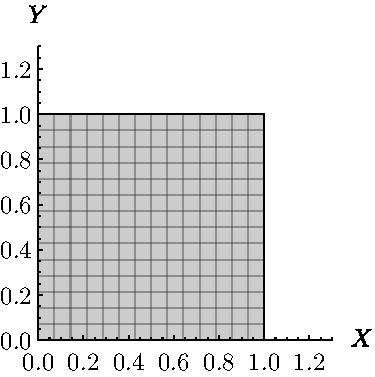
\includegraphics[width=0.4\textwidth]{images/gibanje0.pdf}
    \hspace{1em}
    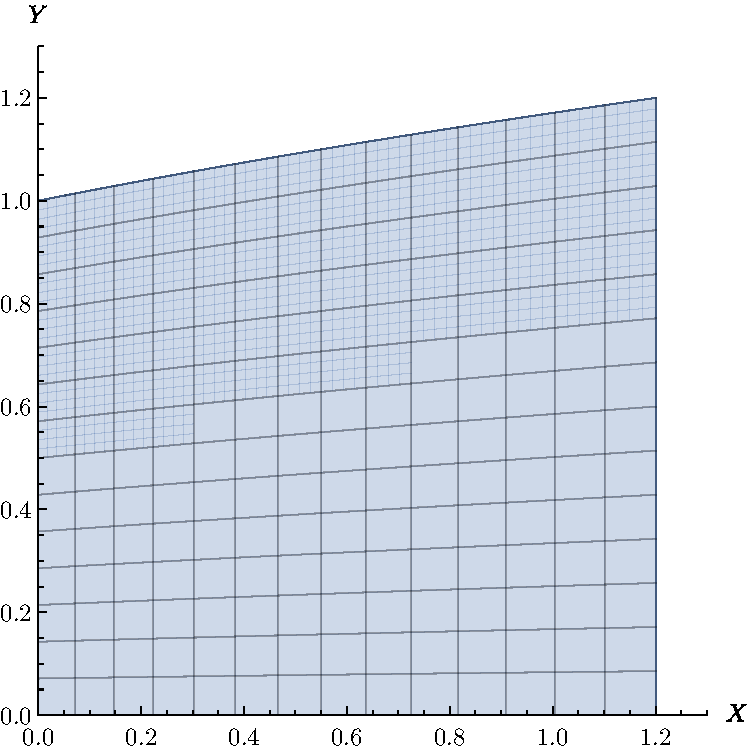
\includegraphics[width=0.4\textwidth]{images/gibanje02.pdf}
    \caption[Primer gibanja enotske kocke.]{Prerez enotske kocke pri $Z = 0$ v referenčni
      konfiguraciji (levo) in v prostorski konfiguraciji ob času $t=0.2$ (desno).}
    \label{fig:gibanje}
  \end{figure}
  Za vsak $t\geq 0$ je $\vx$ difeomorfizem, saj velja
  \begin{equation}
    \det\left( \dpar{\vx}{(X, Y, Z)} \right) = (1+tX)(1+2tX) > 0.
  \end{equation}
  Zato lahko izrazimo obratno preslikavo
  \begin{equation}
    \vX(t, x, y, z) = \left(\frac{\sqrt{4 t x+1}-1}{2 t}, \frac{y
    \left(\sqrt{4 t x+1}-1\right)}{2 t x}, z\right).
    \label{eq:gibanje-inv}
  \end{equation}
\end{primer}

Vsako količino $\phi$, definirano na telesu $\B$, kot na primer temperaturo ali hitrost, lahko
zapišemo na dva načina, v prostorskem ali v referenčnem položaju. Za funkcijo
\begin{align}
  \tilde \phi\colon B &\to \phi(\B) \nonumber \\
  \vX&\mapsto \phi(\chi_R^{-1}(\vX)), \label{eq:toref}
\end{align}
pravimo, da je zapisana v referenčnem položaju in pišemo $\tilde\phi =
\phi(\vX)$.
Podobno za funkcijo
\begin{align}
  \hat \phi\colon B_t &\to \phi(\B) \nonumber \\
  \vx&\mapsto \phi(\chi_t^{-1}(\vx)), \label{eq:topro}
\end{align}
pravimo, da je zapisana v prostorskem položaju in pišemo $\hat\phi = \phi(\vx)$.
Med obema zapisoma lahko prehajamo s pomočjo zveze~\eqref{eq:pros-ref} ali njenega inverza kot
$\phi(\vx) = \phi(\vx(t, \vX))$ ali $\phi(\vX) = \phi(\vX(\vx, t))$.

Podoben zapis bomo uporabljali tudi pri diferencialnih operatorjih. Pri odvodih
moramo povedati, ali na količino gledamo v prostorskem ali v referenčnem
položaju. Z velikimi črkami bomo pisali operatorje, kjer odvajamo glede na
referenčni položaj, z malimi pa tiste, kjer odvajamo glede na prostorskega.

\begin{primer}
  Dano imamo količino $\vartheta(t, X, Y, Z) = tX^2 + 2 ZY$, ki je zapisana v
  referenčnem položaju. Če jo zapišemo v prostorskih s pomočjo izpeljane
  inverzne relacije~\eqref{eq:gibanje-inv} iz primera~\ref{prim:gib}, dobimo
  \[
    \vartheta(t, x, y, z) = \frac{2 t x^2+2 y z \left(\sqrt{4 t x+1}-1\right)-x
    \sqrt{4 t x+1}+x}{2 t x}.
  \]
  Demonstrirajmo še uporabo diferencialnih operatorjev, izračunajmo
  \begin{align}
    \dpar{\vartheta}{Y} &= 2Z  \\
    \dpar{\vartheta}{y} &= \frac{z \left(\sqrt{4 t x+1}-1\right)}{t x}.
  \end{align}
  Te odvode bi zopet lahko zapisali kot funkcije referenčnega ali prostorskega položaja. Podobno se
  obnašajo časovni odvodi.
  \begin{align}
    \DDt{} \vartheta &= X^2 \\
    \ddt{} \vartheta &=  -\frac{\left(-2 t x+\sqrt{4 t x+1}-1\right) (x-2 y
    z)}{2 t^2 x \sqrt{4 t x+1}}.
  \end{align}
  Zapis $\DDt \vartheta(t, x, y, z)$ predstavlja torej časovni odvod $\vartheta$, pri konstantnem
  referenčnem položaju, zapisan v prostorski konfiguraciji. Izračunamo ga tako, da izraz prevedemo
  v referenčni položaj, odvajamo po času in prenesemo nazaj v prostorsko konfiguracijo. S simboli
  lahko to zapišemo kot
  \begin{equation}
    \left(\DDt{} \vartheta\right)(t, \vx) = \left( \DDt{}\vartheta(\vx(t, \vX))
    \right)(\vX(t, \vx)).
  \end{equation}
\end{primer}

Definirajmo še osnovne pojme pomika, hitrosti in pospeška.
\begin{definicija}
  Količino \begin{equation} \vu(\vX) = \vx(t, \vX) - \vX \end{equation} imenujemo \emph{pomik}.
  Količino \begin{equation} \vv(\vX) = \DDt{\vx}(t, \vX) \end{equation} imenujemo \emph{hitrost}.
  Količino \begin{equation} \va(\vX) = \DDt{\vv}(t, \vX) \end{equation} imenujemo \emph{pospešek}.
\end{definicija}
\begin{trditev}
  Odvod po času v referenčnem koordinatnem sistemu se lahko direktno izračuna v
  prostorskem kot
  \begin{equation}
    \DDt{\phi}(t, \vx) = \ddt{\phi}(t, \vx) + ((\grad \phi)(t, \vx)) \vv(t, \vx).
  \end{equation}
  Pri tem je $\phi$ skalarna, vektorska ali tenzorska količina.
\end{trditev}
\begin{proof}
  Po definiciji najprej prenesemo $\phi$ v referenčni koordinatni sistem z
  uporabo~\ref{eq:toref}. Nato odvajamo po verižnem pravilu
  \begin{align*}
    \DDt \phi(t, \vx) &= \DDt \phi(t, \vx(t, \vX)) =
    \ddt \phi(t, \vx) + \dpar{\phi}{\vx} \DDt{\vx} (t, \vX) = \\ \nonumber
    &= \ddt \phi(t, \vx) + ((\grad \phi)(t, \vx)) \vv(t, \vX(\vx, t)). \qedhere
  \end{align*}
\end{proof}

Poleg že naštetih količin pa imajo telesa tudi druge fizikalne lastnosti, kot so
masa in volumen, ki vplivajo na gibanje. Za modeliranje teh si pomagamo z
merami.

\begin{definicija}
  Predpostavimo, da imamo na $\B$ definirani dve $\sigma$-končni meri, $m$ in $V$, ki nam
  predstavljata maso in volumen. Predpostavimo še, da je $m$ absolutno zvezna glede na $V$, torej,
  če je volumen nekega podtelesa nič, je tudi njegova masa nič. Od tod po Radon-Nikodymovem izreku
  sledi, da obstaja merljiva funkcija $\rho =
  \dd{m}{V}$, da velja
  \begin{equation}
    m(A) = \int_{A} \rho dV
  \end{equation}
  za vsako merljivo podmnožico $A \subseteq \B$.
  Funkciji $\rho\colon\B\to[0, \infty)$ pravimo \emph{gostota}.
\end{definicija}
\begin{opomba}
  Ponavadi za $V$ vzamemo kar Lebesgueovo mero na $\R^3$, mero $m$ pa podamo tako, da
  podamo gostoto telesa $\rho$. Meri $m$ in $V$ s potiskom prek konfiguracij
  razširimo na referenčni in prostorski položaj.
\end{opomba}

\subsubsection{Aksiomi gibanja}
Iz mehanike točke in iz klasične mehanike vemo, da gibanje zadošča nekim
zakonom, ki jih bomo za nadaljnje izpeljave privzeli kot aksiome.

\begin{definicija}
  Množica $\B' \subseteq \B$ je \emph{podtelo} telesa $\B$, če je sama telo za isto družino
  konfiguracij.
\end{definicija}

\begin{aksiom}[Zakon o ohranitvi mase]
  \label{aks:masa}
  Za vsako podtelo $\B' \subseteq  \B$ in vsako njegovo gibanje velja
  \begin{equation}
  \DDt{}m(B_t') = 0.
    \label{eq:masa}
  \end{equation}
  Masa se med gibanjem niti ne izgublja niti ne nastaja in je vseskozi konstantna.
\end{aksiom}

Druga dva aksioma bosta poleg mase imela opraviti s silami. Kako lahko sile delujejo na telo?  En
način so sile na daljavo, kot na primer gravitacija, ki delujejo na vsak košček telesa posebej.
Drug način so kontaktne sile, ki nastanejo zaradi stika med telesi in se prenašajo preko površine.
Sile v skladu s hipotezo kontinuuma opišemo z njihovimi \emph{gostotami} in vedno delujejo na
telo v njegovi prostorski konfiguraciji, saj je to konfiguracija, ki jo telo dejansko zavzame med
gibanjem. Če je sila konstantna, potem gostota sile predstavlja silo na enoto volumna ali
površine, kar pogosto imenujemo \emph{tlak}.

\begin{definicija}
  \emph{Volumenska gostota sile} $\vf$ je zvezna družina zveznih funkcij
  \begin{equation}
    \vf_t\colon B_t\to\R^3.
  \end{equation}
\end{definicija}
\begin{definicija}
  \emph{Površinska gostota sile} $\vt$ je zvezna družina zveznih funkcij
  \begin{equation}
   \vt_t\colon\partial B_t\to\R^3.
  \end{equation}
\end{definicija}
\begin{opomba}
  Zveznost družine funkcij podobno kot v definiciji~\ref{def:gibanje} pomeni, da je
  funkcija
  \begin{align*}
    \vf\colon \R \times B \subseteq \R \times \R^3 &\to \R^3 \\
    (t, \vX) &\mapsto \vf_t(\vx(t, \vX))
  \end{align*}
  zvezna kot funkcija iz $\R^4$ v $\R^3$. Poenostavljeno pišemo $\vf$ in $\vt$ kar kot funkciji
  odvisni od $t$ in $\vx$, torej $\vf = \vf(t, \vx)$ in $\vt = \vt(t, \vx)$.
\end{opomba}
\begin{primer}
  Gostota gravitacijske sile je enaka $\vf = \rho \vec{g}$, kjer je $\vec{g}$ gravitacijski
  pospešek in je neodvisna od časa in položaja.
\end{primer}

\begin{aksiom}[Zakon o ohranitvi gibalne količine]
  \label{aks:gib}
  Za vsako podtelo $\B' \subseteq \B$ velja
  \begin{equation}
    \DDt{}\int_{B_t'} \vv dm = \int_{B_t'} \vf dV + \int_{\partial B_t'} \vec t dS.
    \label{eq:gib}
  \end{equation}
  Sprememba gibalne količine je enaka vsoti vseh sil, ki delujejo na telo.
\end{aksiom}

\begin{aksiom}[Zakon o ohranitvi vrtilne količine]
  \label{aks:vrt}
  Za vsako podtelo $\B' \subseteq \B$ velja
  \begin{equation}
    \DDt{}\int_{B_t'}\vx \times \vv dm = \int_{B_t'} \vx \times \vf dV +
    \int_{\partial B_t'} \vx\times\vt dS.
    \label{eq:vrt}
  \end{equation}
  Sprememba vrtilne količine je enaka vsoti vseh zunanjih navorov, ki delujejo
  na telo.
\end{aksiom}
\begin{opomba}
  Pri aksiomu~\ref{aks:vrt} smo predpostavili, da na kontinuum ne delujejo notranji navori, ampak da
  so vsi navori posledica delovanja zunanjih sil. Drugače povedano, predpostavili smo
  \emph{nepolarnost} kontinuuma.
\end{opomba}

V vseh treh aksiomih nastopa odvod po času v referenčni konfiguraciji nekega
integrala, zapisanega v prostorski konfiguraciji. Tu ne velja običajen izrek o
odvajanju pod integralom, zato moramo izraz pod integralom najprej prenesti v
referenčni položaj, zamenjati odvod in integral, nato pa ga prenesti nazaj.
Naredimo to najprej za aksiom o ohranitvi mase.
\begin{trditev} Masa se ohranja $(\DDt{}m(B_t) = 0)$ natanko tedaj, ko je
  \begin{equation}
    \DDt\rho + \rho\div\vv = 0.
    \label{eq:ohr-masa}
  \end{equation}
\end{trditev}
\begin{proof}
Trditev pokaže direkten račun, kjer bomo zamenjali integralsko spremenljivko iz
$\vx$ na $\vX$ in nato nazaj. Pri uvedbi nove spremenljivke se bo v integralu
pojavila determinanta $J = \det(F)$ diferenciala prehodne preslikave $F =
\dpar{\vx}{\vX}$, prav tako pa tudi njen odvod $\DDt{J}$, zato ga izračunajmo vnaprej:
\begin{align*}
  \DDt J &= \tr\left(\operatorname{adj}(F) \DDt{F}\right) =
  \tr\left(\det(F)F^{-1} \dpar{^2\vx}{\vX\partial t}\right) =
  \det(F)\tr\left(\dpar{\vv}{\vX}F^{-1}\right) = \\ &=
  \det(F)\tr\left(\dpar{\vv}{\vX}\dpar{\vX}{\vx}\right) =
  \det(F)\tr\left(\grad \vv\right) =
  \det(F)\div \vv.
\end{align*}
Pri tem smo uporabili Jacobijevo formulo za računanje odvoda
determinante, ciklično lastnost sledi, formulo za računanje odvoda inverza in verižno pravilo.
Sedaj imamo vse pripravljeno za glavni izračun.
\begin{align*}
  0 &= \DDt{}m(B_t) =
  \DDt{} \int_{B_t} dm =
  \DDt{} \int_{B_t} \rho dV =
  \DDt{} \int_{B} \rho J dV =\\ &=
  \int_{B} \DDt{}(\rho J) dV =
  \int_{B}\left( \DDt{\rho} J + \rho \DDt{J} \right)dV = \\ &=
  \int_{B}\left( \DDt{\rho}  + \rho \div\vv\right) J dV =
  \int_{B_t}\left( \DDt{\rho}  + \rho \div\vv\right) dV.
\end{align*}
Ker je integral nič za vsako telo, mora biti nujno integrand nič, in obratno, če
je integrand nič, se masa ohranja.
\end{proof}

Zgornjo trditev bomo s pridom uporabili pri izračunu odvoda integrala splošne
količine.
\begin{trditev}
  \label{trd:swap-der-int}
  Naj bo $\phi$ neka skalarna, vektorska ali tenzorska količina in privzemimo aksiom o ohranitvi
  mase. Potem velja
  \begin{equation}
    \DDt{} \int_{B_t}\phi dm = \int_{B_t} \DDt{\phi} dm.
    \label{eq:swap-der-int}
  \end{equation}
\end{trditev}
\begin{proof}
Postopamo enako kot v prejšnji trditvi. Izračunamo
\begin{align*}
    \DDt{} \int_{B_t}\phi dm &=
    \DDt{} \int_{B}\phi \rho J dV =
    \int_{B} \DDt{(\phi \rho J)} dV  = \\ &=
  \int_{B} \left(\DDt{\phi} \rho J + \phi \left(\underbrace{\DDt{\rho} + \rho
  \div \vv}_{=\;0 \text{ po \eqref{eq:ohr-masa}}} \right) \right)dV  = \\ &=
  \int_{B} \DDt{\phi} \rho JdV =
  \int_{B_t} \DDt{\phi} dm. \qedhere
\end{align*}
\end{proof}

\subsection{Napetostni tenzor}
Predstavljajmo si, da na telo deluje neka površinska sila z gostoto $\vt$. Ta sila deluje na zunanjo
površino telesa, nato pa se prenaša skozi telo od točke do točke. V telesu si zamislimo neko podtelo.
Na površini tega podtelesa zunanji del kontinuuma deluje na podtelo, toda ekvivalentno bi bilo, če
bi zunanji del odstranili in na površino preostanka delovali z enakim poljem sil, kot je prej
deloval zunanji del.

Ta razmislek nam ponuja naslednji opis notranjih in površinskih sil telesa. V nekem trenutku $t$
se postavimo v neko točko $\vx$ v telesu in si zamislimo neko podtelo, tako da je izbrana točka
na njegovi površini. Tedaj obstaja vektor $\vt$, ki predstavlja silo, s katero preostali kontinuum
deluje v tej točki na izbrano podtelo. Če bi si izbrali drugo podtelo, bi bila v splošnem sila
drugačna. Toda, če sta imeli dve podtelesi v tisti točki enako zunanjo enotsko normalo $\vn$ na
površino  in posledično enako tangentno ravnino v tisti točki, bo vektor $\vt$ še vedno enak, saj
bosta lokalno telesi izgledali enaki. Vektor $\vt$ je torej odvisen od izbrane točke, trenutka v
času, ko ga opazujemo in normale na izbrano površino podtelesa, ter ničesar drugega; neodvisen je na
primer od ukrivljenosti ploskve v tisti točki. Temu razmisleku se reče \emph{Cauchyjeva hipoteza}.

\begin{aksiom}[Cauchyjeva hipoteza]
  V telesu obstaja vektorsko polje $\vt$ inducirano s površinskimi silami, ki
  je odvisno samo od položaja, časa in normale na površino (resnično ali
  namišljeno), kjer ga opazujemo. S simboli lahko zapišemo
  \begin{equation}
    \vt = \vt(t, \vx, \vn).
  \end{equation}
\end{aksiom}

Iz zgornjega razmisleka se zdi, da bi morala biti sila, s katero prvi del
kontinuuma deluje na drugega, nasprotno enaka sili, s katero drugi deluje na
prvega. Temu se reče tudi tretji Newtonov zakon za mehaniko kontinuuma in
ga ni treba privzeti kot aksiom, ampak lahko dokažemo iz do sedaj
privzetih aksiomov. Dokaza tega in naslednjega izreka sta povzeta po dokazih
iz~\cite[str.\ 104--107]{hjelmstad2007fundamentals}.
\begin{trditev}[Cauchyjeva recipročna relacija]
  \label{trd:cauchy-reciprocal}
  \begin{equation}
    \vt(t, \vx, -\vn) = -\vt(t, \vx, \vn).
    \label{eq:cauchy-reciprocal}
  \end{equation}
\end{trditev}
\begin{proof}
Izberimo trenutek v času $t$ in točko $\vx$. Krajše pišimo $\vt_{\vn} = \vt(t, \vx,
\vn)$. Oglejmo si podtelo v obliki krožnega valja z višino $h^2$ in radijem $h$, ki ima
v središču točko $\vx$ in je $\vn$ normala na eno izmed osnovnic.
Tako podtelo zaradi odprtosti $\B$ gotovo obstaja za dovolj majhen $h$. Označimo
osnovnico z normalo $\vn$ z $B^+$, nasprotno z $B^-$ in plašč s $P$. Površina
vsake osnovnice je $\pi h^2$, površina plašča pa $2 \pi h^3$. Volumen valja je
$\pi h^4$. Primer valja je prikazan na sliki~\ref{fig:valj}.

\begin{figure}[h]
  \centering
  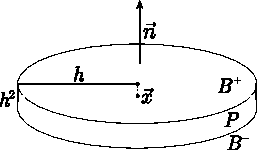
\includegraphics[width=0.3\textwidth]{images/cauchy_disc.pdf}
  \caption{Valj, uporabljen v dokazu Cauchyjeve recipročne relacije.}
  \label{fig:valj}
\end{figure}

Uporabimo za ta
valj aksiom o gibalni količini~\eqref{eq:gib}:
\[  \DDt{} \int_{B_t} \vv dm = \int_{B_t} \vf dV + \int_{\partial B_t} \vt dS. \]
Po trditvi~\ref{trd:swap-der-int} lahko zamenjamo odvod in integral, rob valja
razpišimo po ploskvah:
\[
  \int_{B_t} \DDt{\vv} \rho dV = \int_{B_t} \vf dV + \int_{B^+} \vt_{\vn} dS +
  \int_{B^-}\vt_{-\vn} dS + \int_{P} \vt_{\vm(\vx)}dS.
\]
Vektor $\vm(\vx)$ pri tem označuje normalo na plašč valja. Celotno enačbo pomnožimo s konstantnim
vektorjem $\vc$ in na vsakem od integralov, ki so postali integrali skalarnih funkcij, uporabimo izrek
o povprečni vrednosti
\begin{align*}
  V(B) (\rho\DDt{\vv})(\vx_1)\cdot\vc = V(B) \vf(\vx_2)\cdot\vc &+ S(B^+)\vt_{\vn}(\vx_3)\cdot\vc\;+ \\&+
  S(B^-)\vt_{-\vn}(\vx_4)\cdot\vc + S(P)\vt_{\vm(\vx)}(\vx_5)\cdot\vc,
\end{align*}
kjer so $\vx_1, \vx_2, \vx_3, \vx_4, \vx_5$ neke vmesne točke v ali na površini valja.
Če vstavimo izraze za volumen in površine ploskev dobimo
\[
  \pi h^4 (\rho \DDt{\vv})(\vx_1)\cdot\vc = \left[\pi h^4 \vf(\vx_2) + \pi h^2 \vt_{\vn}(\vx_3) +
  \pi h^2 \vt_{-\vn}(\vx_4) + 2 \pi h^3 \vt_{\vm(x)}(\vx_5)\right]\cdot\vc.
\]
Celoten izraz delimo z $\pi h^2$ in pogledamo limito $h\to 0$, gredo vse točke
$\vx_i$ proti $\vx$ in dobimo
\[
  0 = (\vt_{\vn}(\vx) + \vt_{-\vn}(\vx))\cdot\vc.
\]
Ker zgornja enakost velja za poljuben vektor $\vc$, velja tudi
\[
  0 = (\vt_{\vn}(\vx) + \vt_{-\vn}(\vx)),
\]
kar je točno to, kar smo želeli pokazati.
\end{proof}

Izkaže se, da velja še več, in sicer da je vektor $\vt$ linearno odvisen od normale. S pomočjo
prejšnje trditve lahko pokažemo naslednji izrek, ki nam da na voljo matematični objekt, s pomočjo
katerega opišemo napetost v materialu.
\begin{izrek}[Cauchyjev izrek o napetosti]
  Obstaja tenzor $\ts$, tako da velja
  \begin{equation}
    \vt(t, \vx, \vn) = \ts(t, \vx)\vn.
  \end{equation}
  Tenzor $\ts$ se imenuje Cauchyjev napetostni tenzor.
\end{izrek}
\begin{proof}
Podobno kot pri Cauchyjevi recipročni relaciji si tokrat izberimo majhno telo z ogliščem v točki
$\vx$. Naj bo to tetraeder s tremi stranicami, vzporednimi koordinatnim osem in normalo $\vn$ na
ploskev, ki jo razpenjajo preostale tri stranice, kot prikazano na sliki~\ref{fig:tetra}.

\begin{figure}[h]
  \centering
  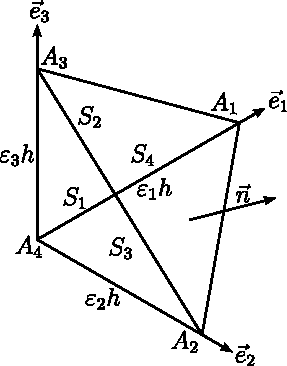
\includegraphics[width=0.3\textwidth]{images/cauchy_tetrahedron.pdf}
  \caption{Tetraeder, uporabljen v dokazu Cauchyjevega izreka o napetosti.}
  \label{fig:tetra}
\end{figure}

Označimo oglišča tetraedra z $A_1, A_2, A_3, A_4 = \vx$ in ploskev nasproti izbranega oglišča s
$S_1, S_2, S_3, S_4$. Ploščine teh ploskev označimo z $a_1, a_2, a_3, a_4$. Naj bodo pravokotne
stranice tetraedra dolge $\eps_1 h$, $\eps_2 h$ in $\eps_3 h$, kjer razmerje $\eps_1 : \eps_2 :
\eps_3$ določimo tako, da je normala na $S_4$ enaka $\vn$. Opisana konfiguracija je prikazana na
sliki~\ref{fig:tetra}. Izračunamo lahko ploščine ploskev $a_1 = \frac12 \eps_2\eps_3h^2$,
$a_2 = \frac12 \eps_1\eps_3h^2$ in $a_3 = \frac12 \eps_1\eps_2h^2$. Volumen tetraedra je $V =
\frac16 \eps_1\eps_2\eps_3h^3$. Vektorje v smeri koordinatnih osi standardno označimo z $\ei$,
$\ej$, $\ek$. Zunanja normala na ploskev $S_1$ je $-\ei$, na ploskev $S_2$ je $-\ej$ in na ploskev
$S_3$ je $-\ek$. Normalo na preostalo ploskev, ki bo dolga ravno toliko, kot je ploščina te ploskve,
dobimo s pomočjo vektorskega produkta stranic, ki jo oklepata.
\begin{align*}
  a_4\vn &= \frac12 (\eps_1h \ei - \eps_2h \ej) \times (\eps_3h \ek - \eps_2h
  \ej) = \\ &=
  -\frac12 \eps_2\eps_3 h^2\ei
  -\frac12 \eps_1\eps_3 h^2\ej
  -\frac12 \eps_1\eps_2 h^2\ek = \\
  &= a_1 \ei + a_2 \ej + a_3 \ek.
\end{align*}
Če to pomnožimo z $i$-tim baznim vektorjem, dobimo $a_i = (\vn\cdot\vec{e}_i)
a_4$.
Zopet uporabimo aksiom~\ref{aks:gib} o ohranitvi gibalne količine, razpišemo integral po površini
tetraedra po posameznih ploskvah, pomnožimo izraz s konstantnim vektorjem $\vc$ in nato uporabimo
izrek o povprečni vrednosti, ter dobimo
\begin{align*}
  \DDt{} \int_{B_t} \vv dm &= \int_{B_t} \vf dV + \int_{\partial {B_t}} \vt dS \\
\int_{B_t} \rho\DDt{\vv} dV &= \int_{B_t} \vf dV +
  \int_{S_1} \vt_{-\ei} dS +
  \int_{S_2} \vt_{-\ej} dS +
  \int_{S_3} \vt_{-\ek} dS +
  \int_{S_4} \vt_{\vn} dS
  \\
  V (\rho\DDt{\vv})(\vx_1)\cdot\vc &= \left[V \vf(\vx_2) +
  a_1 \vt_{-\ei}(\vx_3) + a_2 \vt_{-\ej}(\vx_4) + a_3 \vt_{-\ek}(\vx_5) + a_4
\vt_{\vn}(\vx_6)\right]\cdot \vc,
\end{align*}
pri čemer so $\vx_i$, kot v prejšnjem dokazu, neke točke v notranjosti ali na
površini tetraedra. Sedaj enačbo delimo z $a_4$ in pošljemo limito $h \to 0$.
Vse točke $\vx_i$ limitirajo proti $\vx$, člena, ki vsebujeta volumen tetraedra,
pa se približujeta 0. Z upoštevanjem
\[
  \lim_{h\to0} \frac{a_i}{a_4} = \lim_{h\to0}\frac{(\vn\cdot\vec{e}_i) a_4}{a_4}
  = \vn\cdot\vec{e}_i
\]
dobimo
\[
  0 = \left[\vt_{\vn} + \sum_{i=1}^3 (\vn \cdot\vec{e}_i) \vt_{-\vec{e}_i}\right]\vc.
\]
Zgornja enakost velja za vsak vektor $\vc$ in ko uporabimo še Cauchyjevo recipročno
relacijo~\eqref{eq:cauchy-reciprocal}, dobimo
\[
  \vt_{\vn} = \sum_{i=1}^3 (\vn \cdot\vec{e}_i) \vt_{\vec{e}_i}.
\]
Ta zveza nam pove, kako je napetost na poljubni ploskvi povezana z napetostmi na koordinatnih
ploskvah. To nam dovoljuje definicijo \emph{Cauchyjevega napetostnega tenzorja}
$\ts$
\[
  \ts = \sum_{i=1}^3 \vt_{\vec{e}_i}\otimes \vec{e}_i,
\]
za katerega res velja
\[
  \ts\vn = \sum_{i=1}^3 (\vt_{\vec{e}_i}\otimes \vec{e}_i)(\vn) =
  \sum_{i=1}^3 (\vn \cdot\vec{e}_i) \vt_{\vec{e}_i} = \vt_{\vn}. \qedhere
\]
\end{proof}

\subsection{Enačbe gibanja}
V tem razdelku bomo iz aksiomov izpeljali lokalne enačbe gibanja, tako da jih
bomo iz integralske oblike prevedli v diferencialno.
Prevedimo najprej aksiom~\ref{aks:gib} o ohranitvi gibalne količine.
\begin{izrek}[Cauchyjeva momentna enačba]
  Za gibanje kontinuuma velja Cauchyjeva momentna enačba
  \begin{equation}
    \rho \DDt{\vv} = \vf + \div \sigma.
    \label{eq:cauchy-moment}
  \end{equation}
\end{izrek}
\begin{opomba}
  Tako kot je enačba~\eqref{eq:cauchy-reciprocal} analogija tretjega Newtonovega zakona, je
  enačba~\eqref{eq:cauchy-moment} analogija drugega Newtonovega zakona: na levi imamo produkt
  gostote mase in pospeška, na desni pa gostoto vseh sil, ki delujejo na telo.
\end{opomba}
\begin{proof}
Za vsako telo s prostorsko konfiguracijo $B_t$ velja
\begin{align*}
  \DDt{} \int_{B_t} \vv dm &= \int_{B_t} \vf dV + \int_{\partial {B_t}} \vt dS \\
  \int_{B_t} \DDt{\vv}\rho dV &= \int_{B_t} \vf dV + \int_{\partial {B_t}} \ts \vn dS \\
  \int_{B_t} \DDt{\vv}\rho dV &= \int_{B_t} \vf dV + \int_{B_t} \div \ts dV \\
  0 &= \int_{B_t}\left(\DDt{\vv}\rho - \vf - \div \ts\right) dV.
\end{align*}
V računu smo uporabili Gaussov izrek~\ref{izr:gauss} za tenzorje drugega reda in
izrek~\ref{trd:swap-der-int} o menjavi odvoda in integrala. Ker mora biti zadnji
integral nič za vsako telo, mora biti integrand nič, kar dokaže našo enačbo.
\end{proof}

Do sedaj še nismo uporabili aksioma~\ref{aks:vrt} o vrtilni količini.
Njegova lokalna oblika se prevede na zelo enostavno trditev o simetriji
Cauchyjevega napetostnega tenzorja.
\begin{trditev}
  \label{trd:sigma-symmetric}
  Cauchyjev napetostni tenzor je simetričen:
  \begin{equation}
    \ts^\T = \ts.
  \end{equation}
\end{trditev}
\begin{proof}
Začnimo z zakonom o vrtilni količini~\eqref{eq:vrt} in ga prevedimo v lokalno
obliko.
\begin{equation}
  \DDt{}\int_{B_t}\vx \times \vv dm = \int_{B_t} \vx \times \vf dV +
  \int_{\partial B_t} \vx\times\vt dS.
\end{equation}
Posvetimo se zadnjemu členu in ga pomnožimo s konstantnim vektorjem $\vw$:
\begin{align*}
\left(\int_{\partial B_t} \vx \times \vt dS\right)\cdot \vw  &=
  \int_{\partial B_t} \langle \vx, \vt, \vw \rangle dS =
  \int_{\partial B_t} \langle \vw, \vx, \vt \rangle dS = \\ &=
  \int_{\partial B_t} (\vw \times \vx) \cdot \vt dS =
  \int_{\partial B_t} (\vw \times \vx) \cdot \ts\vn dS = \\ &=
  \int_{\partial B_t} \ts^\T(\vw \times \vx) \cdot d\vec{S} =
  \int_{B_t} \div (\ts^\T(\vw \times \vx)) dV = \\ &=
\int_{B_t} [\langle \div \ts, \vw, \vx\rangle +  \ts : \grad (\vw \times \vx)] dV.
\end{align*}
Zgoraj smo uporabili po vrsti: definicijo in cikličnost mešanega produkta, definicijo
$\ts^\T\!$, Gaussov izrek in relacijo iz trditve~\ref{trd:div-tv}.

Podobno z $\vw$ pomnožimo tudi zakon o vrtilni količini in vstavimo zgornjo
relacijo.
\begin{align*}
  0 &= \left(\DDt{}\int_{B_t}\vx \times \vv dm - \int_{B_t} \vx \times \vf dV -
  \int_{\partial B_t} \vx\times\vt dS\right)\cdot \vw = \\ &=
  \DDt{}\int_{B_t}\langle \vx, \vv, \vw\rangle  dm - \int_{B_t} \langle \vx,
  \vf, \vw\rangle dV - \int_{B_t} [\langle \div \ts, \vw, \vx\rangle +  \ts :
  \grad (\vw \times \vx)] dV = \\ &=
  \int_{B_t}\langle \rho \DDt\vv, \vw, \vx \rangle  dV - \int_{B_t} \langle \vf,
  \vw, \vx\rangle dV - \int_{B_t} [\langle \div \ts, \vw, \vx\rangle +  \ts :
  \grad (\vw \times \vx)] dV = \\ &=
\int_{B_t}\left[ \left\langle\rho \DDt\vv - \vf - \div \ts, \vw, \vx\right\rangle -  \ts : \grad
  (\vw \times \vx)\right] dV = \\ &=
- \int_{B_t} \ts : \grad (\vw \times \vx) dV.
\end{align*}
Uporabili smo definicijo in cikličnost mešanega produkta, Cauchyjevo momentno
enačbo~\eqref{eq:cauchy-moment} in dejstvo, da je
\[
  \DDt{}\langle \vx, \vv, \vw \rangle =
  \langle \vv, \vv, \vw \rangle +
  \langle \vx, \DDt\vv, \vw \rangle =
  \langle \DDt\vv, \vw, \vx \rangle.
\]
Ker aksiom o vrtilni količini drži za vsako telo, mora biti
\[
  \ts : \grad (\vw \times \vx) = 0,
\]
za poljuben vektor $\vw$. Tenzor $\grad (\vw \times \vx)$ je antisimetričen in
vsak antisimetričen tenzor lahko s pomočjo njegovega osnega vektorja zapišemo v
tej obliki, zato je zgornja relacija ekvivalentna trditvi, da je
\[ \ts : w = 0\] za vsak antisimetričen tenzor $w$.
Torej je $\ts \in Asym(\R^3)^\perp$ in po trditvi~\ref{trd:dot-antisym-tensor}
mora biti $\ts$ simetričen.
\end{proof}

\subsection{Konstitutivne enačbe}
Do sedaj izpeljane enačbe veljajo za poljuben kontinuum, naj bo to tekočina, plastična ali elastična
trdnina. V tem razdelku si bomo ogledali enačbe, ki definirajo obnašanje našega kontinuuma kot
elastične trdnine preko posplošitve Hookovega zakona, ki povezuje napetosti v materialu z njegovo
deformacijo. Naučili smo se že, kako izražamo napetost, sedaj pa si poglejmo, kako merimo
deformacijo teles. Tukaj bomo tudi privzeli, da je referenčna konfiguracija kar prostorska
konfiguracija na začetku gibanja.

\subsubsection{Mera deformacije}
\begin{definicija}[Gradient deformacije]
  Količino $F = \dpar{\vx}{\vX}(t, \vX) = \Grad \vx$ imenujemo \emph{gradient
  deformacije}.
\end{definicija}

Tenzor $F$ je drugega reda in nam v vsaki točki predstavlja lokalno deformacijo
telesa. Privzeli smo že, da je $\vx$ difeomorfizem, torej je $F$ neizrojen,
dodatno pa bomo privzeli še, da gibanje $\vx$ \emph{ohranja orientacijo}, saj
so taka vsa gibanja v realnosti. Od tod sledi, da je $\det F > 0$.
Fizikalno interpretacijo $F$ dobimo z naslednjim Taylorjevim razvojem:
\begin{equation}
   d\vx := \vx(t, \vX+d\vX) - \vx(t, \vX) = F d\vX + O(d\vX^2).
\end{equation}
Tenzor $F$ do prvega reda natančno opiše kako se vektor $d\vX$ iz referenčne
konfiguracije deformira v vektor $d\vx$ v prostorski konfiguraciji.

Vendar, ni vsa deformacija, ki jo opiše tenzor $F$ taka, da bi povzročala
napetosti. Hookov zakon v eni dimenziji pravi, da je sila sorazmerna raztezku.
Če imamo opravka s togim premikom $\vX \mapsto Q\vX + a$, ta premik ne bo povzročil
nobene napetosti, saj se bo telo samo premaknilo, ne pa raztegnilo.

\begin{primer}
Naj bo dana tanka palica kot na sliki~\ref{fig:palica}, ki jo raztegnemo vzdolž
njene nosilke.
\begin{figure}[h]
  \centering
  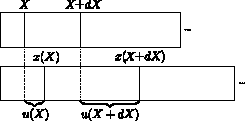
\includegraphics[width=0.55\textwidth]{images/stretch1d.pdf}
  \caption{Razteg tanke palice vzdolž njene osi.}
  \label{fig:palica}
\end{figure}
Premik v točki $\vX$ je $\vu(\vX) = \vx - \vX$, v točki $\vX+d\vX$ pa $u(\vX+d\vX)$.
Dejanski relativni raztezek delčka palice dolžine $d\vX$ pa je
\begin{align}
  \frac{d\vx - d\vX}{d\vX} &= \frac{\vx(\vX+d\vX) - \vx(\vX) - (\vX + d\vX - \vX)}{d\vX} = \nonumber \\ &=
  \frac{\vu(\vX + d\vX) - \vu(\vX)}{d\vX} = \vu\,'(\vX) + O(d\vX).
\end{align}
Do prvega reda je relativni raztezek v točki $\vX$ enak kar $\vu\,'(\vX)$.

Preverimo še, da ta mera raztezka zadošča nekaterim intuitivnim zahtevam. Za
togi premik $\vX \mapsto \vX + c$ je $\vu(\vX) = c$ in $\vu\,'(\vX) \equiv 0$, kot
pričakovano.

Za enakomerni razteg $\vX \mapsto a\vX$ je $\vu(\vX) = a\vX - \vX$ in $\vu\,'(\vX) = a - 1$. Tudi
to ustreza pričakovanjem, saj za $a = 1$ ni raztezka, za $a< 1$ je to skrčitev
in je raztezek negativen, za $a>1$ pa dobimo pozitivno število.
\end{primer}

Posplošitev mere deformacije med točkama $\vX$ in $\vX+d\vX$ v višje dimenzije bi bila
\begin{equation}
   \eps_1 = \frac{\|d\vx\| - \|d\vX\|}{\|d\vX\|}.
\end{equation}
Toda veliko lažje je računati s kvadrati norm kot z normami vektorjev, zato je
bolj primerna Cauchyjeva mera
\begin{equation}
  \eps_2 = \frac{\|d\vx\|^2 - \|d\vX\|^2}{\|d\vX\|^2}.
\end{equation}
Ker velja $\eps_2 = (1+\eps_1)^2 - 1 = 2\eps_1 + \eps_1^2$, je za majhne pomike
$\eps_2 \approx 2\eps_1$. Meri sta za majhne pomike torej ekvivalentni.

Izračunajmo infinitezimalno aproksimacijo mere $\eps_2$.
\begin{align}
  \eps_2 &=
  \frac{\|d\vx\|^2 - \|d\vX\|^2}{\|d\vX\|^2} =
  \frac{\|d\vx\|^2}{\|d\vX\|^2}  - 1=
  \frac{\|F d\vX + O(d\vX^2)\|^2}{\|d\vX\|^2} - 1 = \nonumber \\ &=
  \frac{d\vX^\T F^\T F d\vX + O(d\vX^3)}{\|d\vX\|^2} - 1 =
  \frac{d\vX}{\|d\vX\|}(\underbrace{F^\T F - I}_{2E})\frac{d\vX}{\|d\vX\|} + O(d\vX)
\end{align}
V limiti $d\vX \to 0$ lahko mero $\eps_2$ predstavimo s tenzorjem $F^\T F- I$,
mero $\eps_1$ pa s tenzorjem $E$.

\begin{definicija}[deformacijski tenzor]
  Količina
  \begin{equation}
    E = \frac12 (F^\T F - I)
  \end{equation}
  se imenuje (Cauchy-Greenov) deformacijski tenzor.
\end{definicija}
\begin{trditev}
  Deformacijski tenzor $E$ lahko izrazimo z gradientom pomika kot
  \begin{equation}
    \label{eq:strain-tensor}
    E = \frac12\left( \Grad \vu + \Grad \vu^\T + \Grad \vu^\T \Grad \vu \right).
  \end{equation}
\end{trditev}
\begin{proof}
Trditev pokaže preprost račun. Spomnimo se, da je pomik definiran kot $\vu(\vX) =
\vx(\vX) - \vX$ in je gradient pomika enak
\[ \Grad \vu(\vX) = \dpar{\vu}{\vX} = \dpar{\vx}{\vX} - I = F - I. \]
Izračunamo:
\begin{align*}
  &\frac12\left( \Grad \vu + \Grad \vu^\T + \Grad \vu^\T \Grad \vu \right) = \\
  &\qquad=\frac12\left(F - I + F^\T - I  + (F-I)^\T(F-I)\right) = \\
  &\qquad=\frac12\left(F + F^T - 2I + F^\T F - F - F^T + I\right) = \\
  &\qquad=\frac12\left(F^\T F - I\right) = \\
  &\qquad=E.\qedhere
\end{align*}
\end{proof}

Deformacijo $F$ lahko s pomočjo polarnega razcepa zapišemo kot $F = RU$, kjer je
$R$ ortogonalna in $U$ pozitivno definitna matrika. Tenzor $R$ predstavlja
rotacijo, $U$ pa razteg in strig. Predstavljamo si lahko, da deformacijo $F$
izvedemo tako, da najprej telo v koordinatnem sistemu, v katerem je $U$ diagonalna,
raztegnemo, nato pa zavrtimo v končno lego.

Rotacija $R$ ne vpliva na obrabo in deformacijo materiala, saj je pomik tog in ne povzroča notranjih
napetosti. Prava mera deformacije, ki vpliva na napetost v materialu, torej ne vsebuje nobenih
rotacij. Za mero deformacije bi lahko vzeli kar razliko $U - I$, toda polarni razcep matrike je
težko izračunati. Poglejmo si kakšno zvezo ima zgoraj definirani deformacijski tenzor $E$ z $U$:
\begin{equation}
   E = \frac12(f^\T F - I) = \frac12(U^\T R^\T R U - I) = \frac12 (U^2 - I).
\end{equation}
Vidimo, da $E$ meri razliko $U^2 - I$, torej nam pove, kako se naše gibanje razlikuje od identitete,
ki predstavlja gibanje brez deformacij.

Kot pri enodimenzionalnem primeru si oglejmo, kako se $E$ obnaša pri enostavnih
deformacijah.
\begin{primer}
  Kot prej si oglejmo, da je za toge deformacije $E = 0$. Naj bo deformacija toga, torej oblike
  $\vX \mapsto Q\vX + c$ z ortogonalno konstantno matriko $Q$ in konstantnim $c$. Tedaj je
  \begin{equation}
     E = \frac12 (F^\T F - I) = \frac12(Q^\T Q - I) = \frac12(I - I) = 0.
  \end{equation}
  Oglejmo si še enostavni razteg v smeri osi, dan kot
  $\vX \mapsto \diag(\lambda_1, \lambda_2, \lambda_3) \vX$.
  V tem primeru velja $F = \diag(\lambda_1, \lambda_2, \lambda_3)$ in
  \begin{equation}
    E = \diag\left(
      \frac{\lambda_1^2-1}{2},
      \frac{\lambda_2^2-1}{2},
      \frac{\lambda_3^2-1}{2}
    \right).
  \end{equation}
  Če je $\lambda_i = 1$ je $E$ res 0, sicer pa so v njegovih diagonalnih
  komponentah zapisani raztezki vzdolž posameznih osi.
\end{primer}
\begin{opomba}
  Velja tudi obrat trditve in posledično ekvivalenca, da je $E = 0$ natanko tedaj, kot je
  transformacija toga. Ta ekvivalenca je dokazana za primer infinitezimalnega deformacijskega
  tenzorja v trditvi~\ref{trd:eps-0}.
\end{opomba}

V teoriji linearne elastičnosti se bomo ukvarjali z majhnimi pomiki in majhnimi
gradienti pomikov. Zato poenostavimo deformacijski tenzor z geometrijsko
linearizacijo: zanemarimo člen $\Grad \vu^\T \Grad \vu$.

\begin{definicija}[infinitezimalni deformacijski tenzor]
  Količino
  \begin{equation}
    \eps = \frac{1}{2}(\Grad \vu + \Grad \vu^\T)
    \label{eq:eps}
  \end{equation}
  imenujemo \emph{infinitezimalni deformacijski tenzor}.
\end{definicija}
\begin{opomba}
  \label{op:linear-strain}
  Infinitezimalni deformacijski tenzor $\eps = \frac{1}{2}(\Grad \vu + \Grad \vu^\T)$ smo dobili kot
  geometrijsko linearizacijo deformacijskega tenzorja~\eqref{eq:strain-tensor} tako da smo v izrazu
  \begin{equation}
    E = \frac12\left( \Grad \vu + \Grad \vu^\T + \bcancel{\Grad \vu^\T \Grad \vu} \right)
  \end{equation}
  zanemarili kvadratni člen $\Grad \vu^\T \Grad \vu$.
\end{opomba}

Pokažimo še naslednjo karakterizacijo, ki pove, da se tudi $\eps$ za toge pomike
obnaša kot pričakovano. Dokaz je povzet po~\cite[str.\ 56]{gurtin1982introduction}.
\begin{trditev}
  \label{trd:eps-0}
  Infinitezimalni deformacijski tenzor $\eps$ je ničeln natanko tedaj, ko je
  $\vu = \va + \vb \times \vX$, za konstantna vektorja $\va$ in $\vb$.
\end{trditev}
\begin{proof}
  Iz $\eps = 0$ direktno sledi $\Grad u = -\Grad u^\T$, torej je $\Grad u$ antisimetričen.
  Naj bo $\Omega$ odprta konveksna množica pod $\B$. Izberimo poljubni točki $\vXX, \vY \in \Omega$
  in daljico med njima enakomerno parametriziramo, tako da je $\gamma(1) = \vXX, \gamma(0) = \vY,
  \dot\gamma(t) = \vXX-\vY$. Integrirajmo $\Grad \vu$ po $\gamma$:
  \[
    \vu(\vXX) - \vu(\vY) = \int_0^1 (\Grad\vu(\gamma(t)))\dot\gamma(t)dt =
    \int_0^1\Grad\vu(\gamma(t))(\vXX-\vY) dt.
  \]
  Če zgornjo enakost pomnožimo skalarno z $\vXX-\vY$, dobimo zaradi antisimetričnosti $\Grad \vu$
  \[
    (\vXX - \vY)\cdot (\vu(\vXX) - \vu(\vY)) =
    \int_0^1\underbrace{(\vXX - \vY)\cdot \Grad\vu(\gamma(t))(\vXX-\vY)}_{=\,0} dt = 0.
  \]
  Videli smo torej, da za vsaka $\vXX$ in $\vY$ velja $(\vXX - \vY)\cdot (\vu(\vXX) - \vu(\vY)) = 0$.
  Če to odvajamo po $\vXX$, dobimo
  \[
    \vu(\vXX) - \vu(\vY) + \Grad\vu(\vXX)^\T(\vXX - \vY) = 0
  \]
  in če odvajamo še po $\vY$, dobimo
  \[
    - \Grad \vu(\vY) - \Grad\vu(\vXX)^\T = 0.
  \]
  Upoštevamo še antisimetričnost $\Grad\vu$ in dobimo, da je
  \[
    \Grad \vu(\vY) = \Grad\vu(\vXX).
  \]
  Ker lahko telo $\B$ pokrijemo z odprtimi konveksnimi množicami (na primer kroglami),
  je $\Grad\vu$ konstanten. Pomik $\vu$ je torej oblike $\vu = \va + (\Grad\vu) \vX$.
  Ker je $\Grad \vu$ antisimetričen, ga lahko zapišemo kot vektorski produkt z
  njegovim osnim vektorjem in dobimo $\vu = \va + \vb \times \vX$.
\end{proof}

\subsubsection{Hookov zakon}
Potrebujemo še relacijo med deformacijo in napetostjo, ki jo v splošnem zapišemo kot $\ts =
f(\eps)$, predpostavimo torej, da je napetost odvisna samo od deformacije. V teoriji linearne
elastičnosti predpostavimo, da je zveza $f$ med napetostjo in deformacijo linearna in jo imenujemo
Hookov zakon, saj je posplošitev običajnega Hookovega zakona za vzmet.
\begin{aksiom}[Hookov zakon]
  \label{aks:hook}
  Napetost je linearno odvisna od deformacije, preko tenzorja četrtega reda $C$:
  \begin{equation}
    \label{eq:hooke}
    \ts = C:\eps.
  \end{equation}
  Tenzor $C$ se imenuje \emph{tenzor elastičnosti} ali togostni tenzor
  \ang{stifness tensor} in ima v splošnem $3^4 = 81$ prostih parametrov.
\end{aksiom}
\begin{opomba}
  Aksiom~\ref{aks:hook} se po komponentah glasi $\ts_{ij} = C_{ijkl}
  \eps_{kl}$.
\end{opomba}
Na srečo v splošnem $C$ nima 81 prostih komponent.
Iz trditve~\ref{trd:sigma-symmetric} o simetričnosti $\ts$ sledi, da lahko
prosto zamenjamo indeksa $i$ in $j$ in velja $C_{ijkl} = C_{jikl}$.
Podobno iz simetričnosti $\eps$ sledi, da je $C_{ijkl} = C_{ijlk}$.
S tem smo $C$ reducirali na $6^2 = 36$ komponent.

Dodatno lahko zmanjšamo število neodvisnih komponent $C$, če predpostavimo, da zveza med deformacijo
in napetostjo izvira iz nekega potenciala $U = U(\eps)$, ki mu pravimo \emph{gostota energije
deformacije}. V tem primeru je zveza med $\ts$ in $\eps$ dana z
\begin{equation}
   \ts = \dpar{U(\eps)}{\eps}.
\end{equation}
Materialom, pri katerih je zvezo med napetostjo in deformacijo možno opisati z gostoto energije
deformacije, pravimo \emph{hiperelastični materiali}.

Če predpostavimo hiperelastičnost obravnavanega materiala, vidimo, da je
\begin{equation}
  \dpar{U}{\eps_{ij}} = \sigma_{ij} = C_{ijkl}\eps_{kl}
\end{equation}
in, če odvajamo še enkrat po $\eps_{kl}$, dobimo
\begin{equation}
  \dpar{U}{\eps_{ij}\eps_{kl}} = C_{ijkl}.
\end{equation}
Vrstni red drugih odvodov ni pomemben, zato je $C_{ijkl} = C_{klij}$. Velja tudi obratno, če želimo,
da je linearno elastičen material hiperelastičen, mora veljati $C_{ijkl} = C_{klij}$.
Od sedaj naprej predpostavimo, da so vsi materiali hiperelastični, s čimer smo $C$ reducirali
na $21$ komponent. Gostota energije deformacije je v tem primeru dana kar s kvadratno formo
\begin{equation}
  U = \frac12 \eps:C:\eps.
  \label{eq:energy}
\end{equation}
Tenzor $C$ se dodatno poenostavi, če predpostavimo, da je material \emph{izotropen}, torej ``enak
v vse smeri''. Izotropni tenzorji so pomembni objekti v mehaniki kontinuuma in so dobro
raziskani. V dveh dimenzijah je edini (linearno neodvisen) izotropen tenzor identiteta
$\delta_{ij}$, v treh dimenzijah je to permutacijski tenzor $\eps_{ijk}$, splošen izotropen tenzor
četrtega reda pa je oblike
\begin{equation}
  \label{eq:isotropic}
   C_{ijkl} = \lambda \delta_{ij}\delta_{kl} + \mu \delta_{ik}\delta_{jl} +
   \kappa\delta_{il}\delta_{jk},
\end{equation}
kjer so $\lambda, \mu$ in $\kappa$ splošni skalarji. V~\cite{kearsley1975linearly} so
karakterizirani vsi izotropni tenzorji do reda 8, število izotropnih tenzorjev
dimenzije $n$ pa je navedeno kot \href{http://oeis.org/A005043}{A005043} v spletni enciklopediji
celoštevilskih zaporedij~\cite{oeis}.

Vidimo, da je vsak izotropen linearno elastičen material nujno hiperelastičen, saj je simetrija
$C_{ijkl} = C_{klij}$ izpolnjena že v definiciji~\eqref{eq:isotropic}. Ostalima dvema simetrijama
je zadoščeno le, če za izotropen $C$ velja $\kappa = \lambda$.
V tem primeru zvezo $\ts = C:\eps$ za tak tenzor zapišemo kot
\begin{equation}
  \sigma_{ij} = C_{ijkl}\eps_{kl} = \lambda \delta_{ij}\delta_{kl} \eps_{kl} +
  \mu(\delta_{ik}\delta_{jl} + \delta_{il}\delta_{jk})\eps_{kl},
\end{equation}
kar lahko brezkoordinatno zapišemo kot
\begin{equation}
  \ts = \lambda (\tr\eps)I + 2\mu \eps.
  \label{eq:hooke-isotropic}
\end{equation}
S tem smo preostalih 21 prostih parametrov reducirali na dva parametra, $\lambda$ in $\mu$, ki ju
imenujemo Lam\'{e}jevi konstanti~\cite[str.\ 211]{slaughter2012linearized}. Običajno so materiali
tudi homogeni, torej snovne konstante niso krajevno odvisne. Navkljub privzetim predpostavkam lahko
samo z dvema konstantama dobro opišemo kar nekaj materialov kot na primer železo, aluminij in ostale
kovine, zlitine kot npr.~jeklo, ter tudi steklo. Primer anizotropnega materiala, ki ga na tak način
ne moremo opisati, je les, saj zaradi letnic ni enak v vseh smereh. V strojniških priročnikih
najdemo snovne lastnosti bolje pogosto opisane s parametroma $E$ in $\nu$, ki jima pravimo Youngov
(prožnostni) modul in Poissonovo razmerje. Zveza med njima in Lam\'{e}jevima parametroma je dana z
\begin{equation}
   E = \frac{\mu(3\lambda+2\mu)}{\lambda+\mu} \qquad \nu = \frac{\lambda}{2(\lambda+\mu)}.
\end{equation}
Pogosto najdemo tudi druge snovne parametre kot na primer strižni modul ali stisljivost. Tabela
pretvorb med različnimi parametri je na voljo v~\cite[tabela 5.1,
str.~215]{slaughter2012linearized}. Teoretična omejitev za parametre je dana s tem, da zahtevamo
pozitivno definitnost energije $U$ kot kvadratne forme, ki jo bomo potrebovali tudi v
izreku~\ref{izr:enol-obst} o enoličnosti in obstoju rešitev. Energija je pozitivno definitna,
če je $\lambda, \mu > 0$ ali pa je, ekvivalentno, $E > 0$ in $-1 < \nu < \frac12$.
Poissonovo razmerje predstavlja razmerje med tem, koliko se telo pri raztegu v eni dimenziji
skrči v drugi. Materiali, ki imajo Poissonovo razmerje negativno, se ob raztegu v eni dimenziji
raztegnejo tudi v drugi, se imenujejo \emph{auksetični} materiali \ang{auxetic materials}.
Eden prvih auksetičnih materialov je bil sintetiziran leta 1987~\cite{lakes1987foam}, raziskave na
tem področju pa so aktivne še danes.

V praksi se izkaže, da pozitivni definitnosti brez težav zadostimo. Vrednosti parametrov za nekaj
pogostih materialov so podane v tabeli~\ref{tab:Enu} in jih lahko najdemo v primernem fizikalnem ali
strojniškem priročniku, npr.~v~\cite[str.\ 11]{cambridge2003materials}.
\begin{table}[h]
  \centering
  \begin{tabular}{|l|l|l|} \hline
    material & $E$ [\unit{GPa}] & $\nu$ \\ \hline
    jeklo    & 189 -- 216 & 0.30 \\
    aluminij & 68 -- 82   & 0.33 \\
    steklo   & 61 -- 110  & 0.18 -- 0.30 \\
    beton    & 25 -- 38   & 0.10 - 0.20 \\ \hline
  \end{tabular}
  \caption{Vrednosti elastičnih parametrov za pogoste materiale.}
  \label{tab:Enu}
\end{table}

\subsection{Navierova enačba}
Sedaj imamo vse pripravljeno za opis teorije linearne elastičnosti:
\begin{enumerate}[\indent (1)]
  \item mera deformacije: $\eps = \frac12(\Grad \vu + \Grad \vu^\T)$,
  \item konstitutivna zveza: $\ts = C : \eps$ in
  \item gibalna enačba: $\rho \DDt{\vv} = \vf + \div \ts$.
\end{enumerate}

Naredimo še nekaj poenostavitev. Ker so gradienti pomikov majhni,
za poljubno količino $\phi$ velja
\begin{align}
  \Grad\phi &= \dpar{\phi}{\vX} = \dpar{\phi}{\vx} \dpar{\vx}{\vX} = \grad\phi
  (I + \Grad u) \approx \grad \phi.
\end{align}
Zaradi majhnih gradientov pomika je vseeno, ali uporabljamo odvode glede na
prostorski ali glede na referenčni položaj. Enak argument lahko uporabimo
tudi za divergenco in običajne odvode.

Cauchyjevo gibalno enačbo lahko zapišemo namesto v prostorski tudi v referenčni
konfiguraciji. Pri tem lahko zaradi majhnih gradientov pomikov namesto $\div$
pišemo $\Div$ in Cauchyjev napetostni tenzor enačimo z napetostnim tenzorjem,
zapisanim v referenčnem sistemu. Opustimo tudi strogo ločevanje referenčnega in
prostorskega položaja, saj bomo imeli od sedaj naprej enačbe vedno zapisane v
referenčnem položaju. Odvode po času pišimo zato kar s piko, za operatorje pa
uporabljajmo običajne male črke ali pa kar $\nabla$.

S temi poenostavitvami dobimo \emph{linearizirano enačbo gibanja}, ki pravi
\begin{equation}
  \rho \ddot{\vu}(t, \vX) = \vf(t, \vX) + \div\sigma(t, \vX).
  \label{eq:gib-lin}
\end{equation}

Pripravljeno imamo vse, da napišemo končno enačbo, ki opisuje deformacijo materiala.
\begin{izrek}[Navierova enačba]
  Če so gradienti pomikov v linearno elastičnem izotropnem homogenem nepolarnem kontinuumu majhni,
  potem za njih velja \emph{Navierova enačba}
  \begin{equation}
    \rho \ddot{\vu} = \vf + (\lambda + \mu)\grad\div \vu + \mu \lap \vu.
    \label{eq:navier}
  \end{equation}
\end{izrek}
\begin{proof}
Od linearne enačbe gibanja~\eqref{eq:gib-lin} do Navierove enačbe nas loči le še
izračun $\div \sigma$. Za primerjavo naredimo izračun koordinatno in
nekoordinatno. Začnimo s koordinatnim:
\begin{align*}
  \eps_{ij} &= \frac12 (\grad u)_{ij} + \frac12 (\grad u^\T)_{ij} =
  \frac12 u_{i,j} + \frac12 u_{j,i} \\
  \ts_{ij} &= \lambda \eps_{kk} \delta_{ij} + 2 \mu \eps_{ij} =
  \lambda \frac{1}{2} (u_{k,k} + u_{k,k}) \delta_{ij} + 2 \mu( \frac12 u_{i,j} +
  \frac12 u_{j,i}) =  \\ &= \lambda u_{k, k}\delta_{ij} + \mu (u_{i,j} +u_{j,i})
  \\
  (\div \ts)_i &= \sigma_{ij,j} = \lambda u_{k, kj}\delta_{ij} + \mu (u_{i,jj}
+u_{j,ij}) = \lambda u_{k,ki} + \mu (u_{i,kk} + u_{k,ki}) = \\
&= (\lambda + \mu)u_{k,ki} + \mu u_{i,kk} = (\lambda+\mu)(\grad(u_{k,k}))_i +
\mu (\lap u)_i = \\ &=
((\lambda + \mu)\grad\div u + \mu \lap u)_i.
\end{align*}

Nekoordinatni dokaz pa potrebuje nekaj dodatnih relacij iz
razdelka~\ref{sec:uvod-tenz} glede diferencialnih operatorjev, ki jih bomo
uporabili v spodnjem izračunu:
\begin{align*}
  \div\ts &= \lambda \div \tr(\eps) I + 2\mu \div \eps = \\ &=
  \lambda \frac12(\div((\tr\grad u)I) + \div\tr\grad u^\T) + \mu \div(\grad u + \grad
  u^\T) = \\
  &= \frac{\lambda}{2} (\div((\div u) I) + \div( (\div u)I)) + \mu \lap u + \mu
  \grad \div u = \\
  &= \lambda \grad \div u + \mu \grad \div u + \lap u.
\end{align*}
Izračun prinese enak rezultat kot prej in izrek je še enkrat dokazan.
\end{proof}
\begin{opomba}
  V stacionarnem stanju $\dot{\vu} = 0$, se Navierova enačba poenostavi~v
  \begin{equation}
    (\lambda + \mu)\grad\div \vu + \mu \lap \vu + \vf  = 0
  \label{eq:navier-stac}
\end{equation}
in jo imenujemo \emph{stacionarna Navierova enačba}.
\end{opomba}
\begin{opomba}
  Bolj splošno obliko Navierove enačbe, ki dopušča tudi bolj splošen $C$ ali prostorsko odvisnost
  parametrov $\lambda$ in $\mu$, dobimo tako, da preprosto vstavimo definicijo $\ts$ v linearizirano
  Cauchyjevo momentno enačbo. S tem dobimo enačbo
  \begin{equation}
    \rho\ddot \vu = \frac12 \div(C:(\grad \vu + \grad\vu^\T)) + \vf.
    \label{eq:navier-general}
  \end{equation}
\end{opomba}
\begin{opomba}
  Teorija linearne elastičnosti se imenuje \emph{linearna} zaradi dveh linearizacij,
  narejenih v izpeljavi Navierove enačbe. Prva je linearizacija deformacijskega tenzorja,
  izpostavljena v opombi~\ref{op:linear-strain}, kjer v deformacijskem tenzorju $E$ zanemarimo
  kvadratni člen in $E$ zamenjamo z infinitezimalnim deformacijskim tenzorjem $\eps$. Druga
  linearizacija pa je sam Hookov zakon~\eqref{eq:hooke}, kjer predpostavimo linearno odvisnost
  napetosti od deformacije.
\end{opomba}

\subsection{Obstoj in enoličnost rešitve}
\label{sec:obstoj-enol}
Navierova enačba je linearna parcialna diferencialna enačba drugega reda.
Obstoj in enoličnost rešitve bomo pokazali za stacionarno Navierovo
enačbo~\eqref{eq:navier-stac} z mešanimi robnimi pogoji pri katerih je na nekem
delu roba predpisan pomik, na drugem delu pa površinska sila.

Enačba je linearna, zato je ideja dokaza obstoja in enoličnosti, da rešitev enačbe zapišemo kot
linearen funkcional na primernem prostoru in nato uporabimo Riezsov reprezentacijski
izrek~\ref{izr:riesz-useful}, ki nam bo dal obstoj in enoličnost rešitve. Ideja dokaza je
vzeta iz~\cite[izrek 3.17.1, str.\ 232]{lebedev2009introduction}. Iz izkušenj vemo, da bo rešitev
obstajala in bo enolična kvečjemu v šibkem smislu, zato prevedimo enačbo v šibko obliko in
definirajmo šibko rešitev. Začeli bomo bolj splošno in prevedli na šibko obliko stacionarno
linearizirano enačbo gibanja~\eqref{eq:gib-lin}, nato pa nadaljevali do stacionarne Navierove
enačbe. Šibko obliko enačbe dobimo tako, da jo pomnožimo s splošno funkcijo $\vv$, integriramo in
preko integracije \emph{per partes} ali drugih izrekov znižamo red odvoda na funkciji, ki jo iščemo.

\begin{trditev}
  Šibka oblika linearne stacionarne enačbe gibanja $\div \ts + \vf = 0$ je
  \begin{equation}
  \int_{\Omega}\ts : \eps(\vv) dV - \int_{\partial \Omega} \vt\cdot \vv dS -
    \int_{\Omega} \vf\cdot \vv dV = 0.
    \label{eq:cauchy-sibka}
  \end{equation}
\end{trditev}
\begin{proof}
Pomnožimo enačbo $\div\ts + \vf = 0$ skalarno z $\vv \in [L^2(\Omega)]^3$ in integrirajmo po
$\Omega$ ter poskušajmo prenesti odvode iz $\ts$ na $\vv$. Dobimo
\[
  \int_{\Omega}(\vv\cdot\div \ts + \vv\cdot\vf)dV = 0.
\]
Sedaj obrnemo relacijo iz trditve~\ref{trd:div-tv} ter upoštevamo simetričnost
$\ts$ in dobimo $\vv\cdot\div\ts = \div(\sigma \vv) - \sigma:\grad \vv$.
Ker je $\ts$ simetričen in pravokoten na antisimetrične tenzorje, je vseeno če
pri $\grad\vv$ upoštevamo samo simetrični del, $\eps(\vv) =
\frac12(\grad\vv+\grad\vv^\T)$. Nadaljujemo z računom in dobimo
\begin{align*}
\int_{\Omega}(\div(\sigma \vv) - \ts:\eps(\vv)) dV + \int_{\Omega} \vv\cdot\vf dV &= 0 \\
\int_{\partial \Omega}\sigma \vv \cdot \vn dS - \int_\Omega\ts:\eps(\vv) dV +
\int_{\Omega} \vv\cdot\vf dV &= 0 \\
\int_{\partial \Omega}\vv \cdot \vt dS - \int_\Omega\ts:\eps(\vv) dV +
\int_{\Omega} \vv\cdot\vf dV &= 0. \qedhere
\end{align*}
\end{proof}
Pri Navierovi enačbi upoštevamo še relacijo $\ts = C:\eps$ in s pomočjo tega definirajmo šibko
rešitev. Najprej pa si natančno oglejmo problem in prostor, v katerem bomo rešitve iskali. Problem
zastavimo za splošno stacionarno obliko Navierove enačbe~\eqref{eq:navier-general}, pri čemer
predpostavimo le pozitivno definitnost $C$. Najti želimo $\vu$, ki zadošča
\begin{align}
  \div(C:\eps(\vu)) + \vf = 0 &\qquad \text{ na } \Omega
  \nonumber \\
  \vu = 0 &\qquad \text{ na } S \subseteq \partial\Omega \label{eq:navier-general-problem} \\
  \ts\vn = (C:\eps(\vu))\vn = \vt &\qquad \text{ na } \partial\Omega \setminus
  S, \nonumber
\end{align}
pri čemer je $\Omega$ povezana omejena odprta množica z odsekoma gladkim robom,
$S$ nek kos $\partial\Omega$ z odsekoma gladkim robom in $\vn$
enotska zunanja normala za $\partial\Omega$.
Klasično rešitve iščemo v podprostoru dvakrat zvezno odvedljivih funkcij
$C^2(\Omega, \R^3)$, za katere velja $\vu|_S = 0$. Označimo ta prostor s $C^2_S$
in na njem definirajmo bilinearno formo
\begin{equation}
   \langle \vu, \vv \rangle_E =  \int_{\Omega} \eps(\vu) : C : \eps(\vv) dV.
\end{equation}
\begin{trditev}
  Bilinearna forma $
  \langle \vu, \vv \rangle_E =  \int_{\Omega} \eps(\vu) : C : \eps(\vv) dV$ na
  $C^2_S$ določa skalarni produkt.
\end{trditev}
\begin{proof}
Simetričnost in bilinearnost sta očitni iz lastnosti integrala. Iz pozitivne
definitnosti integrala in tenzorja $C$ sledi, da je $\eps(\vu) = 0$. Od tod po
trditvi~\ref{trd:eps-0} sledi, da je $\vu$ oblike $\vu = \va + \vb \times \vx$.
Zaradi ničelnosti na kosu roba mora biti $\vu \equiv 0$.
\end{proof}
Prostor $C^2_S$ ni poln, podobno kot prostor zveznih funkcij ni poln v $L^p$.
Označimo njegovo napolnitev v normi $\|\cdot\|_E$ z $E$. Sedaj imamo vse
pripravljeno za definicijo šibke rešitve problema~\ref{eq:navier-general-problem}.

\begin{definicija}
  \label{def:sibka}
  Rešitev $\vu \in E$ je šibka rešitev problema~\ref{eq:navier-general-problem},
  če za vsako funkcijo $\vv \in E$ velja
  \begin{equation}
    \int_{\Omega}\eps(\vu) : C : \eps(\vv) dV - \int_{\partial \Omega\setminus S} \vt\cdot \vv dS
    -\int_{\Omega} \vf\cdot \vv dV = 0.
  \end{equation}
\end{definicija}

S pomočjo definicije~\ref{def:sibka} lahko zapišemo izrek o obstoju in enoličnosti rešitev.
\begin{izrek}
  \label{izr:enol-obst}
  Naj bo $\vf \in [L^\frac65(\Omega)]^3$ in $\vt \in [L^{\frac45}(\Omega)]^3$.
  Potem ima problem~\ref{eq:navier-general-problem} natanko eno šibko rešitev v
  prostoru $E$.
\end{izrek}
\begin{proof}
Kornova neenakost~\ref{trd:korn} pravi, da je
\begin{equation*}
   \int_{\Omega} (|\vu|^2 + \|\grad \vu\|^2) dV \leq c_1 \int_{\Omega} \eps(\vu):C:\eps(\vu)dV.
\end{equation*}
Drugače prebrano pove, da je $\|u\|_{[H^1(\Omega)]^3}^2 \leq c_1 \|u\|_E^2$. Dano imamo torej
zvezno vložitev $E$ v $[H^1(\Omega)]^3$. Na vsaki komponenti $\vu$ lahko sedaj uporabimo poseben
primer~\eqref{eq:vloz-int} izreka o vložitvi prostorov Soboljeva~\ref{izr:vlozitev-sobolj} in dobimo,
da vsaka komponenta $\vu$ in $|\vu|$ ležijo v $L^6$. Po posebnem primeru~\eqref{eq:vloz-rob} izreku
o sledi~\ref{izr:soboljev-sled} dobimo, da na robu $\partial\Omega$ komponente in norma $\vu$ ležijo
v $L^4$. Dobimo verigi zveznih vložitev
\begin{align*}
  E &\hookrightarrow [H^1(\Omega)]^3 \hookrightarrow [L^6(\Omega)]^3 \\
  E &\hookrightarrow [H^1(\Omega)]^3 \hookrightarrow [L^4(\partial\Omega)]^3,
\end{align*}
ki prek norm na prvem in zadnjem prostoru implicirata neenakosti
\begin{align*}
  \||\vu|\|_{L^6} &= \left( \int_{\Omega} |\vu|^6 dV \right)^\frac16 \leq
  c_2 \|\vu\|_E \\
  \||\vu|\|_{L^4} &= \left( \int_{\partial\Omega\setminus S} |\vu|^4 dV \right)^\frac14 \leq
  c_3 \|\vu\|_E.
\end{align*}

Na šibko obliko Navierove enačbe iz definicije šibke rešitve~\ref{def:sibka}
lahko gledamo kot na enačbo oblike
\begin{equation*}
  \langle \vv, \vu \rangle_E = F(\vv),
\end{equation*}
kjer je $F$ linearen funkcional na $E$, ki slika kot
\begin{equation*}
  F(\vv) = \int_{\partial \Omega\setminus S} \vt\cdot \vv dS + \int_{\Omega} \vf\cdot \vv dV.
\end{equation*}
Prostor $E$ je poln in opremljen s skalarnim produktom, tako da je Hilbertov.
Če pokažemo še, da je $F$ zvezen, potem lahko zanj uporabimo Riezsov
reprezentacijski izrek~\ref{izr:riesz-useful}. Pokažimo raje omejenost. Z
uporabo trikotniške, Cauchy-Schwarzeve, H\"olderjeve in zgoraj izpeljanih
neenakosti dobimo
\begin{align*}
  \left| \int_\Omega \vf \cdot \vv dV \right| &\leq
  \int_\Omega \left|\vf \cdot \vv \right| dV \leq
  \int_\Omega |\vf| |\vv| dV \leq \\
  &\leq \underbrace{\left(\int_\Omega |\vf|^\frac65 dV \right)^\frac56}_{<\;\infty
    \text{ ker }\vf \in L^\frac65(\Omega)} \underbrace{\left( \int_\Omega
    |\vv|^6dV\right)^\frac16}_{\leq \; c_2 \|\vv\|_E} \leq \\
    &\leq c_1 c_2 \|\vv\|_E
\end{align*}
in
\begin{align*}
  \left| \int_{\partial \Omega \setminus S} \vt \cdot \vv dS \right| &\leq
  \int_{\partial \Omega \setminus S} \left|\vt \cdot \vv \right| dS \leq
  \int_{\partial \Omega \setminus S} |\vt| |\vv| dS \leq \\
  &\leq \underbrace{\left(\int_{\partial \Omega \setminus S} |\vt|^\frac43 dS \right)^\frac34}_{<\;\infty
    \text{ ker }\vt \in L^\frac43({\partial \Omega \setminus S})} \underbrace{\left( \int_{\partial \Omega \setminus S}
    |\vv|^4dS\right)^\frac14}_{\leq \; c_4 \|\vv\|_E} \leq \\
    &\leq c_3 c_4 \|\vv\|_E.
\end{align*}
Funkcional $F$ je po trikotniški neenakosti torej omejen in zato zvezen. Po
izreku~\ref{izr:riesz-useful} torej obstaja enolično določen $\vu\,^\ast \in E$,
tako da je
\begin{equation*}
   F(v) = \langle \vv, \vu\,^\ast \rangle_E
\end{equation*}
za vsak $\vv \in E$. Šibka oblika enačbe se torej glasi
\begin{equation*}
   \langle \vv, \vu \rangle_E = F(\vv) = \langle \vv, \vu\,^\ast \rangle_E.
\end{equation*}
Če prenesemo vse na eno stran, dobimo, da za vsak $\vv \in E$ velja
\begin{equation*}
   \langle \vv, \vu - \vu\,^\ast \rangle_E = 0.
\end{equation*}
Ker je $\vu-\vu\,^\ast$ pravokoten na vse $\vv \in E$, nam ne preostane drugega,
kot da je $\vu = \vu\,^\ast$ enolična rešitev v smislu definicije~\ref{def:sibka}.
\end{proof}

Samo enoličnost lahko dokažemo tudi na bolj elementaren način, ki morda nudi boljši
vpogled v to, kako robni pogoji določijo enoličnost rešitve v notranjosti, hkrati pa ne potrebuje
tako strogih predpostavk na $\vf$ in $\vt$.
\begin{izrek}[Kirchoff]
  Rešitev problema~\ref{eq:navier-general-problem} je enolična v
  $E$, če obstaja.
\end{izrek}
\begin{proof}
Denimo, da imamo dve rešitvi $\vu_1$ in $\vu_2$ z enakimi robnimi pogoji.
Ker sta tako $\vu_1$ kot $\vu_2$ šibki rešitvi, zadoščata
\begin{align*}
\int_{\Omega}\eps(\vu_1) : C : \eps(\vv) dV - \int_{\partial \Omega\setminus S} \vt\cdot \vv dS -
\int_{\Omega} \vf\cdot \vv &= 0 \\
\int_{\Omega}\eps(\vu_2) : C : \eps(\vv) dV - \int_{\partial \Omega\setminus S} \vt\cdot \vv dS -
\int_{\Omega} \vf\cdot \vv &= 0.
\end{align*}
Razlika $\vw = \vu_1 - \vu_2$ torej zadošča
\begin{equation*}
   \int_{\Omega}\eps(\vw) : C : \eps(\vv) dV = 0
\end{equation*}
in ker je $\vw$ tudi v $E$, saj je na $S$ enaka 0, lahko vstavimo $\vv = \vw$. Zaradi pozitivne
definitnosti $C$ sledi $\eps(\vw) = 0$ od koder kot prej zaradi robnih pogojev sledi $\vw = 0$
oziroma $\vu_1 = \vu_2$.
\end{proof}
\begin{opomba}
  Iz enoličnosti v $E$ sledi tudi enoličnost v klasičnem smislu, saj je prostor klasičnih rešitev
  podprostor v $E$.
\end{opomba}

\subsection{Priprava na numerično reševanje}
Za numerično reševanje se postavimo v kartezični koordinatni sistem.
Komponente tenzorja $\ts$ razpišimo:
\begin{equation}
  \ts =
  \begin{bmatrix}
    \ts_{xx} & \ts_{xy} & \ts_{xz} \\
    \ts_{xy} & \ts_{yy} & \ts_{yz} \\
    \ts_{xz} & \ts_{yz} & \ts_{zz} \\
  \end{bmatrix},
\end{equation}
pri čemer smo že upoštevali simetrijo. Reševati tridimenzionalne enačbe je težje
kot dvodimenzionalne, zato si oglejmo dve poenostavitvi.

\subsubsection{Poenostavitev na dve dimenziji}
Tridimenzionalne probleme se zavoljo lažje formulacije, manjše računske zahtevnosti in lažje
implementacije, pogosto s pomočjo upoštevanja simetrij, prevede na nižjedimenzionalne. Spodaj sta na
kratko opisani dve najbolj pogosti poenostavitvi. Bolj podroben opis je dan
v~\cite[str.~260--278]{slaughter2012linearized}.

\begin{description}
  \item[Ravninska deformacija:]
    Pri tej poenostavitvi predpostavimo, da nimamo pomikov v eni izmed koordinatnih smeri, torej
    brez škode za splošnost $u_3 = 0$ in preostali dve komponenti sta neodvisni od tretje
    koordinate. Posledično so $\eps_{xz}, \eps_{yz}$ in $\eps_{zz}$ enaki 0. Ta poenostavitev je
    primerna za telesa, ki imajo eno dimenzijo mnogo večjo od drugih in se vzdolž nje ne
    spreminjajo, torej za (ne nujno krožne) valje. Poenostavitev da enačbo, ki je enaka tisti v
    treh dimenzijah, le da ima eno komponento manj.
  \item[Ravninska napetost:]
    Pri tej poenostavitvi predpostavimo, da napetost nima neničelnih komponent v smeri ene izmed
    koordinatnih osi, torej, po primerni rotaciji koordinatnega sistema, da so komponente $\ts_{xz},
    \ts_{yz}$ in $\ts_{zz}$ enake 0. Ta poenostavitev je primerna za telesa, ki so ``tanke plošče'',
    torej imajo eno dimenzijo veliko manjšo od ostalih dveh. Poleg tega morajo biti vse obremenitve
    vzdolž plošče. Ta poenostavitev da enako enačbo kot v treh dimenzijah, le da je potrebno
    uporabiti druge materialne konstante; namesto $\lambda$ v zvezi $\sigma = \lambda \tr\eps I + 2
    \mu \eps$ moramo uporabiti $\hat\lambda = \frac{2 \mu \lambda}{\lambda + 2 \mu}$. Pretvorba
    drugih parametrov je dana v~\cite[str.\ 276, tabela 7.1]{slaughter2012linearized}.
\end{description}

Pri obeh poenostavitvah se iz pogojev izpelje, da v Navierovi enačbi ne nastopa tretja komponenta
$\vu$. V dveh dimenzijah pišemo prvo komponento pomika z $u$ in drugo z $v$, komponente položaja pa
označujemo z $x$ in $y$. Če si razpišemo izraze za deformacijski tenzor in napetostni tenzor za
dvodimenzionalni primer dobimo:
\begin{align}
  \eps &=
  \begin{bmatrix}
    \dpar{u}{x} & \frac12(\dpar{u}{y} + \dpar{v}{x}) \\
    \frac12(\dpar{u}{y} + \dpar{v}{x}) & \dpar{v}{y} \\
  \end{bmatrix}
  \\
  \ts &=
  \begin{bmatrix}
    \lambda \dpar{v}{y} + (\lambda+2\mu) \dpar{u}{x} &
    \mu(\dpar{u}{y} + \dpar{v}{x}) \\
    \mu(\dpar{u}{y} + \dpar{v}{x}) &
    \lambda \dpar{u}{x} + (\lambda+2\mu) \dpar{v}{y}
  \end{bmatrix}.
\end{align}

\subsubsection{Robni pogoji}
Pri reševanju robnih problemov bomo imeli tri vrste robnih pogojev. Dirichletove robne pogoje
$\vu|_{\partial \Omega} = \vu_0$ bomo uporabili, ko bomo poznali pomike na robu. Najpogosteje bo pogoj
oblike $\vu = 0$, ko kos robu materiala držimo pritrjen. Pri drugi vrsti robnih pogojev poznamo
napetosti na robovih. Najpogosteje bomo podali kar napetost na robu $\vt = \vt_0$, kjer je $\vt_0$
neka znana vrednost, npr.~0, če je ta rob prost. Tretja vrsta pogojev bodo simetrijski pogoji, ko
bomo problem reducirali preko neke osi simetrije, na osi pa bomo zahtevali kompatibilnostne ali
simetrijske pogoje.

Oglejmo si bolj natančno pogoje, podane z napetostjo. Napetost na robu izračunamo preko napetostnega
tenzorja, $\vt = \ts\vn$, kjer je $\vn$ zunanja normala na rob. Zveza $\vt_0 = \ts\vn$, zapisana v
kartezičnih koordinatah, da dva pogoja
\begin{equation}
  \begin{bmatrix}
    t_{0x} \\ t_{0y}
  \end{bmatrix}
  =
  \begin{bmatrix}
    \lambda \dpar{v}{y} + (\lambda+2\mu) \dpar{u}{x} &
    \mu(\dpar{u}{y} + \dpar{v}{x}) \\
    \mu(\dpar{u}{y} + \dpar{v}{x}) &
    \lambda \dpar{u}{x} + (\lambda+2\mu) \dpar{v}{y}
  \end{bmatrix}
  \begin{bmatrix}
    n_x \\ n_y
  \end{bmatrix}.
\end{equation}

\section{Numerična metoda}
\label{sec:numericna-metoda}

V 20.~stoletju je skupaj z razvojem računalnikov začel svojo pot razvoj numeričnih metod za
reševanje parcialnih diferencialnih enačb. Do danes je bilo razvitih veliko metod za numerično
reševanje parcialnih diferencialnih enačb. Dva pomembna razreda metod se ločita glede na obliko, v
kateri rešujemo parcialno diferencialno enačbo: šibki~\ang{weak form} ali močni~\ang{strong form}.
Najznamenitejši in zelo uspešen predstavnik prve skupine je metoda končnih elementov
(MKE)~\ang{finite element method (FEM)}~\cite[str.\ 340]{kozak2008numericna}, kjer problem najprej
prevedemo v šibko obliko, nato pa rešitev poiščemo kot linearno kombinacijo baznih funkcij iz
izbranega prostora. Najbolj poznan predstavnik metod, ki rešujejo problem v močni obliki, pa je
metoda končnih diferenc (MKD)~\ang{finite diference method (FDM)}~\cite[str.
296]{kozak2008numericna}, pri kateri direktno diskretiziramo operator, ki nastopa v enačbi.

Poleg tega se metode delijo tudi glede na tip diskretizacije domene, ki ga potrebujejo. Metoda
končnih elementov potrebuje \emph{mrežo}, nad katero deluje, tj.\ triangulacijo notranjosti domene,
ki inducira tudi mrežo na robu. Metoda robnih elementov potrebuje samo mrežo na robu domene. Metoda
končnih diferenc je običajno formulirana na pravokotni mreži. Obstajajo pa tudi metode, ki mreže ne
potrebujejo; imenujemo jih \emph{brezmrežne metode}~\ang{meshless methods}~\cite{meshless_review}.
Metoda, predstavljena v tem razdelku bo reševala enačbo v močni obliki in bo brezmrežna.

\subsection{Izpeljava}

Izpeljavo začnimo z osvežitvijo spomina na metodo končnih diferenc, ki nam bo
služila kot motivacija.

\subsubsection{Ideja in motivacija}

\begin{primer}
\label{prim:fdm}
Rešujemo enodimenzionalno Poissonovo enačbo. Izpeljava metode končnih diferenc
ne bo povsem običajna in tudi ne najkrajša možna, ampak bo narejena tako, da
jo bomo lahko posplošili v brezmrežno metodo.

Rešujemo problem z mešanimi robnimi pogoji
\begin{align}
  u''(x) &= f(x) \quad \text{ na } (a, b) \nonumber \\
  u(a) &= A  \label{eq:example-prob} \\
  u'(b) &= B, \nonumber
\end{align}
katerega rešitev poznamo v kvadraturah
\[
  u(x) = \int_a^x\left(\int_b^\eta f(\xi) d\xi \right) d\eta + B(x-a) + A.
\]

Numeričnega reševanja se lotimo tako, da interval $[a, b]$ diskretiziramo na $N$ enakih delov
dolžine $h = \frac{b-a}{N}$ z delilnimi točkami $x_i = a + i h$, za $i = 0, \dots, N$. Za vsako od
teh točk uvedemo neznanko $u_i$, ki predstavlja neznano funkcijsko vrednost v točki $x_i$. S pomočjo
vrednosti $u_{i-1}, u_i$ in $u_{i+1}$ želimo aproksimirati $u''(x_i)$. To nam bo dalo zvezo
med spremenljivkami in ko jo uporabimo za vse notranje točke ter upoštevamo še robne pogoje, dobimo
sistem linearnih enačb, katerega rešitev nam da aproksimacijo funkcije $u$.

Funkcijo $u$ v okolici $x_i$ aproksimiramo z interpolacijskim polinomom, njene odvode pa z odvodi
interpolacijskega polinoma. Za izračun interpolacijskega polinoma zapišimo nastavek
\begin{equation}
  \label{eq:interp-uhat}
  \hat{u}(x) = \alpha_0 + \alpha_1x + \alpha_2x^2 =
  \begin{bmatrix}
    1 & x & x^2
  \end{bmatrix}
  \begin{bmatrix}
    \alpha_0 \\ \alpha_1 \\ \alpha_2
  \end{bmatrix} = \b{b}(x)^\T\b{\alpha}
\end{equation}
in zahtevajmo, da velja
\begin{align}
  \hat{u}(x_{i-1}) &= u_{i-1} \\
  \hat{u}(x_{i}) &= u_{i} \\
  \hat{u}(x_{i+1}) &= u_{i+1}.
\end{align}
Levo stran zapišemo po definiciji~\eqref{eq:interp-uhat} in dobimo
sistem enačb za $\b\alpha$
\begin{align}
  \alpha_0 + \alpha_1 (x_i -h) + \alpha_2 (x_i-h)^2 &= u_{i-1} \\
  \alpha_0 + \alpha_1 x_{i} + \alpha_2 x_{i}^2 &= u_{i} \\
  \alpha_0 + \alpha_1 (x_i +h) + \alpha_2 (x_i+h)^2 &= u_{i+1}
\end{align}
oziroma v matrični obliki
\begin{equation}
  \begin{bmatrix}
    1 & x_i - h & (x_i-h)^2 \\
    1 & x_i & x_i^2 \\
    1 & x_i + h & (x_i+h)^2
  \end{bmatrix}
  \begin{bmatrix}
    \alpha_0 \\ \alpha_1 \\ \alpha_2
  \end{bmatrix}
  =
  \begin{bmatrix}
    u_{i-1} \\ u_i  \\ u_{i+1}
  \end{bmatrix}.
\end{equation}
Sistem krajše zapišemo kar kot $B\b\alpha = \b{u}$. Sistem rešimo in dobimo
\begin{align}
  \alpha_0 &= \frac{2 h^2 u_{i}+h (u_{i-1}-u_{i+1}) x_i+(u_{i-1}-2 u_{i}+u_{i+1}) x_i^2}{2 h^2} \\
  \alpha_1 &= \frac{h (u_{i+1}-u_{i-1})-2 (u_{i-1}-2 u_{i}+u_{i+1}) x_i}{2 h^2} \\
  \alpha_2 &= \frac{u_{i-1}-2 u_{i}+u_{i+1}}{2 h^2}.
\end{align}
Interpolacijski polinom skozi točke $(x_i, u_i)$ lahko sedaj zapišemo kot
\begin{align}
  \hat{u}(x) &=
  \begin{bmatrix}
    1 & x & x^2
  \end{bmatrix}
  \begin{bmatrix}
    \alpha_0 \\ \alpha_1 \\ \alpha_2
  \end{bmatrix} = \nonumber \\
  &= u_i +\frac{u_{i+1}-u_{i-1}}{2 h}(x-x_i)+\frac{u_{i-1}-2 u_{i}+u_{i+1}}{2
  h^2}(x-x_i)^2. \label{eq:uhat-sol}
\end{align}
Členi $u_j$ nastopajo linearno, zato lahko~\eqref{eq:uhat-sol} napišemo tudi v obliki
\begin{equation}
  \hat{u}(x) =
  \begin{bmatrix}
  \frac{(x_i-x) (h+x_i-x)}{2 h^2} & \frac{(h+x-x_i)(h+x_i-x)}{h^2} & \frac{(x-x_i) (h+x-x_i)}{2 h^2}
  \end{bmatrix}
  \begin{bmatrix}
    u_{i-1} \\ u_{i} \\ u_{i+1}
  \end{bmatrix}= \b\phi(x)\b u.
\end{equation}
S tem smo ločili podatke, ki se nanašajo na vrednost funkcije, od podatkov, ki se nanašajo na
pozicije točk. V primerih, ko bomo večkrat potrebovali vrednost interpolacijskega polinoma v neki
točki $x^\ast$ za različne nabore funkcijskih vrednosti $\b u$ (vendar še vedno izmerjene v istih
točkah), potem je ugodno izračunati vrednosti $\b\phi(x^\ast)$ vnaprej in nato vrednosti
interpolacijskega polinoma dobimo vsakič znova le s skalarnim produktom $\hat u(x^\ast) =
\b\phi(x^\ast) \b u$. Pri tem ni potrebno, da je $x^\ast$ ena izmed točk $x_i$, ampak je lahko
poljubna točka v domeni.

Z odvajanjem $\hat{u}$ aproksimiramo $u'$ in $u''$. Odvode izračunamo v točki $x_i$ in dobimo znane
formule za aproksimacijo odvodov s končnimi diferencami:
\begin{align}
  \hat u'(x_i) &= \b\phi'(x_i) \b u =
  \begin{bmatrix}
    -\frac{1}{2h} & 0 & \frac{1}{2h}
  \end{bmatrix} \begin{bmatrix}
    u_{i-1} \\ u_{i} \\ u_{i+1}
  \end{bmatrix}, \label{eq:uhat-der1} \\
  \hat u''(x_i) &= \b\phi''(x_i) \b u =
  \begin{bmatrix}
    \frac{1}{h^2} & -\frac{2}{h^2} & \frac{1}{h^2}
  \end{bmatrix}\begin{bmatrix}
    u_{i-1} \\ u_{i} \\ u_{i+1}
  \end{bmatrix}.
\end{align}

Te aproksimacije lahko uporabimo za reševanje problema~\eqref{eq:example-prob}.
Namesto enakosti
\begin{equation}
  u''(x_i) = f(x_i),
\end{equation}
ki jo narekuje diferencialna enačba, za vsako točko $x_i$ v notranjosti zapišemo njeno aproksimacijo
\begin{equation}
  \hat{u}''(x_i) =
  \begin{bmatrix}
    \frac{1}{h^2} & -\frac{2}{h^2} & \frac{1}{h^2}
  \end{bmatrix}\begin{bmatrix}
    u_{i-1} \\ u_{i} \\ u_{i+1}
  \end{bmatrix} = f(x_i).
\end{equation}
Dirichletov pogoj na levem robu zapišemo preprosto kot $u_0 = A$,
za Neumannovega na desnem robu pa lahko uporabimo npr.~enostransko diferenco
na treh točkah \[
  \begin{bmatrix}
    \frac{1}{2h} & \frac{-2}{h} & \frac{3}{2h}
  \end{bmatrix}\begin{bmatrix}
    u_{N-2} \\ u_{N-1} \\ u_{N}
  \end{bmatrix} = B,
\]
ki bi jo izpeljali na enak način kot diferenco~\eqref{eq:uhat-der1}.

Vse te enakosti zložimo v sistem enačb in ga zapišimo v matrični obliki
\begin{align}
  \frac{1}{h^2}
  \begin{bmatrix}
    1 &  \\
    -1 & 2 & 1 \\
    & -1 & 2 & 1 \\
    & & \!\ddots & \!\ddots & \! \ddots \\
    &&& -1 & 2 & 1 \\
    &&& h/2 & -2h & 3h/2 \\
  \end{bmatrix}
\begin{bmatrix}
  u_0 \\ u_1 \\ u_2 \\ \vdots \\ u_{N-1} \\ u_N
\end{bmatrix}
 =
 \begin{bmatrix}
   A \\
   f(x_1) \\
   f(x_2) \\
   \vdots \\
   f(x_{N-1}) \\
   B
 \end{bmatrix}.
\end{align}
Rešitev tega sistema imenujemo numerična rešitev problema~\eqref{eq:example-prob}.
\end{primer}

\subsubsection{Splošna izpeljava}
\label{sec:splosna-izpeljava}
Postavimo se sedaj v splošnejši okvir.
Rešujmo parcialno diferencialno enačbo
\begin{align}
  \L u &= f \text{ na } \Omega, \label{eq:general-problem} \\
  \Rc u &= g \text{ na } \partial \Omega \nonumber,
\end{align}
kjer je $\Omega \subseteq \R^d$ omejena domena, torej, omejena povezana odprta
množica z odsekoma gladkim robom, $u \in C^r(\R^d)$ funkcija,
$\L\colon C^r(\R^d) \to C(\R)$ eliptičen linearen
parcialni diferencialni operator reda $r$ in $\Rc u$ robni pogoji,
pri katerih je problem enolično rešljiv.

Poiščimo primerno diskretno obliko zgornjega zveznega problema. Izberimo $N$ točk v zaprtju domene,
$x_1, \dots, x_N \in \zomega$, od teh naj jih $Q$ leži v notranjosti $\Omega$ in $N-Q$ na robu.
Množico vseh diskretizacijskih točk označimo z
\begin{equation}
  \X  = \{x_1, \dots, x_N\}.
\end{equation}
Podobno kot pri končnih diferencah bomo v teh točkah aproksimirali vrednost funkcije $u$. Za vsako
točko $p \in \zomega$, bomo izbrali $n$ točk iz $\X$, ki bodo sestavljale
\emph{soseščino}~\ang{support} točke $p$. Število $n$ imenujemo velikost soseščine. Označimo z
$\Nc(p)$ soseščino točke $p$ in z $\I(p) = (i_1, \dots, i_n)$ nabor indeksov, za katere so
izbrani $x_{i_j}$ v soseščini $p$. Velja torej
\begin{equation}
  \Nc(p) = \{x_i; i \in \I(p)\}.
\end{equation}
Običajno bo $n \ll N$, npr.~$n = 9$ in $N = 10^6$.
Primer domene $\Omega$, izbrane točke $p$ in njene soseščine je prikazan na
sliki~\ref{fig:domain-example}.

\begin{figure}[ht]
  \centering
  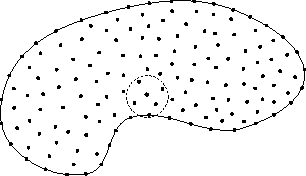
\includegraphics[width=0.7\textwidth]{images/domain_theoretical.pdf}
  \caption[Domena in diskretizacija notranjosti in roba.]{Primer domene z
  diskretnim opisom notranjosti in roba, skupaj z izbrano točko in njeno
soseščino.}
  \label{fig:domain-example}
\end{figure}

V okolici točke $p$ aproksimirajmo $u$ z elementi iz nekega končno
dimenzionalnega prostora funkcij $\B = \Lin\{b_1, \dots, b_m\}$.
Funkcijam $b_i\colon \R^d \to \R$ pravimo \emph{bazne funkcije},
številu $m$ pa moč baze. Ni nujno, da so funkcije $b_i$ definirane
globalno in so lahko odvisne od izbrane točke $p$ in njene soseščine.
Aproksimacijo $\uh$ za $u$ lahko torej zapišemo kot
\begin{equation}
  \label{eq:uhat-def}
   u \approx \uh = \sum_{i=1}^m \alpha_i b_i = \b{b}^\T \b{\alpha},
\end{equation}
pri čemer smo z $\b{\alpha} = (\alpha_i)_{i=1}^m$ označili vektor neznanih
koeficientov in z $\b{b} = (b_i)_{i=1}^m$ funkcijo $\b{b}\colon\R^d\to\R^m$, katere
komponente so bazne funkcije $b_i$.

Če bi poznali vrednosti $u(x_i)$ za $i \in \I(p)$, potem bi za aproksimiranko
$\uh$ v najboljšem primeru zahtevali  $\hat{u}(x_i) = u(x_i)$, za vsak $i \in \I(p)$.
Ker funkcijskih vrednosti $u(x_i)$ ne poznamo, uvedimo spremenljivke $u_i$ za vsako točko v domeni,
ki nam bodo predstavljale neznane prave vrednosti in nadaljujmo s simbolnim računanjem.
Če zahteve za interpolacijo po vrsticah zapišemo v sistem linearnih enačb, dobimo
\begin{equation}
\begin{bmatrix}
  b_1(x_{i_1}) & \cdots & b_m(x_{i_1}) \\
  \vdots & \ddots & \vdots   \\
  b_1(x_{i_n}) & \cdots & b_m(x_{i_n})
\end{bmatrix}
\begin{bmatrix}
  \alpha_1 \\ \vdots \\ \alpha_m
\end{bmatrix}
=
\begin{bmatrix}
  u_{i_1} \\ \vdots \\ u_{i_n}
\end{bmatrix}.
  \label{eq:shape-system}
\end{equation}
Na krajše sistem zapišemo kot $B\b{\alpha} = \b{\tilde{u}}$. Odvisno od $n$, $m$ in $b_i$ je ta
sistem lahko poddoločen, predoločen ali običajen. Vprašanje obrnljivosti matrike $B$ v primeru $n=m$
je težko in je odvisno od izbire funkcij in lege točk. Tudi če so funkcije $b_i$ linearno neodvisne,
obstajajo primeri že v dveh dimenzijah, ko zastavljen interpolacijski problem ni
korekten~\cite[str.\ 79, izrek 2.2]{kozak2008numericna} in zagotavljanje korektnosti v splošnem je
težek problem.

V vsakem primeru lahko definiramo neke vrste rešitev sistema~\eqref{eq:shape-system},
za katero zahtevamo, da minimizira napako v smislu utežene diskretne 2-norme, torej da minimizira
\begin{align}
  \|u-\uh\|_{2, \,\Nc(p), \b{w}} &= \sum_{i\in \I(p)} w(p-x_i) (u_i - \uh(x_i))^2,
\end{align}
pri čemer je $w\colon\R^d\to\R$ nenegativna funkcija, ki jo imenujemo \emph{utež}, $\b{w}$ pa je
vektor sestavljen iz vrednosti te funkcije v točkah v soseščini. Če je takih rešitev $\b \alpha$ več,
izberimo tisto, za katero je $\|\b\alpha\|$ najmanjša. Zgornjo minimizacijo lahko prevedemo na
minimiziranje diskretne 2-norme $\|WB\b{\alpha}-W\b{\tilde{u}}\|_{2, \,\Nc(p)}$, kjer je $W$ diagonalna
matrika korenov uteži za posamezne točke, $W = \diag(\sqrt{w(x_{i_1}-p)}, \dots,
\sqrt{w(x_{i_n}-p)})$. Tak sistem lahko, ne glede na njegovo določenost, rešimo s pomočjo
Moore-Penroseovega psevdoinverza, ki ga izračunamo s pomočjo singularnega razcepa matrike $WB$.
Tako lahko izrazimo \[ \b{\alpha} = (WB)^{+}W\b{\tilde u}, \]
kjer $+$ označuje Moore-Penroseov psevdoinverz.

To lahko vstavimo nazaj v definicijo $\hat{u}$~\eqref{eq:uhat-def} in dobimo
\begin{equation}
  \hat{u} = \b{b}^\T\b{\alpha} = \b{b}^\T(WB)^{+}W\b{\tilde{u}}.
\end{equation}
Sedaj lahko za izbrano točko $p$ izračunamo
\begin{equation}
   \hat{u}(p) = \underbrace{\b{b}(p)^\T(WB)^{+}W}_{\b\phi_p}\b{\tilde{u}}.
\end{equation}
Izračunljivi kos $\b\phi_p$ je v praksi vrstica velikosti $n$, matematično pa je
linearen funkcional $\b\phi_p \in (\R^n)^\ast$, ki naboru funkcijskih vrednosti v
soseščini $\Nc(p)$ priredi aproksimacijo za funkcijsko vrednost v točki $p$.

Podobno kot pri deljenih diferencah odvode funkcije $u$ aproksimiramo z odvodi
interpolacijskega polinoma skozi točke v soseščini, bomo tudi v našem primeru
aproksimirali odvode funkcije $u$ z odvodi $\uh$,
\begin{equation}
  (\L u)(p) \approx (\L \uh)(p) = (\L\b{b})(p)^\T(WB)^{+}W \b{\tilde{u}},
\end{equation}
kjer podobno kot v primeru~\ref{prim:fdm} definiramo
\begin{equation}
  \b\phi_{\L, p} = (\L\b{b})(p)^\T(WB)^{+}W.
  \label{eq:shape-definition}
\end{equation}
Funkcional $\b\phi_{\L, p}$ je aproksimacija operatorja $\L$ v točki $p$. Pogosto se ga imenuje
tudi \emph{funkcija oblike}~\ang{shape function}, saj v sebi nosi podatke o lokalni obliki domene in
izboru okoliških točk ter seveda o obnašanju $\L$ v tej okolici. Tudi če funkcijskih vrednosti
$\b{\tilde{u}}$ v okolici $p$ ne poznamo, lahko $\b\phi_{\L, p}$ izračunamo in kasneje samo s
skalarnim produktom $\b\phi_{\L, p} \b{\tilde{u}}$ dobimo aproksimacijo za $(\L u)(p)$. Lahko pa to
izkoristimo za zapis linearne enačbe
\begin{equation}
  \b\phi_{\L, p} \b{\tilde{u}} = f(p),
\end{equation}
ki je direktna aproksimacija diferencialne
enačbe~\eqref{eq:general-problem} v točki $p$,
\begin{equation}
  \label{eq:discrete-approx-in-one-point}
   (\L u)(p) = f(p).
\end{equation}
Tu ni potrebno, da je $p \in \Nc(p)$, temveč je lahko katerakoli točka v domeni, čeprav bo
najpogosteje tudi sama ena izmed diskretizacijskih točk.

Operatorja $\L$ in $\Rc$ aproksimiramo po celi domeni, tako da za vsako diskretizacijsko točko $x$
v notranjosti izračunamo $\b\phi_{\L, x}$, za vsako točko $y$ na robu pa
$\b\phi_{\Rc, y}$. Za vsako diskretizacijsko točko napišemo
enačbo~\eqref{eq:discrete-approx-in-one-point} in dobimo sistem enačb
\begin{align}
  \b\phi_{\L, x_i} \b{\tilde{u}} &= f(x_i), \text{ za vsak $i$, tak, da je $x_i \in \Omega$ } \\
  \b\phi_{\Rc, x_i} \b{\tilde{u}} &= g(x_i), \text{ za vsak $i$, tak, da je $x_i \in \partial\Omega$.}
\end{align}
Te enačbe lahko zapišemo v matrični sistem
\begin{equation}
  A\b{u} = \b{f},
  \label{eq:discretized-system}
\end{equation}
kjer ima matrika $A$ v vrsticah zapisane funkcije oblike, tako da so neničelni elementi na tistih
mestih, ki se pomnožijo z neznankami, ki ustrezajo sosedom $x_i$. Natančneje, elementi matrike $A$
so
\begin{align}
  A_{k, i_j} &= (\b\phi_{\L, p})_j, \text{ za vsak $k$, tak, da je $x_k \in \Omega$
  in za vsak $i_j \in \I(x_k)$,} \\
  A_{k, i_j} &= (\b\phi_{\Rc, p})_j, \text{ za vsak $k$, tak, da je $x_k \in
  \partial\Omega$ in za vsak $i_j \in \I(x_k)$.}
\end{align}
% Razumljivejša je morda kar Matlab-ova notacija
% \[
% A(k, \I(x_k)) = \begin{cases}
%     \b\phi_{\L, p} & x_k \in \Omega \\
%     \b\phi_{\Rc, p} & x_k \in \partial\Omega \\
%   \end{cases}, \text{ za $k = 1, \ldots, N$}.
% \]
Vektor $\b{u} = (u_i)_{i=1}^N$ je vektor neznanih funkcijskih vrednosti, ki ga
iščemo, v vektorju $\b{f}$ pa so zapisani robni pogoji
\begin{equation}
  \b f_k = \begin{cases}
    f(x_k); & x_k \in \Omega \\
    g(x_k); & x_k \in \partial\Omega \\
  \end{cases}, \text{ za $k = 1, \ldots, N$}.
\end{equation}
Matrika $A$ je razpršena, dimenzij $N\times N$ in v vsaki vrstici ima kvečjemu $n$ neničelnih
elementov, torej je skupno število neničelnih elementov
\begin{equation}
   \nnz(A) \leq nN.
\end{equation}
Enakost je lahko dosežena, lahko pa je tudi stroga, saj so kakšni koeficienti v $\phi_{\L, x_i}$ lahko
tudi 0, kot se to zgodi pri Dirichletovih robnih pogojih.

Rešitev sistema~\eqref{eq:discretized-system} nam da aproksimacijo $u(x_i) \approx u_i$, kar vzamemo
za numerično rešitev problema~\eqref{eq:general-problem}.

\subsection{Posebni primeri}
\label{sec:posebni-primeri}
V metodi iz razdelka~\ref{sec:splosna-izpeljava} lahko v posebnih primerih prepoznamo druge znane
metode. Za začetek pokažimo enostavno trditev, ki bo metodo v določenih primerih poenostavila.
\begin{trditev}
  \label{trd:weight-independence}
  Če je $m = n$ in je matrika $B$ iz sistema~\eqref{eq:shape-system} obrnljiva,
  potem je izbira uteži nepomembna.
\end{trditev}
\begin{proof}
Spomnimo se, da je \[
  \b\phi_{\L, p} = (\L\b{b})(p)^\T(WB)^{+}W.
\]
Matrika $W$ je diagonalna s samimi pozitivnimi števili na diagonali in je torej
obrnljiva. Po predpostavki je obrnljiva tudi matrika $B$, torej je obrnljiv tudi
produkt $WB$ in velja
\[
  (WB)^+ = (WB)^{-1} = B^{-1}W^{-1}.
\]
Od tod sledi, da je
\[
  \b\phi_{\L, p} = (\L\b{b})(p)^\T B^{-1} W^{-1} W = (\L\b{b})(p)^\T B^{-1},
\]
kar je neodvisno od $W$.
\end{proof}
\begin{opomba}
  Čeprav trditev~\ref{trd:weight-independence} velja v eksaktni aritmetiki, v
  praksi ne velja nujno. Če so izbrane uteži zelo majhne ali zelo različnih
  velikosti, lahko to povzroči nepotrebne numerične nestabilnosti. Prav tako
  lahko zaradi izbire uteži pri izračunu psevdoinverza v vrstici~\ref{line:pinv}
  v algoritmu~\ref{alg:shape-function} SVD razcep, uporabljen v ozadju
  funkcije \textsc{pinv}, odreže različno število singularnih vrednosti,
  kar seveda vpliva na rezultate.
\end{opomba}

Če je naš operator enostaven, kot je bil $\dpar{^2}{x^2}$ v primeru~\ref{prim:fdm}
lahko enačbo za funkcije oblike izračunamo direktno. Kaj pa lahko storimo, če je operator bolj
zapleten, ko ne moremo direktno izračunati $\L \b b$? Odgovor na to nudi naslednja trditev.
\begin{trditev}
  \label{trd:shape-linear}
  Preslikava iz vektorskega prostora linearnih parcialnih diferencialnih operatorjev, ki operatorju
  $\L$ priredi funkcijo oblike $\phi_{\L, p} \in (\R^n)^\ast$ v neki točki $p$, je homomorfizem. Za
  $\L = \alpha \L_1 + \beta \L_2$ velja torej
  \begin{equation}
    \b{\phi}_{\alpha \L_1 + \beta \L_2,\,p} =  \alpha \b{\phi}_{\L_1,\,p} + \beta \b{\phi}_{\L_2,\,p}.
  \end{equation}
\end{trditev}
\begin{proof}
Naj bo $\L = \alpha \L_1 + \beta \L_2$. Izračunajmo
  \begin{align*}
    \b{\phi}_{\alpha \L_1 + \beta \L_2,\,p} &=
    ((\alpha \L_1 + \beta \L_2)\b b)(p)(WB)^+W = \\
    &= (\alpha (\L_1\b b)(p) + \beta (\L_2\b b)(p))(WB)^+W = \\
    &= (\alpha (\L_1\b b)(p) + \beta (\L_2\b b)(p))(WB)^+W =\\
  &= \alpha (\L_1\b b)(p)(WB)^+W + \beta (\L_2\b b)(p)(WB)^+W = \\
  &= \alpha \b{\phi}_{\L_1,\,p} + \beta \b{\phi}_{\L_2,\,p}. \qedhere
  \end{align*}
\end{proof}
Zgornja trditev pove, da je za popis vseh linearnih operatorjev do reda $r$ dovolj izračunati le
funkcije oblike za elementarne odvode $D^\omega$ za multiindeks $|\omega| \leq r$. Vsak drug
operator $\L = \sum_{|\omega| \leq r} a_\omega D^\omega$ lahko po linearnosti v vsaki točki
aproksimiramo z elementarnimi aproksimacijami, tako da jih primerno pomnožimo in seštejemo. V tem
primeru ni potrebno, da so $a_\omega$ zgoraj konstante; lahko so tudi funkcije $p$ in v vsaki točki
uporabimo drugače uteženo linearno kombinacijo $D^\omega$. Poseben primer
trditve~\ref{trd:shape-linear}, ki ga bomo pogosto uporabljali, se nanaša na Laplaceov operator,
katerega funkcijo oblike bomo računali kot $\phi_{\lap, p} = \phi_{\dpar{^2}{x^2}, p} +
\phi_{\dpar{^2}{y^2}, p}$.

Že v primeru~\ref{prim:fdm} smo videli, da se za Laplaceov robni problem na
intervalu naša metoda ujema z metodo končnih diferenc. Pokažimo to tudi na
primeru dvodimenzionalne Poissonove enačbe.

\begin{trditev}
  \label{trd:eq-to-fdm}
  Metoda iz razdelka~\ref{sec:splosna-izpeljava} se za reševanje Poissonove
  enačbe na enakomerni pravokotni mreži z razmakom $h$ ujema z metodo končnih
  diferenc pri $\b{b} = \{1, x, y, x^2, y^2\}$, $w \equiv 1$ in
  $n=5$.
\end{trditev}
\begin{proof}
Kot ponavadi označimo točke na mreži s koordinatami $(x_i, y_j)$, tako da je
$x_{i+1} = x_i + h$ in $y_{j+1} = y_j + h$.
Pokazati moramo, da se funkcija oblike v vsaki točki $x$ ujema z aproksimacijo končnih diferenc, ki
pravi
\begin{equation}
  (\lap u)(x_i, y_j) = \frac{u_{i+1,j} + u_{i, j+1} + u_{i-1,j} + u_{i, j-1} - 4u_{i,j}}{h^2},
\end{equation}
pri čemer spremenljivka $u_{i, j}$ pripada koordinati $(x_i, y_j)$. Če se
aproksimaciji Laplaceovega operatorja ujemata, potem se ujemata tudi
aproksimaciji rešitve, saj sistem pri obeh metodah gradimo na enak način.
Ker je operator krajevno neodvisen, so tudi funkcije oblik odvisne samo od
medsebojne lege točk in torej lahko brez škode
za splošnost predpostavimo, da računamo funkcijo oblike za točko
$p = (0, 0)$. Najbližjih $n$ sosedov je tako $\Nc(p) = \{(0, 0), (0, h), (0, -h),
(h, 0), (-h, 0)\}$. Matrika $B$ iz sistema~\eqref{eq:shape-system},
ki ima po stolpcih izračunane bazne funkcije v vseh sosedih je
\begin{equation}
  \label{eq:fdm-special-case-start}
  B =
  \begin{bmatrix}
    1 & 0 & 0 & 0 & 0 \\
    1 & 0 & -h & 0 & h^2 \\
    1 & 0 & h & 0 & h^2 \\
    1 & h & 0 & h^2 & 0 \\
    1 & -h & 0 & h^2 & 0 \\
  \end{bmatrix}
\end{equation}
in njen psevdoinverz, ki je kar njen inverz, je
\begin{equation}
  B^+ = B^{-1} =
  \begin{bmatrix}
     1 & 0 & 0 & 0 & 0 \\
 0 & 0 & 0 & \frac{1}{2 h} & -\frac{1}{2 h} \\
 0 & -\frac{1}{2 h} & \frac{1}{2 h} & 0 & 0 \\
 -\frac{1}{h^2} & 0 & 0 & \frac{1}{2 h^2} & \frac{1}{2 h^2} \\
 -\frac{1}{h^2} & \frac{1}{2 h^2} & \frac{1}{2 h^2} & 0 & 0 \\
  \end{bmatrix}.
\end{equation}
Pri tem smo že upoštevali $w \equiv 1$.
Vektor izračunanih vrednosti operatorja na baznih funkcijah v točki $x$ je
\begin{equation}
   (\lap \b{b})(x) = \begin{bmatrix} 0 & 0 & 0 & 2 & 2 \end{bmatrix}^\T.
\end{equation}
Od tod dobimo po zvezi~\eqref{eq:shape-definition}
\begin{equation}
  \label{eq:fdm-special-case-end}
  \b\phi_\lap = (\lap \b b)(x)^\T B^{+} =
  \begin{bmatrix}
    -\frac{4}{h^2} & \frac{1}{h^2} & \frac{1}{h^2} & \frac{1}{h^2} &
    \frac{1}{h^2}
  \end{bmatrix},
\end{equation}
kar je ravno iskana aproksimacija.
\end{proof}
\begin{opomba}
  Metodo za izračun funkcije oblike je zelo elegantno implementirati v
  Wolfram Mathematici~\cite{mathematica}, kar olajša simbolno raziskovanje takih aproksimacij.
  Enačbe~(\ref{eq:fdm-special-case-start}--\ref{eq:fdm-special-case-end}) so bile izračunane s
  programom~\ref{prog:shape-mathematica}.

\begin{listing}[!h]
    \vspace{-1ex}
  \begin{minted}[frame=lines,linenos,fontsize=\scriptsize]{wolfram}
(* podatki *)
p = {0, 0};
sosedi = {p, {0, -h}, {0, h}, {h, 0}, {-h, 0}};
bazne = {(1 &), (#1 &), (#2 &), (#1^2 &), (#2^2 &)};
operator = Function[f, Function[{x, y}, Derivative[2, 0][f][x, y] + Derivative[0, 2][f][x, y]]];
(* izračun *)
B = Table[Table[b @@ s, {b, bazne}], {s, sosedi}];
Lb = Table[operator[b] @@ p, {b, bazne}];
phi = Lb.PseudoInverse[B] // Simplify
  \end{minted}
  \vspace{-3ex}
  \caption{Računanje funkcij oblike na pravokotni mreži.}
  \label{prog:shape-mathematica}
  \end{listing}
\end{opomba}
\begin{opomba}
  \label{op:fdm-9}
  Tudi če izberemo $n=9$ in $\b b = \{1, x, x^2, y, xy, x^2y, y^2, y^2x, y^2
  x^2 \}$, dobimo enako aproksimacijo kot v trditvi~\ref{trd:eq-to-fdm}, le da
  uporabimo več sosedov. Če jih uredimo po oddaljenosti od $(0, 0)$ dobimo
  aproksimacijo
  \begin{equation}
    \b\phi_\lap =  \begin{bmatrix}
    -\frac{4}{h^2} & \frac{1}{h^2} & \frac{1}{h^2} & \frac{1}{h^2} &
    \frac{1}{h^2} & 0 & 0 & 0 & 0
  \end{bmatrix}.
    \label{eq:shape-mon9}
  \end{equation}
 Če pa bi izbrali $n=25$ točk in bazne funkcije $\b b = \{x^iy^j, 0 \leq i, j
 \leq 4 \}$, bi dobili aproksimacijo četrtega reda.
\end{opomba}
\begin{primer}
  Naredimo še en primer, kjer za bazne funkcije vzamemo monome. Vzemimo tokrat
  $n = 9$ in za bazne funkcije vse monome skupne stopnje manj kot 3, torej $\b b = \{1,
  x, y, x^2, y^2, xy\}$. V tem primeru je matrika $B$ velikosti $9\times 6$ in
  s pomočjo programa~\ref{prog:shape-mathematica} izračunamo
  \begin{equation}
    \b\phi_\lap =
    \begin{bmatrix}
      -\frac{4}{3 h^2} & -\frac{1}{3 h^2} & -\frac{1}{3 h^2} & -\frac{1}{3 h^2} &
      -\frac{1}{3 h^2} & \frac{2}{3 h^2} & \frac{2}{3 h^2} & \frac{2}{3 h^2} &
      \frac{2}{3 h^2}
    \end{bmatrix}.
  \end{equation}
  Vidimo, da tokrat v aproksimaciji upoštevamo vseh 9 sosedov, za razliko od aproksimacije v
  opombi~\ref{op:fdm-9}. Naravno sledi vprašanje, ali je ta aproksimacija drugačnega reda? Izkaže
  se, da ne, saj z razvojem aproksimacij v Taylorjevo vrsto dobimo
  \begin{align}
    &\frac{-4 u(0, 0) + u(0, h) + u(0, -h) + u(h, 0) + u(-h, 0)}{h^2} = \nonumber \\
    & \qquad \qquad = \lap u + \frac{h^2}{12}\left(\dpar{^4u}{x^4}(0, 0) + \dpar{^4u}{y^4}(0, 0)\right) + O(h^4)
  \end{align}
  in
  \begin{align}
    & \frac{-1}{3h^2}(4 u(0, 0) + u(0, h) + u(0, -h) + u(h, 0) + u(-h, 0)) + \phantom{x} \nonumber \\
  & \qquad + \frac{2}{3h^2}(u(h, h) + 2u(h, -h) + 2u(-h, h) + 2u(-h, -h)) = \\
    &\qquad \qquad =
    \lap u + \frac{h^2}{12}\left(\dpar{^4u}{x^4}(0, 0) + \dpar{^4u}{x^2y^2}(0, 0) +
    \dpar{^4u}{y^4}(0, 0)\right) + O(h^4).\nonumber
  \end{align}
  Obe aproksimaciji sta torej drugega reda, razlikujeta se le pri izražavi
  napake.
\end{primer}

\begin{primer}
\label{prim:rbf}
Poglejmo še, kaj se zgodi, če za bazne funkcije vzamemo radialne bazne funkcije in $n = m$, torej
postavimo po eno radialno funkcijo na vsakega izmed sosedov. Opisana metoda tako postane
kolokacijska metoda z lokalnimi radialnimi baznimi funkcijami \ang{local radial basis function
collocation method}~\cite{kosec2011h}.

Če za $n = 9$ sosedov točke $(0, 0)$ izberemo točke
\small
\begin{equation}
  \Nc(p) = \{  (0, 0), (0, h), (0, -h), (h, 0), (-h, 0), (h, h), (h, -h), (-h, h), (-h, -h)\}
\end{equation}
\normalsize
in za $\b b$ vzamemo
\begin{equation}
  \b b = \{ x\mapsto \exp((x-s)^2/\sigma^2); s \in \Nc(p)\},
\end{equation}
potem zopet s pomočjo programa~\ref{prog:shape-mathematica} izračunamo aproksimacijo
\begin{equation}
  \b\phi_\lap =\textstyle \frac{h^2 e^{(h/\sigma)^2}}{\sinh((h/\sigma)^2)^2 \sigma^4}
\begin{bmatrix}
  -\frac{4 + 4(\sigma/h)^2  \sinh((h/\sigma)^2)^2 }{e^{(h/\sigma)^2}} & 1 & 1 & 1 & 1 & 0 & 0 & 0 & 0
 \end{bmatrix}.
  \label{eq:shape-gau9}
\end{equation}
Tokrat vidimo, da se precej razlikuje od aproksimacije s končnimi diferencami.
Toda, še vedno je drugega reda, saj za napako velja
\begin{equation}
  \b \phi_\lap\!\cdot \b{\tilde{u}} - \lap u(0, 0) = \textstyle
  h^2\left(\frac{2u(0, 0)}{\sigma^2} - \frac{\lap u(0, 0)}{\sigma^2} +
  \frac{1}{12}\left( \dpar{^4u}{x^4}(0, 0) + \dpar{^4u}{y^4}(0, 0) \right)\right)
  + O(h^4).
\end{equation}
\end{primer}

Vidimo, da sta aproksimacija operatorja in napaka odvisni od tega, kakšen
$\sigma$ si izberemo v baznih funkcijah.
\begin{trditev}
  \label{trd:rbf-konv-k-mon}
  Aproksimacija Laplaceovega operatorja z devetimi Gaussovimi baznimi funkcijami
  konvergira proti aproksimaciji z monomi, ko gre $\sigma \to \infty$.
\end{trditev}
\begin{proof}
  Obe aproksimaciji smo izračunali že v primeru~\ref{prim:rbf} in
  opombi~\ref{op:fdm-9}. Če pogledamo limito izraza~\eqref{eq:shape-gau9},
  ko gre $\sigma \to \infty$, dobimo izraz~\eqref{eq:shape-mon9}.
\end{proof}

\subsection{Algoritem}
V izpeljavi metode v razdelku~\ref{sec:splosna-izpeljava} je nekaj podrobnosti
ostalo neizdelanih, kot na primer, kako diskretiziramo domeno ali kako poiščemo
sosede. Ti detajli so opisani v naslednjih podrazdelkih, celotna metoda pa je opisana
s pomočjo psevdokode kot algoritem~\ref{alg:metoda}.

\begin{algorithm}[!ht]
  \caption{Brezmrežna metoda za reševanje PDE iz
  razdelka~\ref{sec:splosna-izpeljava}.}
  \textbf{Vhod:} Parcialna diferencialna enačba, opisana
  v~\eqref{eq:general-problem}. Parametri metode: \\
  \begin{tabular}{llll}
    \algorithmlist & $N$     & \ldots & celotno število diskretizacijskih točk    \\
    \algorithmlist & $Q$     & \ldots & število diskretizacijskih točk v
    notranjosti $\Omega$ \\
    \algorithmlist & $n$     & \ldots & število sosedov, ki jih ima vsaka točka   \\
    \algorithmlist & $m$     & \ldots & število baznih funkcij                    \\
    \algorithmlist & $b$ & \ldots & seznam baznih funkcij dolžine $m$         \\
    \algorithmlist & $w$     & \ldots & utež
  \end{tabular} \\
  \textbf{Izhod:} Skalarno polje $u$, ki aproksimira rešitev
  enačbe~\eqref{eq:general-problem}.
  \label{alg:metoda}
  \begin{algorithmic}[1]
    \Function{reši}{$\Omega, \L, f, \Rc, g, N, Q, n, m, b, w$}
    \State $\X \gets \textsc{diskretiziraj}(\Omega, N, Q)$
    \Comment{$\X$ postane seznam $N$ točk, brez škode za splošnost naj leži prvih
    $Q$ točk v $\Omega$ in preostalih $N-Q$ na $\partial \Omega$.}
    \State $s \gets \textsc{sosedi}(\X, n)$ \label{line:kdtree}
    \Comment{$s$ je seznam dolžine $N$, pri čemer je $s[i]$ seznam indeksov
    elementov v $\X$, ki so sosedi $\X[i]$, vključno z $i$.}
    \State $\phi \gets$ prazen seznam dolžine $N$.
    \For{i}{1}{Q} \Comment{Izračunamo funkcije oblik v notranjosti.}
    \State $\phi[i] \gets$ \textsc{funkcijaOblike}$(\L, \X[i], \X, s[i], n, m, b, w)$
    \Comment{Glej algoritem~\ref{alg:shape-function}.}
    \EndFor
    \For{i}{Q+1}{N} \Comment{Izračunamo funkcije oblik na robu.} \label{line:shape-loop}
    \State $\phi[i] \gets$ \textsc{funkcijaOblike}$(\Rc, \X[i], \X, s[i], n, m, b,
    w)$
    \Comment{Glej algoritem~\ref{alg:shape-function}.}
    \EndFor
    \State $A \gets$ prazna razpršena $N\times N$ matrika
    \For{i}{1}{N} \Comment{Aproksimiramo enačbo.}
    \For{j}{1}{n}
    \State $A[i, s[j]] \gets \phi[i][j]$
    \EndFor
    \EndFor
    \State $r \gets$ prazen vektor dolžine $N$
    \For{i}{1}{Q} \Comment{Izračunamo desno stran v notranjosti.}
    \State $r[i] \gets f(\X[i])$
    \EndFor
    \For{i}{Q+1}{N} \Comment{Izračunamo robne pogoje.}
    \State $r[i] \gets g(\X[i])$
    \EndFor
    \State $u \gets$ \textsc{rešiRazpršenSistem}$(A, r)$
    \State \Return $u$
    \EndFunction
  \end{algorithmic}
\end{algorithm}

\begin{algorithm}[!ht]
  \caption{Izračun funkcije oblike.}
  \textbf{Vhod:} Parametri metode: \\
  \begin{tabular}{llll}
    \algorithmlist & $\L$    & \ldots & parcialen diferencialen operator \\
    \algorithmlist & $p$     & \ldots & točka, v kateri aproksimiramo operator \\
    \algorithmlist & $\X$     & \ldots & seznam diskretizacijskih točk \\
    \algorithmlist & $I$     & \ldots & množica indeksov točk v soseščini $p$ \\
    \algorithmlist & $n$     & \ldots & število sosedov, ki jih ima vsaka točka   \\
    \algorithmlist & $m$     & \ldots & število baznih funkcij                    \\
    \algorithmlist & $b$     & \ldots & seznam baznih funkcij dolžine $m$         \\
    \algorithmlist & $w$     & \ldots & utež
  \end{tabular} \\
  \textbf{Izhod:} Funkcional, ki aproksimira operator $\L$ v točki $p$.
  \label{alg:shape-function}
  \begin{algorithmic}[1]
    \Function{funkcijaOblike}{$\L, p, \X, I, n, m, b, w$}
    \State $W \gets$ prazen vektor dolžine $n$
    \For{i}{1}{n}
    \State $W[i] \gets \sqrt{w(\X[I[i]]-p)}$
    \EndFor
    \State $B \gets $ prazna matrika velikosti $n \times m$
    \For{i}{1}{n}
    \For{j}{1}{m}
    \State $B[i, j] \gets W[i] \cdot  b[j](\X[I[i]])$
    \EndFor
    \EndFor
    \State $\ell \gets$ prazen vektor dolžine $m$
    \For{j}{1}{m}
    \State $\ell[j] \gets (\L (b[j]))(p)$
    \EndFor
    \State $\phi \gets (\ell \cdot \textsc{pinv}(B)) \odot W$
    \Comment{Direktna analogija enačbe~\eqref{eq:shape-definition}, $\odot$
  označuje}
    \label{line:pinv}
    \State \Return $\phi$
  \Comment{Hadamardov produkt.}
    \EndFunction
  \end{algorithmic}
\end{algorithm}

\subsubsection{Diskretizacija}
Brezmrežne metode se pogosto oglašuje kot metode, pri katerih je manj težav z diskretizacijo domene
in da lahko kar naključno porazdelimo diskretizacijske točke v domeno. Temu na žalost ni tako, saj
sta natančnost in stabilnost metode odvisni od razporeditve
točk~\cite[slika~8]{kosec2016local},~\cite{amani2012mixed} in je za kvalitetno rešitev potrebno
poskrbeti da so točke čim bolj enakomerno razporejene.

V poljubni $d$-dimenzionalni domeni $\Omega$ je težko dobro razporediti točke.
Uvedimo dve količini, ki merita, kako dobra je diskretizacija domene.
Za dano domeno $\Omega$ in množico diskretizacijskih točk $\X$ definirajmo
\begin{align}
  h_\Omega(\X) &= \max_{p \in \Omega} \min_{x \in \X} \|p - x\| \\
  \label{eq:def-hs}
  S(\X) &= \min_{\substack{x, y \in \X \\ x \neq y}} \|x-y\|.
\end{align}
Količina $h$ pove, kolikšna je maksimalna razdalja do najbližje točke kjerkoli v domeni in intuitivno
opisuje, kako dobro smo z diskretizacijskimi točkami pokrili domeno. Največji krog, ki ga lahko
narišemo v domeni, ne da bi v notranjosti vseboval kakšno diskretizacijsko točko, je ravno radija
$h_\Omega(\X)$. Količina $S$ pove, kolikšna je najmanjša razdalja med dvema sosednjima točkama in
karakterizira stabilnost metode. Dobra diskretizacija želi pri danem številu točk maksimizirati $S$
in minimizirati~$h$.

Pri domenah lepih oblik kot so kvadri in krogle, lahko uporabimo znane algoritme za regularne
diskretizacije. Tako lahko za diskretizacijo kvadra uporabimo kar enakomerno diskretizacijo. Za
čimbolj enakomerno diskretizacijo notranjosti kroga ali površine sfere lahko uporabimo
npr.~Fibonaccijevo mrežo, kot predlagano v~\cite{hannay2004fibonacci}
ali~v~\cite{gonzalez2010measurement}.
Z nekaj osnovnimi operacijami kot so unija in razlika množic lahko opišemo že dokaj zanimive oblike
(slika~\ref{fig:domains}).

\begin{figure}[!ht]
  \centering
  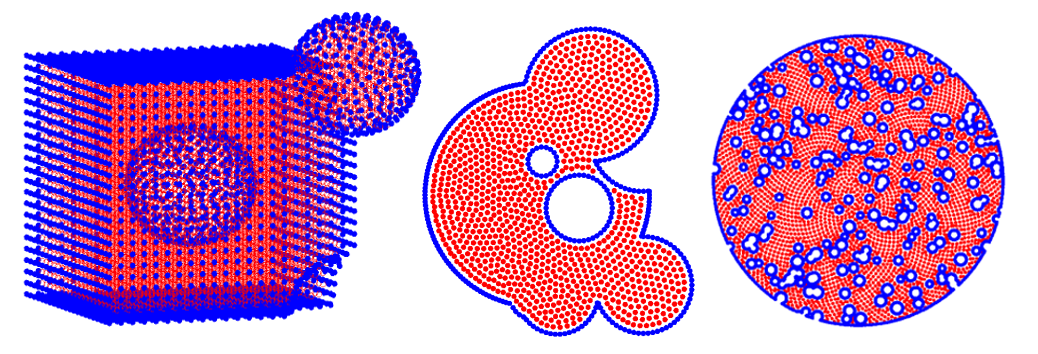
\includegraphics[width=\textwidth]{images/domains_generated.png}
  \caption{Primeri bolj zapletenih domen in njihovih diskretizacij.}
  \label{fig:domains}
\end{figure}

Pogosto pa nimamo opravka z domenami pravilnih oblik in želimo splošnejši algoritem, ki potrebuje
samo implementacijo operacije $p \in \Omega$. Ker je domena omejena, je vsebovana v nekem
$d$-dimenzionalnem kvadru in lahko diskretizacijo $\Omega$ konstruiramo tako, da vzamemo enakomerno
diskretizacijo tega kvadra ter odstranimo vse točke, ki niso v domeni. Druga metoda je, da
naključno izbiramo točke v kvadru, in sprejmemo tiste, ki pristanejo v notranjosti $\Omega$. Še
boljšo diskretizacijo dobimo, če namesto psevdonaključnih števil pri izbiranju točk
uporabimo kvazinaključna števila, ki imajo manjšo diskrepanco~\cite{morokoff1994quasi} in so zato
bolj primerna. Kljub njihovi splošnosti so naključne diskretizacije precej slabe, kot lahko vidimo
na enakomerni naključni diskretizaciji kroga na sliki~\ref{fig:relax-circle} (levo).

Vendar ni še vse izgubljeno, saj lahko zgoraj opisane enostavne postopke za diskretizacijo
uporabimo, da dobimo začetni približek za boljšo diskretizacijo. Pri tem, da bi ta približek
izboljšali in točke v domeni porazdelili čimbolj enakomerno, si lahko pomagamo s preprostim
iterativnim postopkom, za katerega se izkaže, da v praksi dobro deluje. Navdih jemljemo iz fizike in
si zamislimo, da je vsaka točka naboj, ki se odbija od sosednjih točk. Na vsako točko tako deluje
sila, porojena z nekim potencialom, ki jo sili stran od drugih točk, v prazen prostor. Točko lahko
malo premaknemo v smeri sile, ponovno izračunamo medsebojne sile in postopek ponavljamo. Pri tem
točkam na robu ne dovolimo premikanja in če kakšna točka iz notranjosti zleze iz domene, jo
postavimo nazaj na naključno mesto v domeno. Zapis zgornjega postopka je v psevdokodi podan kot
algoritem~\ref{alg:relax}. Postopek se imenuje \emph{sprostitev} \ang{relaxation}
domene~\cite[razdelek~2.2]{kosec2016local}, kajti na začetku so med točkami napetosti, ki jih s
premikanjem minimiziramo. Rezultati opisanega postopka na primeru izboljšanja naključne
diskretizacije kroga so prikazani na sliki~\ref{fig:relax-circle} (desno).

\begin{algorithm}[!ht]
  \caption{Algoritem za izboljšanje kvalitete diskretizacije domene.}
  \textbf{Vhod:} Parametri metode: \\
  \begin{tabular}{llll}
    \algorithmlist & $\Omega$  & \ldots & domena \\
    \algorithmlist & $N$       & \ldots & število diskretizacijskih točk \\
    \algorithmlist & $Q$       & \ldots & število diskretizacijskih točk v
    notranjosti $\Omega$ \\
    \algorithmlist & $\X$       & \ldots & seznam diskretizacijskih točk, prvih $Q$
    je v notranjosti. \\
    \algorithmlist & $I$       & \ldots & število iteracij \\
    \algorithmlist & $s$       & \ldots & število sosedov, ki jih upoštevamo pri delovanju sile \\
    \algorithmlist & $F_0$     & \ldots & delež sile, ki vpliva na premik \\
    \algorithmlist & $\alpha$  & \ldots & eksponent v sili                \\
  \end{tabular} \\
  \textbf{Izhod:} Nov seznam diskretizacijskih točk.
  \label{alg:relax}
  \begin{algorithmic}[1]
    \Function{izboljšaj}{$\Omega, N, Q, \X, I, s, F_0, \alpha$}
    \State $r_\chi \gets \left( \frac{\textsc{volumen}(\Omega)}{N}
    \right)^{\frac{1}{\textsc{dimenzija}(\Omega)}}$ \Comment{Približek povprečne
    razdalje med točkami}. \label{line:chd}
    \For{i}{1}{I}
    \For{j}{1}{Q}
    \State $\vec{F} \gets \vec{0}$
    \ForEach{y}{\{najbližjih $s$ sosedov $\X[i]$\}} \label{line:closest}
    \State $\vec{r} \gets \frac{\X[i] - y}{r_\chi}$ \Comment{Brezdimenzijski vektor
    razdalje.}
    \State $\vec{F} \gets \vec{F} + \frac{\vec{r}}{\|\vec{r}\|^\alpha}$
    \EndFor
    \State $\X[i] \gets \X[i] + F_0 \vec{F}$.
    \If{$\X[i] \notin \Omega$}
    \State $\X[i] \gets $ naključna pozicija znotraj $\Omega$
    \EndIf
    \EndFor
    \EndFor
    \State \Return $\X$
    \EndFunction
  \end{algorithmic}
\end{algorithm}

\begin{figure}[!ht]
  \centering
  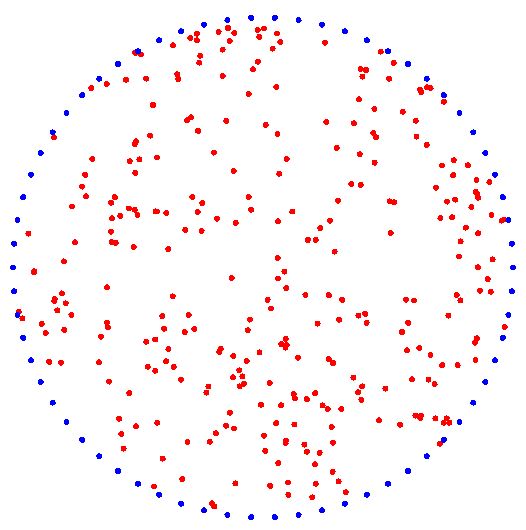
\includegraphics[width=0.3\textwidth]{images/domain_circle.png}
  \hspace{1em}
  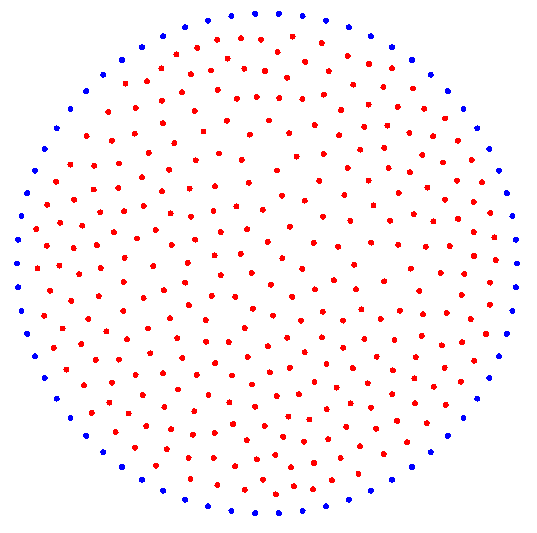
\includegraphics[width=0.3\textwidth]{images/domain_circle_relaxed.png}
  \caption[Primerjava naključno diskretizirane in izboljšane domene.]{Primerjava domene z naključno
  diskretizacijo (levo) in domene po izvedbi 10 iteracij algoritma~\ref{alg:relax} s parametri $F_0
  = 10^{-2}$, $s = 6$, $\alpha = 3$ (desno).}
  \label{fig:relax-circle}
\end{figure}

Da algoritem izboljša kvaliteto aproksimacije se vidi tudi, če izračunamo
parametra $h$ in $S$. Na sliki~\ref{fig:relax-hs} vidimo primerjavo med
kvaliteto diskretizacije s Fibonaccijevo mrežo in njeno 30-kratno izboljšavo.
Vidimo, da se je $h$ nekoliko izboljšal, za ceno večje variance,
$S$ pa se je precej izboljšal in izkazuje celo lepše obnašanje kot prej.

\begin{figure}[ht]
  \centering
  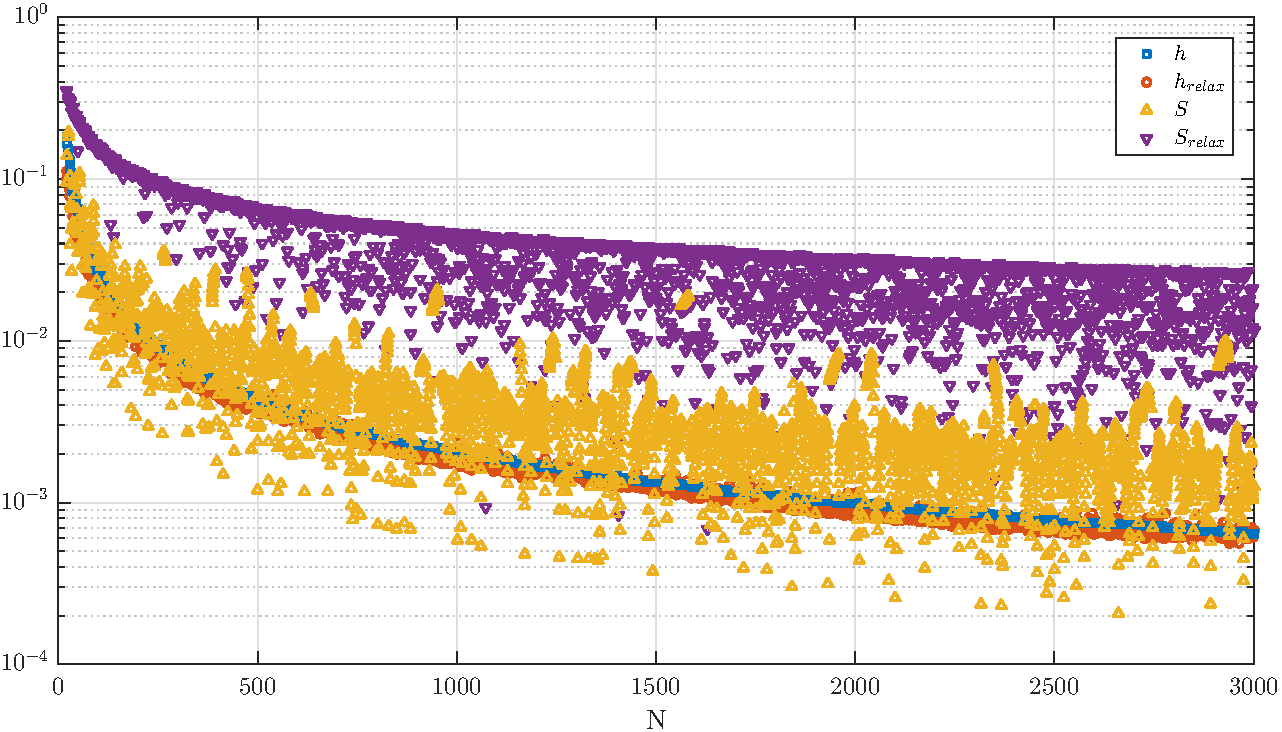
\includegraphics[width=\iw]{images/relax_improvement.pdf}
  \caption[Sprememba kvalitete diskretizacije po izboljšavi.]{Sprememba $h$ in
    $S$ po 30 iteracijah algoritma~\ref{alg:relax} s parametri $F_0 = 10^{-2}$,
    $s = 6$, $\alpha = 3$ v enotskem dvodimenzionalnem krogu z začetno
    Fibonaccijevo mrežo, v odvisnosti od $N$, z razmerjem robnih in notranjih
  točk $x : \frac{12}{\pi} \sqrt{x}$.}
  \label{fig:relax-hs}
\end{figure}

\subsubsection{Goščenje diskretizacije}
\label{sec:goscenje}
Pri reševanju problemov z divje spreminjajočimi rešitvami, singularnostmi ali zelo majhnimi
lokalnimi fenomeni si pogosto pomagamo z lokalnim zgoščevanjem krajevne diskretizacije v okolici
dela rešitve, ki nas najbolj zanima. Pri metodah, ki temeljijo na triangulaciji domene, lahko
trikotnike v območju interesa delimo in tako dobimo finejšo triangulacijo. Pri brezmrežnih
metodah želimo doseči enak učinek, zato potrebujemo način, da gostimo točke na nekem območju.
Postopek bomo imenovali \emph{goščenje} \ang{refinement}.

Izberimo točko $p$ okoli katere bomo gostili diskretizacijo. Pri opisu postopka si pomagajmo z
ilustracijo na sliki~\ref{fig:refine-algorithm}.
\begin{figure}[h]
  \centering
  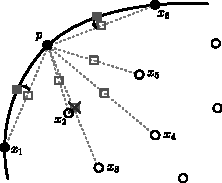
\includegraphics[width=0.5\textwidth]{images/domain_refine.pdf}
  \caption{Algoritem za goščenje točk v domeni.}
  \label{fig:refine-algorithm}
\end{figure}
Poiščimo najbližjih $\ell$ sosedov točke $p$, pri čemer ne štejemo $p$ in jih označimo z $L = \{x_1,
\dots, x_\ell\}$. Za vsakega izmed sosedov dodamo novo točko, na polovici daljice med $x_i$ in $p$,
označeno s sivim kvadratkom. Kandidati za nove diskretizacijske točke so torej
\begin{equation}
   \X' = \left\{ \frac{p+x}{2}; x \in L \right\}.
\end{equation}
Pri tem pazimo, da če sta tako $x$ kot $p$ točki na robu, je tudi njuno središče robna točka in jo
projiciramo na rob domene, kot prikazano na primeru na sliki~\ref{fig:refine-algorithm} z dvema
potemnjenima kvadratkoma. Če je katera izmed točk v $\X'$ izven $\zomega$, jo odstranimo iz množice
kandidatov. Poleg tega se lahko zgodi, da so nekatere nove točke preblizu skupaj ali pa preblizu
starim točkam, kar bi povzročilo nestabilnosti pri računanju funkcij oblike. Zato v parih točk, ki
so bolj skupaj kot dovoljena razdalja $r_{\text{min}}$ zavržemo novejšo točko, če je ta preblizu
kakšni stari. Za razdaljo $r_\text{min}$ ponavadi vzamemo $r_\text{min} = f r_c$, kjer je $r_c$
razdalja do najbližjega soseda~\eqref{eq:min-dist} in $f$ pozitiven faktor, ponavadi manjši od
$\nicefrac{1}{2}$.

Zgornji postopek je lokalne narave in njegovo izvajanje je, zaradi iskanja sosedov, le logaritemsko
odvisno od števila točk v domeni. Če želimo na nekem območju še gostejšo diskretizacijo, postopek
preprosto ponovimo večkrat zapored. Primer večkrat zgoščene domene je prikazan na
sliki~\ref{fig:hertz-refined-domain-together} na strani~\pageref{fig:hertz-refined-domain-together}.

\subsubsection{Iskanje najbližjih sosedov}

Tako v algoritmu~\ref{alg:metoda} na vrstici~\ref{line:kdtree}, kot v algoritmu~\ref{alg:relax} na
vrstici~\ref{line:closest} je potrebno poiskati najti nekaj najbližjih sosedov dane točke. Problem
iskanja najbližjih sosedov \ang{nearest neighbour search} je znana in dobro raziskana tema z
razvitimi veliko podatkovnimi strukturami, ki podpirajo grajenje, iskanje, vstavljanje in brisanje v
logaritemskem času. Večina jih temelji na delitvi prostora na različne hierarhično urejene
podprostore, ki jih potem hranimo v drevesni strukturi, kar nam omogoča logaritemski dostop. Med
bolj znanimi strukturami so \emph{$k$-d tree}~\cite{moore1991intoductory}, \emph{ball
tree}~\cite{omohundro1989five} in \emph{cover tree}~\cite{beygelzimer2006cover}. V
članku~\cite{kibriya2007empirical} je narejena empirična primerjava med zgornjimi tremi strukturami,
ki pokaže, da se v primeru nizkih dimenzij (kar gotovo vsebuje $d \leq 3$) najbolje obnese
$k$-d drevo. Poleg tega $k$-d drevo najbolje deluje tudi, ko imajo točke, v katerih
bomo iskali sosede, podobno porazdelitev kot točke, iz katerih smo naredili drevo, kar v našem
primeru drži. Če vključimo še dejstvo, da je $k$-d drevo tudi najpopularnejša rešitev za
problem najbližjih sosedov in ima na voljo veliko prosto dostopnih implementacij, je to dovolj
argumentov, da jo uporabimo tudi mi. Specifična uporabljena implementacija je predstavljena
v~\cite{mount1998ann}, ki za shrambo $N$ točk porabi $O(N)$ prostora in odgovarja na poizvedbe o $n$
najbližjih sosedih v $O(n\log N)$ časa. S pomočjo tega postane implementacija funkcije
\textsc{sosedi} iz algoritma~\ref{alg:metoda} trivialna, pri algoritmu~\ref{alg:relax} pa si na
vsaki iteraciji na novo zgradimo drevo in ga uporabimo za iskanje $s$ najbližjih sosedov.

\subsubsection{Reševanje razpršenega sistema}
\label{sec:solve-sparse}
Za reševanje razpršenih sistemov poznamo veliko različnih metod, ki se v grobem delijo na
direktne~\cite{davis2006direct} in iterativne~\cite{saad2003iterative}. Pri običajnih, polnih
matrikah bi za reševanje splošnega sistema linearnih enačb uporabili LU razcep in razcepili matriko
$A$ kot $A = LU$. Toda, tudi če je matrika $A$ razpršena, v splošnem $L$ in $U$ nista nujno in sta
lahko celo polni, kar povzroči, da nam zmanjka pomnilnika. Direktne metode, kot na primer
SuperLU~\cite{li2005overview} poskušajo s preureditvijo stolpcev v razpršeni matriki $A$
minimizirati število novih neničelnih elementov v matrikah $L$ in $U$. Po drugi strani iterativne
metode aproksimirajo pravilno rešitev sistema $Ax=b$ z zaporedjem približkov $\{x^{(r)}\}$, ki naj
bi konvergirali k $x$. Te metode običajno ne zahtevajo veliko pomnilnika, je pa natančnost približka
odvisna od števila porabljenih iteracij, ali drugače, z višanjem želene natančnosti raste tudi
računska zahtevnost.

V primerih, predstavljenih v tem delu, uporabljamo knjižnico Eigen~\cite{eigenweb}, ki nudi
elegantno in hitro delo z matrikami v \CC. Vgrajenih ima več direktnih in iterativnih metod za
reševanje sistemov linearnih
enačb.\footnote{\url{https://eigen.tuxfamily.org/dox/group__TopicSparseSystems.html}
[ogled 17.\ 6.\ 2017]}
Pri sistemih tipa~\eqref{eq:discretized-system} se je v praksi najbolje obnesel
BiCGSTAB~\cite{van1992bi} z ILUT predpogojevanjem~\cite{saad1994ilut}. BiCGSTAB v primeru uporabe
pravilne shrambe matrike v pomnilniku podpira tudi paralelizacijo, poleg tega pa je konvergenca v
praksi dovolj hitra. Predpogojevanje z uporabo nepopolnega LU razcepa z dvojnim pragom~\ang{dual
threshold incomplete LU factorization (ILUT)} omogoča natančnejšo kontrolo nad porabljenim spominom
in hitrostjo konvergence z uporabo dveh parametrov $p$ in $\tau$. Med $LU$ faktorizacijo izpustimo
vsak element, ki je manjši kot $\tau\cdot e$, kjer je $e$ povprečna absolutna vrednost elementov v
trenutni vrstici. Nato obdržimo le največjih $f$ elementov v matrikah $L$ in $U$, kjer je $p$
uporabljen kot razmerje med $f$ in začetnim številom neničelnih elementov. V grobem tako parameter
$p$ kontrolira kolikokrat več spomina dovolimo za hranjenje predpogojenke, parameter $\tau$ pa kako
natančna bo LU faktorizacija.

\subsubsection{Časovna zahtevnost}
\label{sec:casovna-zahtevnost}
Pri analizi časovne zahtevnosti metode bomo predpostavili, da so
vse evalvacije funkcij $f$, $g$, $w$ in $b_j$, $\L b_j$, $\Rc b_j$ izvedene v $O(1)$.
Prav tako bomo predpostavili, da je dimenzija problema majhna in konstantna in
ne bo nastopala v analizah.

\begin{trditev}
  Pričakovana časovna zahtevnost algoritma~\ref{alg:metoda} je
  \begin{equation}
    O(I N s \log^2 N + (N+n)\log N + m^2n N) + T,
    \label{eq:casovna-zahtevnost}
  \end{equation}
  kjer je $T$ čas, porabljen za reševanje razpršenega sistema enačb.
\end{trditev}
\begin{proof}
Pri funkciji \textsc{diskretiziraj} predpostavimo, da uporabljamo enostavno
diskretizacijo, ki deluje v $O(N)$ časa, skupaj z $I$ iteracijami izboljšave
na $s$ sosedih, ki traja $O(I N s \log^2 N)$ časa, saj na vsaki iteraciji
konstruiramo drevo in iščemo $s$ sosedov vsake točke.

Izvajanje funkcije \textsc{sosedi} potrebuje $O((N+n) \log N)$ časa za konstrukcijo
drevesa in iskanje sosedov.

Izvajanje funkcije \textsc{funkcijaOblike} traja $O(n + nm + m + m^2n + nm +
n) = O(m^2n)$ časa, kjer je prevladujoči faktor $O(m^2 n)$ rezultat računanja SVD
razcepa z dvostranskim Jacobijevim SVD razcepom iz knjižnice
Eigen.\footnote{\url{https://eigen.tuxfamily.org/dox/classEigen_1_1JacobiSVD.html}
[ogled 16.\ 6.\ 2017]} Funkcija oblike se izračuna za vsako točko v domeni,
kar doprinese $O(m^2 n N)$ k skupni zahtevnosti.

Pri sestavljanju razpršene matrike lahko v naprej rezerviramo prostor za $n$
elementov v vsaki vrstici, tako da sestavljanje matrike stane $O(nN)$ časa,
sestavljanje robnih pogojev pa $O(N)$ časa. Na koncu še rešimo razpršen sistem
linearnih enačb, kjer pa je čas zelo odvisen od problema, iteracijske metode in
predpogojenke.

Skupna časovna zahtevnost je tako $O(I N s \log^2 N + (N+n)\log N + m^2n N) + T$,
kjer je $T$ čas, porabljen za reševanje razpršenega sistema enačb.
\end{proof}

\subsubsection{Prostorska zahtevnost}
Podobno kot pri časovni zahtevnosti bomo predpostavili, da so vse evalvacije funkcij $f$, $g$, $w$
in $b_j$, $\L b_j$, $\Rc b_j$ izvedene v $O(1)$ prostora. Prav tako bomo predpostavili, da je
dimenzija problema majhna in konstantna in ne bo nastopala v analizah.

\begin{trditev}
  Prostorska zahtevnost algoritma~\ref{alg:metoda} je $O(nN) + P$, kjer je $P$
  prostor, potreben za reševanje sistema linearnih enačb.
\end{trditev}
\begin{proof}
Pri funkciji \textsc{diskretiziraj} potrebujemo $O(N)$ spomina za hrambo $N$
diskretizacijskih točk. Če izvajamo še dodatne izboljšave diskretizacije, nas to
stane $O(n)$ dodatnega prostora.

Za izvajanje funkcije \textsc{sosedi} porabimo $O(N)$ prostora za hranjenje drevesa
in $O(nN)$ prostora za hranjenje indeksov $n$ sosedov.

Izvajanje funkcije \textsc{funkcijaOblike} nas stane $O(n+nm+m+n) = O(nm)$
prostora za vsak klic, za hrambo $N$ funkcij oblike pa potrebujemo $O(nN)$
prostora.

Razpršena matrika prav tako potrebuje $O(nN)$ prostora za neničelne elemente.
Nato moramo rešiti le še sistem linearnih enačb, kar po predpostavki stane $P$
prostora. Ker je $m = O(N)$ je prevladujoči faktor $O(nN)$ in skupna prostorska
zahtevnost je $O(nN) + P$.
\end{proof}

\subsection{Pogoste vrednosti parametrov}
Metoda je bila do sedaj formulirana zelo splošno, v praksi pa se uporablja nekaj
ustaljenih kombinacij. Kot bomo videli, razdalje pogosto merimo v večkratnikih
$r_\chi$, kot v vrstici~\ref{line:chd} v algoritmu~\ref{alg:relax}.
\begin{definicija}
  Količino $r_\chi$, pripisano diskretizaciji $\X$ domene $\Omega$, izračunano z
  \begin{equation}
    r_\chi(\Omega, \X) = \left( \frac{\textsc{volumen}(\Omega)}{|\X|}
    \right)^\frac{1}{\textsc{dimenzija}(\Omega)},
  \end{equation}
  imenujemo \emph{karakteristična razdalja.}
\end{definicija}
Ideja definicije je, da $r_\chi$ predstavlja približno povprečno razdaljo med
diskretizacijskimi točkami, če bi bile razporejene enakomerno. Celoten volumen
domene razdelimo na $N = |\X|$ delov, tako da vsaki točki pripada enak kos
volumna $v = \frac{\textsc{volumen}(\Omega)}{N}$. Če bi
bil ta kos neka hiperkocka v $d$ dimenzijah, potem je $\sqrt[d]{v}$ dolžina
njene stranice in to je ocena za medsebojno razdaljo med točkami.
V eni dimenziji $r_\chi$ do faktorja $\frac{N}{N-1}$ natančno ustreza razdalji
med enakomerno razporejenimi točkami.
Drugo pogosto merilo za lokalno razdaljo bo kar razdalja do najbližjega
(različnega) soseda, ki jo imenujmo $r_c$,
\begin{equation}
  r_c(p) = \min_{\substack{x \in \Nc(p) \\ x \neq p}} \|x-p\|.
  \label{eq:min-dist}
\end{equation}
To je težje izračunati, če nimamo že
zgrajenega drevesa, zato se ponavadi na enostavnejših primerih poslužujemo kar
$r_\chi$. Kadar pa to ni dobra aproksimacija razdalje med vozlišči za celo
domeno, kot na primer ob goščenju mreže, se poslužimo $r_c$.

Pogoste vrednosti za število sosedov so $n = 3, 5, 7$ v eni dimenziji, $n = 5, 9, 13, 25$ v dveh
dimenzijah in $n = 7$ ali $27$ v treh dimenzijah. Za regularno porazdeljene točke v domeni to
pomeni, da so vozlišča izbrana simetrično, pri neregularnih pa izbira $n$ ni tako pomembna, dokler
je dovolj visoka, da dobro popiše operator, ki ga aproksimiramo. Višji $n$ ponavadi pomeni večjo
stabilnost, morda višji red in počasnejše izvajanje. V praksi izberemo najmanjši $n$, ki zagotovi
zadovoljive rezultate.

Za utež se pogosto uporablja konstanta $w\equiv1$, če ne želimo uteženih
najmanjših kvadratov, sicer pa pogosto vzamemo za utež Gaussovo funkcijo
\begin{equation}
   w(x) = \exp\left(-\left(\frac{x}{\sigma_w}\right)^2 \right),
\end{equation}
kjer $\sigma_w$ imenujemo parameter oblike \ang{shape parameter} uteži.
Velja opozoriti, da je ta funkcija praktično nič, če smo več kot $3\sigma_w$
stran od središča ($w(3\sigma_w) \approx 0.0001234$). Če na primer izberemo
$\sigma_w = r_\chi$ se vsi sosedi, ki so dlje kot $r_\chi$ stran, v
aproksimaciji ne upoštevajo, ne glede na to kako velik $n$ smo izbrali.
Ponavadi se za $\sigma_w$ začne izbirati vrednosti okoli $r_\chi$, je
pa potrebno optimalno vrednost določiti za vsak posamezen problem posebej.

Pogosta izbira baznih funkcij so prostori $\mathbb{P}_\ell$ monomov skupne
stopnje manj ali enako $\ell$. Pri tem moramo seveda paziti, da izberemo dovolj
visok $n$. Druga pogosta izbira je, da vzamemo $m = n$ in za bazne funkcije
izberemo radialne bazne funkcije s centri v sosedih~\cite{kosec2011h}.

\begin{definicija}
  Funkcija $\psi_c$ se imenuje radialna bazna funkcija s centrom v točki $c$, če je odvisna samo od
  razdalje do centra, torej
  \begin{equation}
    \psi_c(x) = \tilde\psi(\|x - c\|),
  \end{equation}
  za vsak $x$ za neko funkcijo $\psi$. Kasneje kar identificiramo $\psi_c$
  in $\tilde\psi$ in pišemo $\psi_c = \psi_c(r)$.
\end{definicija}

\begin{figure}[h]
  \centering
  \begin{subfigure}[t]{0.33\textwidth}
    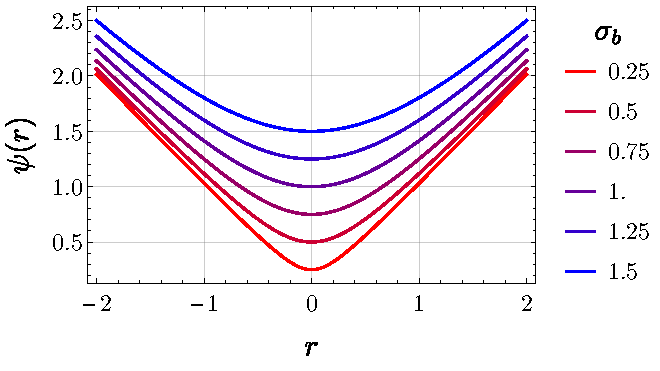
\includegraphics[width=\textwidth]{images/rbf_mq.pdf}
    \caption[Multikvadratične]{Multikvadratične \\ \ang{Multiquadric}  \\ $\psi(r) = \sqrt{r^2+\sigma_b^2}$}
  \end{subfigure}
  \begin{subfigure}[t]{0.33\textwidth}
    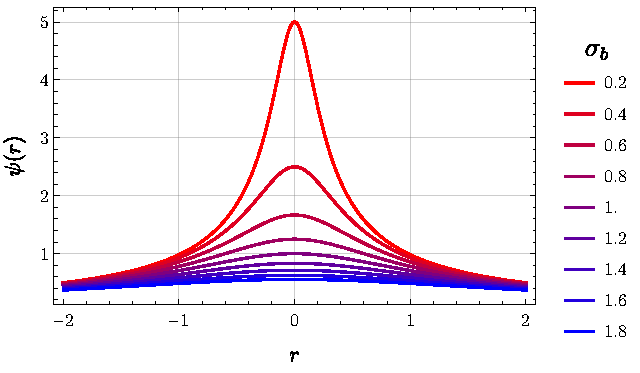
\includegraphics[width=\textwidth]{images/rbf_imq.pdf}
    \caption[Inverzne multikvadratične]{Inverzne multikvadratične \\ \ang{Inverse multiquadrics}  \\ $\psi(r) = 1 / \sqrt{r^2+\sigma_b^2}$}
  \end{subfigure}
  \begin{subfigure}[t]{0.32\textwidth}
    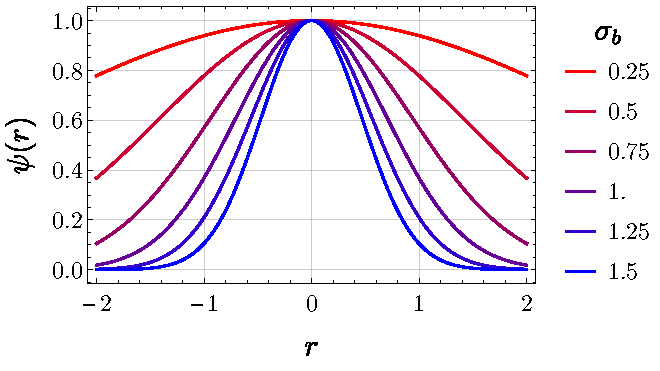
\includegraphics[width=\textwidth]{images/rbf_gau.pdf}
    \caption[Gaussove funkcije]{Gaussove funkcije \\ \ang{Gaussians} \\ $\psi(r) = \exp(-(r/\sigma_b)^2)$}
  \end{subfigure}
  \caption[Najpogosteje uporabljene radialne bazne funkcije]{Najpogosteje uporabljene radialne bazne
  funkcije s parametrom oblike $\sigma_b$.}
  \label{fig:rbf}
\end{figure}

% \newcommand{\tc}[1]{\vspace{-15ex}\parbox{6cm}{#1}}
% \begin{table}[!h]
%   \centering
%   \begin{tabular}{|m{6.2cm}|l|} \hline
%     \tc{} & 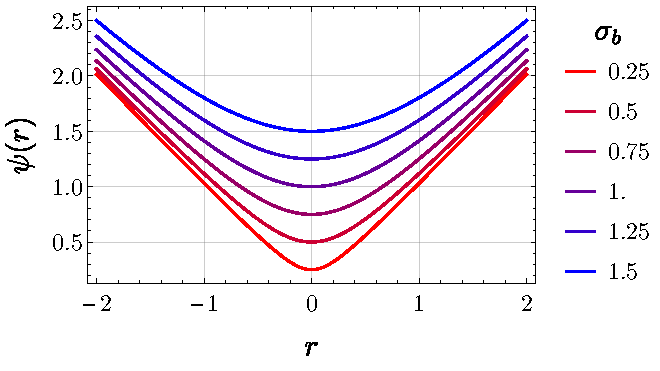
\includegraphics[width=0.33\textwidth]{images/rbf_mq.pdf} \vspace{-1ex} \\ \hline
%     \tc{} & 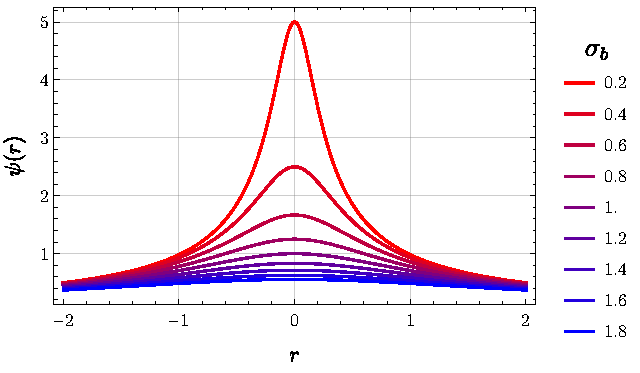
\includegraphics[width=0.33\textwidth]{images/rbf_imq.pdf} \vspace{-1ex} \\ \hline
%     \tc{} &
%     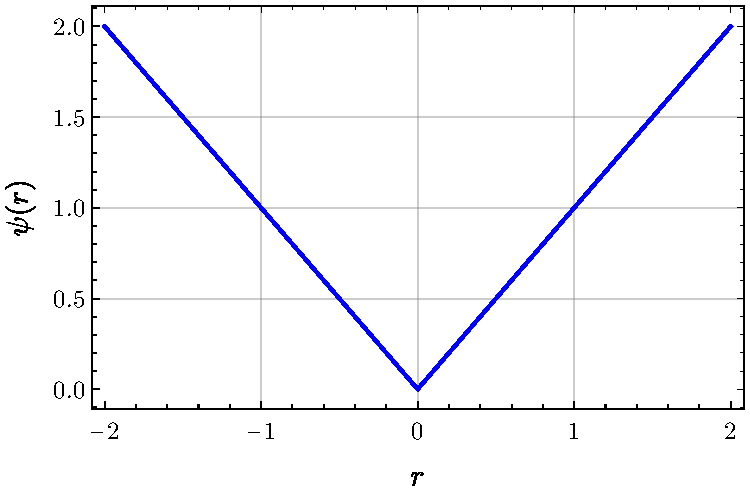
\includegraphics[width=0.278\textwidth]{images/rbf_lin.pdf} \vspace{-1ex} \\ \hline
%     \tc{} & 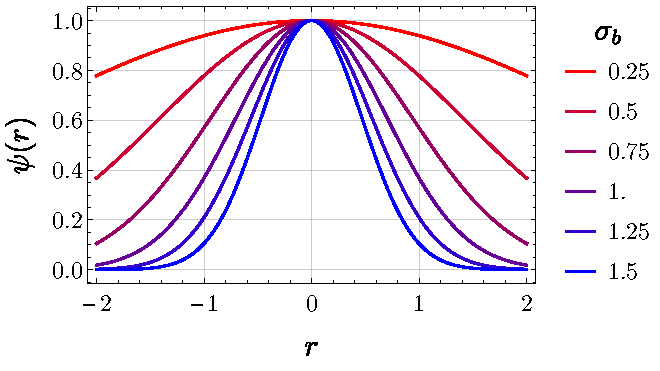
\includegraphics[width=0.33\textwidth]{images/rbf_gau.pdf} \\ \hline
%   \end{tabular}
% \end{table}


Na sliki~\ref{fig:rbf} so naštete najpogostejše uporabljene radialne bazne funkcije, povzete
po~\cite[str.\ 5]{schaback1995error}.
Ko si izberemo neko bazno funkcijo $\psi$, potem za bazne funkcije okoli točke
$p$ vzamemo
\begin{equation}
   \b b = \{\psi_s; s \in \Nc(p) \}.
\end{equation}
Pri izbiri parametra oblike $\sigma_b$ moramo tudi biti do neke mere pazljivi. Izbrati
ga moramo dovolj velikega, da se funkcije ``prekrivajo'', torej tako, da nima
funkcija vrednosti blizu nič pri vseh sosedih razen pri sebi. Hkrati mora biti
parameter dovolj majhen, da sistem~\eqref{eq:shape-system} ni preveč nestabilen.
Bolj natančna analiza izbire parametra oblike za radialne bazne funkcije in
za utež je narejena na sliki~\ref{fig:poisson-square-sigma-dep} med numeričnimi
zgledi na strani~\pageref{fig:poisson-square-sigma-dep}.

Pogosto se k bazi radialnih baznih funkcij doda še monome nizkih stopenj, za
boljšo aproksimacijo funkcij, ki so blizu konstantam. Več o kvaliteti,
stabilnosti in redu konvergence aproksimacije z radialnimi baznimi funkcijami
si lahko bralec prebere v~\cite{buhmann2000radial}.

\section{Osnovni numerični zgledi}
\label{sec:osnovni-zgledi}
V tem razdelku si bomo ogledali obnašanje metode na čedalje bolj zapletenih numeričnih zgledih, da
si zgradimo intuicijo o njenem delovanju in da se pripravimo na reševanje problema iz mehanike
utrujenosti materialov, opisanega v uvodu. V nadaljnjem besedilu in na vseh grafih bo metoda,
opisana v razdelku~\ref{sec:numericna-metoda} označena s kratico MLSM \ang{Meshless Local Strong
Form Method}. Če ni drugače navedeno, so vse meritve narejene na računalniku z eno centralno
procesno enoto \verb|Intel(R) Core(TM) i7-4700MQ CPU @2.40GHz| s štirimi jedri, od katerih vsako
podpira dve niti izvajanja, in \unit[16]{GiB} DDR3 pomnilnika. Vsi programi so bili prevedeni s
prevajalnikom \verb|g++| verzije 7.1.7 in stikali \verb|-std=c++14 -O3 -DNDEBUG| na operacijskem
sistemu Manjaro Linux.

\subsection{Enodimenzionalni robni problem}
Oglejmo si najprej preprost primer reševanja enodimenzionalne Poissonove enačbe, ki smo ga uporabili
že za motivacijo izpeljave numerične metode. Rešujmo problem
\begin{align}
  u''(x) &= \sin(x), \quad x \in (0, 1) \nonumber \\
  u(0) &= 0,  \\
  u'(1) &= 0, \nonumber
\end{align}
ki ima analitično rešitev $u(x) = \cos(1) x - \sin(x)$.
Na sliki~\ref{fig:mlsm-fdm-err} je prikazana konvergenca metode končnih diferenc
in MLSM. Metoda MLSM je bila uporabljena s parametri, pri katerih velja
trditev~\ref{trd:eq-to-fdm}, torej $n=m=3$, $w=1$, $\b b = \{1, x, x^2\}$.
Pri obeh metodah smo uporabili dvojno in enojno natančnost računanja s plavajočo
vejico. Za primerjavo smo rešili problem tudi z višjim redom $n=m=5$, $w=1$,
$\b b = \{1, x, x^2, x^3, x^4\}$. V obeh primerih smo uporabili direktno metodo
SuperLU za reševanje sistema enačb. Za vsakega od teh primerov smo izračunali
diskretno $L_\infty$ napako v diskretizacijskih točkah: \[ L_\infty = \max_{x\in
X} |\hat{u}(x) - u(x)|. \]

\begin{figure}[h]
  \centering
  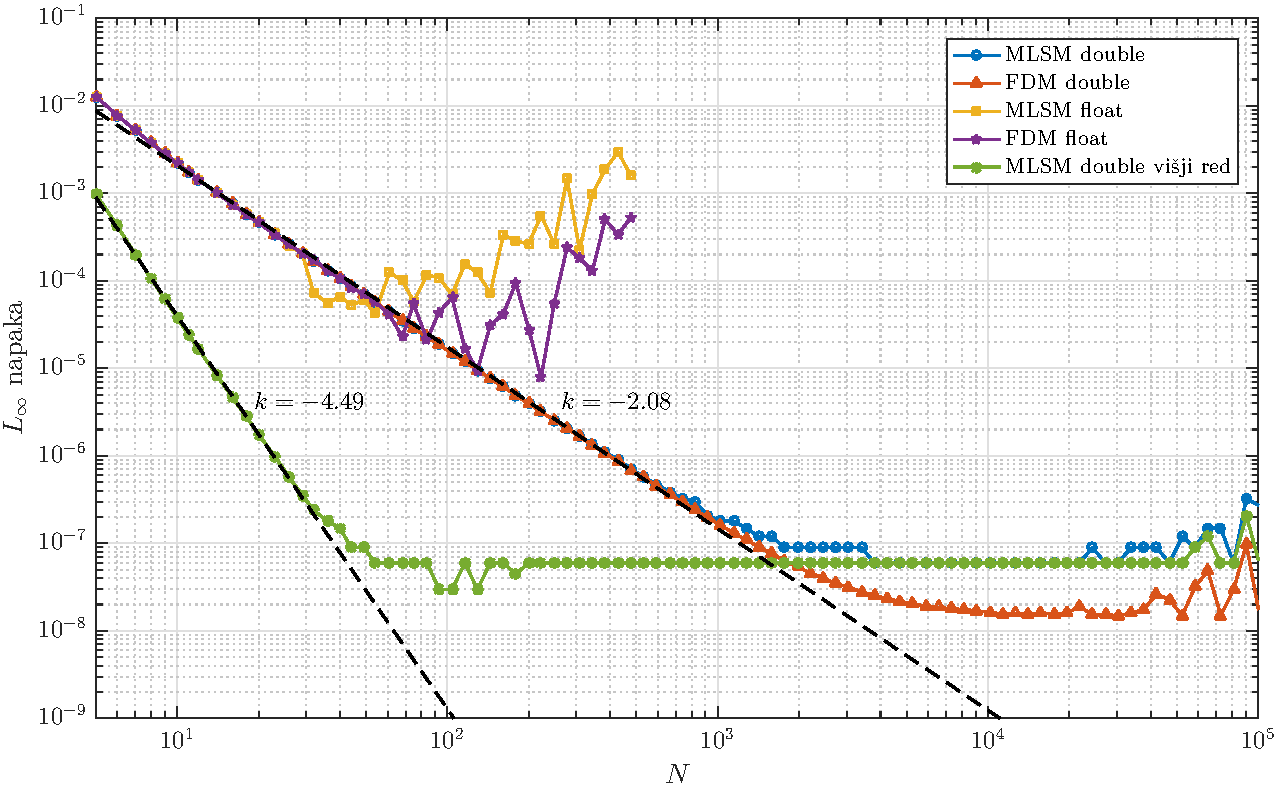
\includegraphics[width=\iw]{images/lap1d_convergence.pdf}
  \caption[Napaka FDM in MLSM metode.]{Napaka FDM in MLSM metode v primerjavi s pravilno rešitvijo.}
  \label{fig:mlsm-fdm-err}
\end{figure}

Na grafu (slika~\ref{fig:mlsm-fdm-err}) vidimo, da metodi tudi v praksi sovpadata dokler ne preideta
v območje nestabilnosti. Pri enojni natančnosti se to zgodi precej hitro, pri $N = 30$, pri dvojni
natančnosti pa obe metodi konvergirata linearno do približno $N = 1000$. Nato se obe metodi
približujeta vsaka svoji največji možni natančnosti, med $N = 10^4$ in $N = 10^5$ diskretizacijskimi
točkami pa se začnejo pojavljati numerične nestabilnosti. Manjšo končno natančnost MLSM lahko
pripišemo numeričnim napakam pri računanju aproksimacije drugih odvodov. Pri FDM namreč v matriko
direktno zapišemo koeficiente $\frac{1}{h^2}$ in $-\frac{2}{h^2}$, pri MLSM pa se ti izračunajo
numerično. Iz naklona premice vidimo, da sta obe metodi tudi v praksi reda~2. Če uporabimo za
računanje aproksimacije odvoda 5 sosedov namesto 3, po pričakovanjih dobimo metodo, ki konvergira z
višjim redom, ima pa enako končno natančnost kot prej.

\begin{figure}[h]
  \centering
  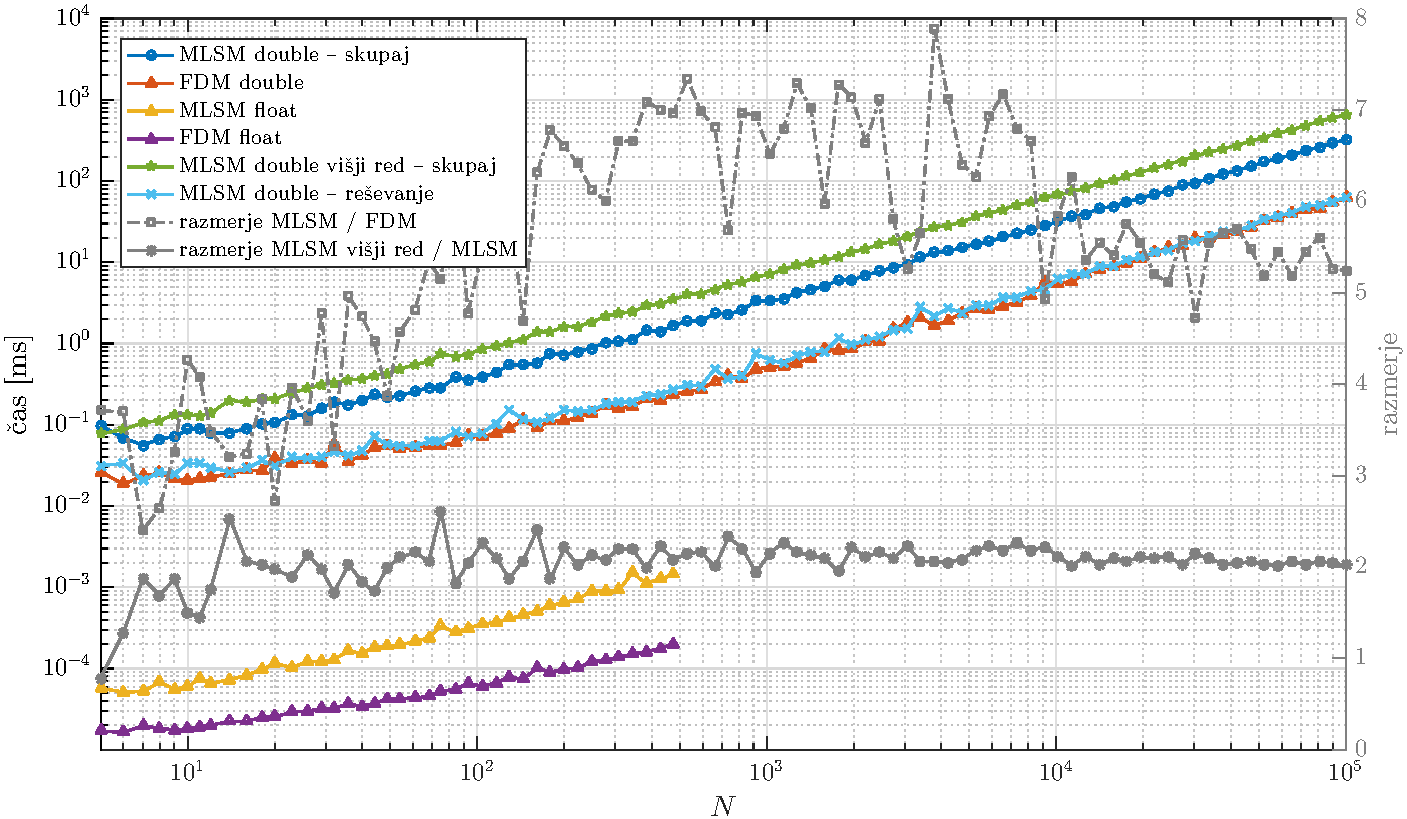
\includegraphics[width=\iw]{images/lap1d_times.pdf}
  \caption{Primerjava časa izvajanja MLSM in FDM metod.}
  \label{fig:mlsm-fdm-time}
\end{figure}

Časovna primerjava obeh metod je prikazana na sliki~\ref{fig:mlsm-fdm-time}. MLSM je približno
konstantno 5.5-krat počasnejši kot FDM za velike $(\geq 10^4)$ $N$, kot prikazano z razmerjem,
merjenim na desni osi. To je tudi pričakovano, saj MLSM išče sosede in gradi funkcije oblike, medtem
ko so uporabljene aproksimacije pri FDM znane vnaprej. Če pri MLSM posebej merimo samo čas, ki ga
porabimo za sestavljanje matrike in reševanje sistema, vidimo, da se skoraj ujema z časom,
porabljenim pri FDM. Majhno razliko gre pripisati razliki pri načinu grajenja matrike, saj pri FDM
natanko vemo pozicije in število neničelnih elementov vnaprej, medtem ko za MLSM to v splošnem ne
velja. MLSM višjega reda je pričakovano počasnejši saj sta $n$ in $m$ poleg osnovnega faktorja $N$
glavna parametra v časovni zahtevnosti~\eqref{eq:casovna-zahtevnost}. Iz razmerja vidimo, da je MLSM
višjega reda konsistentno dvakrat počasnejša. Toda, če pogledamo koliko časa potrebujemo, da
dosežemo natančnost $10^{-6}$, z grafov~\ref{fig:mlsm-fdm-err} in~\ref{fig:mlsm-fdm-time} odčitamo,
da MLSM višjega reda potrebuje le $N = 22$ točk, za kar potrebujemo $\unit[0.3]{ms}$, pri običajnem
redu pa potrebujemo $N = 400$ točk, kar nanese $\unit[1.5]{ms}$. Implementacija deljenih diferenc
višjega reda je dovolj zoprna, da se zanjo malokrat odločimo, saj je treba uporabljati enostranske
diference pri robu. Pri MLSM pa se izračunajo same, vse kar je potrebno je, da $n$ iz 3 spremenimo
na 5. Če uporabljamo enojno natančnost namesto dvojne, se to zgolj malenkostno pozna na času, ki ga
porabimo za reševanje, in se zaradi njene zgodnje nestabilnosti enojne natančnosti ne splača uporabljati.

\subsection{Poissonova enačba}
Oglejmo si obnašanje numerične rešitve klasične Poissonove enačbe na kvadratu:
\begin{align}
  \lap u &= 1, \quad (x, y) \in (0, 1) \times (0, 1)
  \label{eq:poisson-problem} \\
  u(x, 0) &= u(x, 1) = u(0, y) = u(1, y) = 0. \nonumber
\end{align}
Analitično rešitev lahko dobimo s pomočjo separacije spremenljivk in se glasi
\begin{equation}
  u(x, y) =
  -8 \sum_{\substack{k=1 \\ k \text{ lih}}}^\infty \frac{ \sin (k \pi  x) \sinh
  \frac{k \pi  (1-y)}{2} \sinh \frac{k \pi
y}{2}}{\cosh(\frac{k\pi}{2})k^3 \pi ^3}.
  \label{eq:poisson-analytical}
\end{equation}
Za primerjavo z numeričnimi rešitvami bomo uporabili končno vsoto, zato ocenimo
ostanek.
\begin{trditev}
  Za ostanek vrste~\eqref{eq:poisson-analytical} velja
  \begin{equation}
    \left|-8 \sum_{\substack{k=\ell \\ k \text{ lih}}}^\infty \frac{ \sin (k \pi  x) \sinh
      \frac{k \pi  (1-y)}{2} \sinh \frac{k \pi y}{2}}{\cosh(\frac{k\pi}{2})k^3
      \pi ^3}\right| < -\frac{\psi''(\ell/2)}{4 \pi^3},
  \end{equation}
  kjer je $\psi(x) = \ddx{}\log\Gamma(x)$ digama funkcija.
\end{trditev}
\begin{proof}
Ocenjujmo vsak člen vrste posebej. Funkcijo $\sin$ ocenimo z 1, funkcija
$\sinh \frac{k \pi  (1-y)}{2} \sinh \frac{k \pi y}{2}$ ima maksimum na sredini
intervala in jo lahko ocenimo z njeno vrednostjo v $y = \frac{1}{2}$.
Tako nam ostane za oceniti številska vrsta
\[
    -8 \sum_{\substack{k=\ell \\ k \text{ lih}}}^\infty
    \frac{\left(\sinh\frac{k \pi}{4}\right)^2}{\cosh(\frac{k\pi}{2})k^3
    \pi ^3} .
\]
Uporabimo še neenakost $\frac{\left(\sinh\frac{k
\pi}{4}\right)^2}{\cosh(\frac{k\pi}{2})} < \frac{1}{2}$ in dobimo oceno
\[
\left|-8 \sum_{\substack{k=\ell \\ k \text{ lih}}}^\infty \frac{ \sin (k \pi  x) \sinh
      \frac{k \pi  (1-y)}{2} \sinh \frac{k \pi y}{2}}{\cosh(\frac{k\pi}{2})k^3
      \pi ^3}\right| < \frac{4}{\pi^3} \sum_{\substack{k=\ell \\ k \text{ lih}}}^\infty
      \frac{1}{k^3} = -\frac{\psi''(\ell/2)}{4 \pi^3},
\]
kjer je $\psi$ digama funkcija (in posledično $\psi''$ poligama funkcija).
\end{proof}
Za primer $\ell = 1$  v prejšnji trditvi dobimo oceno
\begin{equation}
   |u(x, y)| \leq \frac{7 \zeta(3)}{2 \pi^2} \approx 0.1356,
\end{equation}
kar drži; v resnici je najbolj ekstremna vrednost $u(1/2, 1/2) \approx -0.0736$.
Iz zgornje trditve lahko izračunamo, da je rep
vrste~\eqref{eq:poisson-analytical} za $\ell = 59$ manjši kot $10^{-5}$, za
$\ell = 181$ pa manjši kot $10^{-6}$. Za izračun analitične rešitve ob
primerjavi z numerično je uporabljen $\ell = 181$.
\begin{opomba}
  Računanje izraza
  \begin{equation}
   \frac{\sinh \frac{k \pi  (1-y)}{2} \sinh \frac{k \pi y}{2}}{\cosh(\frac{k\pi}{2})}
  \end{equation}
  ni numerično stabilno, ko $k$ raste, kajti tako števec kot imenovalec se približujeta
  neskončnosti, kvocient pa ima končno limito. Ko ga želimo izračunati numerično je bolje uporabiti
  stabilnejšo obliko
  \begin{equation}
    \frac12\left( 1 - \frac{\exp(-k\pi y) + \exp(-k\pi(1-y)) }{1 + \exp(-k\pi)}\right),
  \end{equation}
  kjer vedno nastopa negativen eksponent.
\end{opomba}

Rešimo problem~\eqref{eq:poisson-problem} numerično, s štirimi različnimi nabori baznih funkcij:
monomi, Gaussovimi funkcijami~(G), multikvadratičnimi~(MQ) in inverznimi multikvadratičnimi~(IMQ).
Za parametre smo vedno vzeli $n = m = 9$ kar sovpada s primeri iz
razdelka~\ref{sec:posebni-primeri}. Pri monomih smo dodali tudi primer $n = 9$ in $m = 6$. Za
parameter oblike pri radialnih baznih funkcijah smo vzeli $\sigma_b = 100\, r_\chi$. Za utež
vzemimo Gaussovo utež z $\sigma_w = \frac34 r_\chi$. V vseh primerih je bila za reševanje sistema
enačb uporabljena direktna metoda SuperLU.\footnote{Iterativni BiCGSTAB algoritem je vrnil enake
rezultate.} Primerjava napak je prikazana na sliki~\ref{fig:poisson-square-convergence}.

\begin{figure}[h]
  \centering
  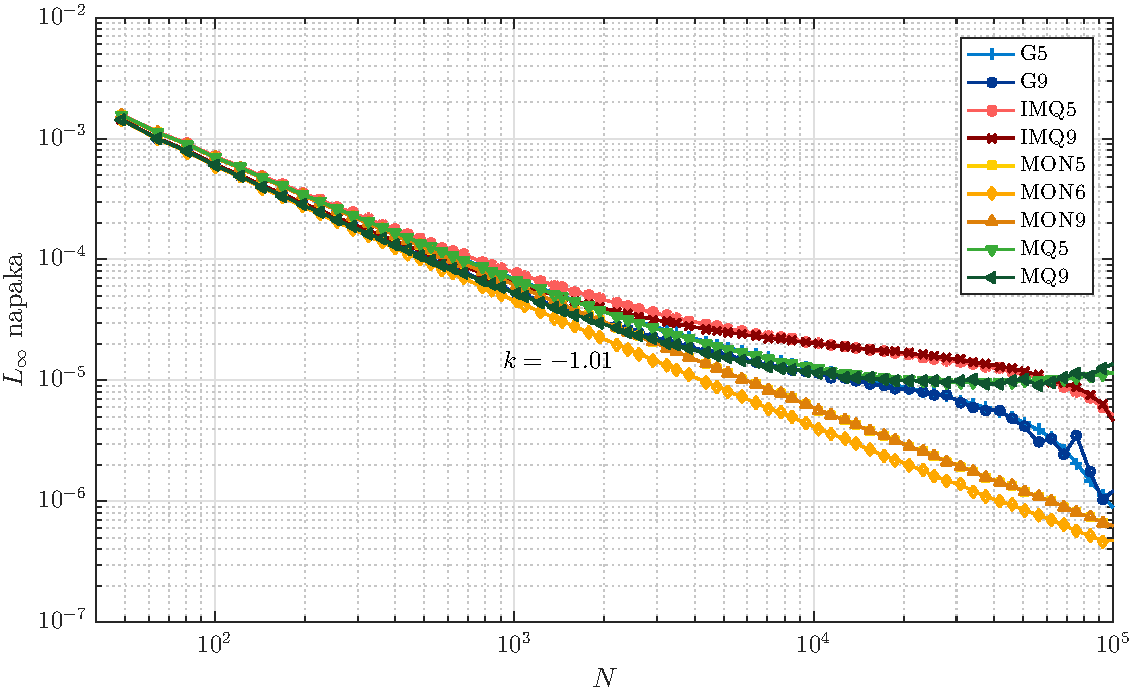
\includegraphics[width=\iw]{images/poisson_square_convergence.pdf}
  \caption[Konvergenca MLSM pri reševanju Poissonove enačbe]{Konvergenca MLSM
  za različne parametre pri reševanju problema~\eqref{eq:poisson-problem}.}
  \label{fig:poisson-square-convergence}
\end{figure}

Vidimo, da monomi za $n=5$ in $n=9$ konvergirajo linearno z redom 2 (glede na $\sqrt{N}$), kar vemo
tudi iz teorije metode končnih diferenc. Radialne bazne funkcije se na začetku ujemajo z monomi,
nato pa pokažejo slabše konvergenčne lastnosti in nelinearno obnašanje, drugačno pri vsakem razredu
funkcij. Funkcije, ki uporabljajo več sosedov, začnejo z malenkost nižjo napako, prav tako pa morda
presenetljivo tudi monomi z $n=6$. S slike~\ref{fig:poisson-square-time}, ki prikazuje čas
računanja, vidimo, da se uporaba baznih funkcij z $n = 9$ ne splača, saj minimalna pridobljena
natančnost ne odtehta časa izvajanja. Vidimo, da se čas izvajanja loči na tri pasove glede na $n$,
ki vsi rastejo linearno z $N$ s konstantnim razmerjem.

\begin{figure}[h]
  \centering
  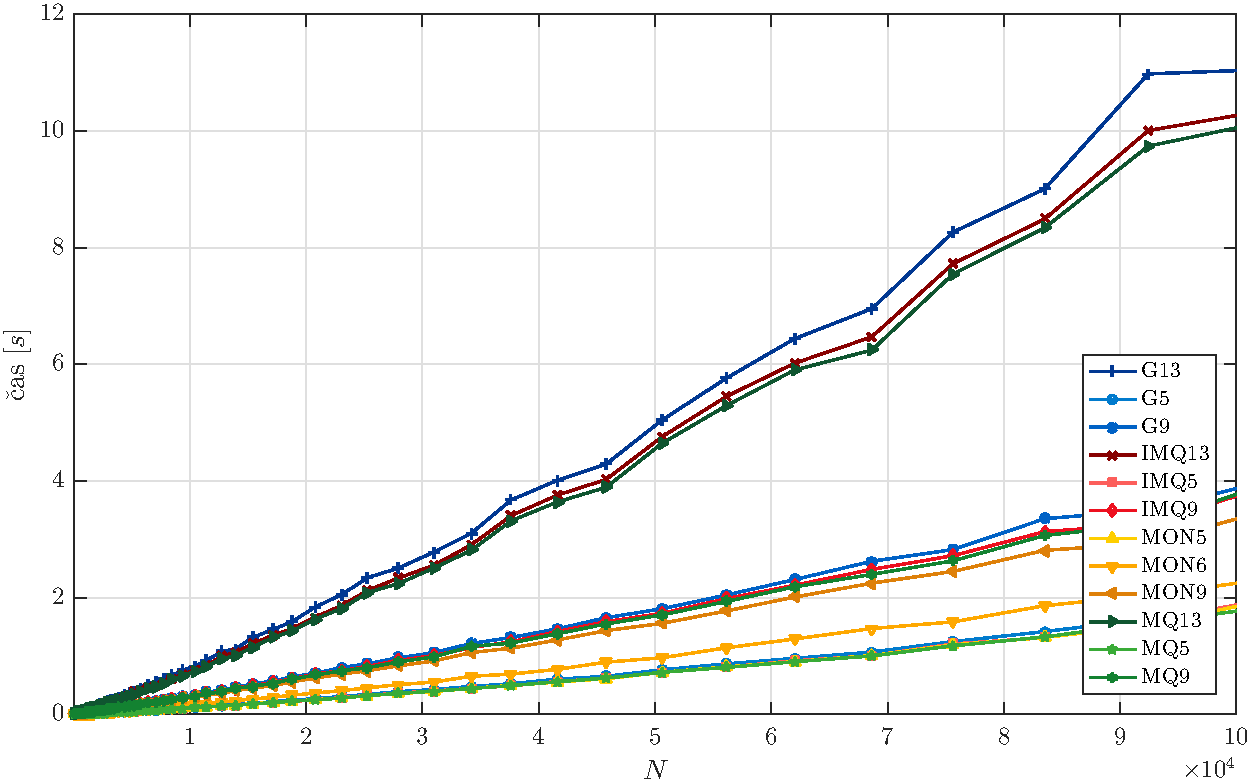
\includegraphics[width=\iw]{images/poisson_square_time.pdf}
  \caption[Čas izvajanja MLSM pri reševanju Poissonove enačbe]{Čas izvajanja za
  različne izbore parametrov pri reševanju
problema~\eqref{eq:poisson-problem}.}
  \label{fig:poisson-square-time}
\end{figure}

Po trditvi~\ref{trd:rbf-konv-k-mon} aproksimacija z Gaussovimi funkcijami konvergira proti
aproksimaciji z monomi. Slika~\ref{fig:rbf-konv-k-mon} to dejstvo potrjuje. Konvergenčne krivulje za
Gaussove funkcije se pri povečevanju parametra oblike čedalje bolj približujejo konvergenčni
krivulji monomov. Če imamo pri radialnih baznih funkcijah težavo s konvergenco, lahko poizkusimo
povečati parameter oblike. Seveda to ne gre prek vseh meja, saj sistem~\eqref{eq:shape-system} za
izračun funkcije oblike z večanjem parametra oblike postane čedalje bolj občutljiv.

\begin{figure}[h]
  \centering
  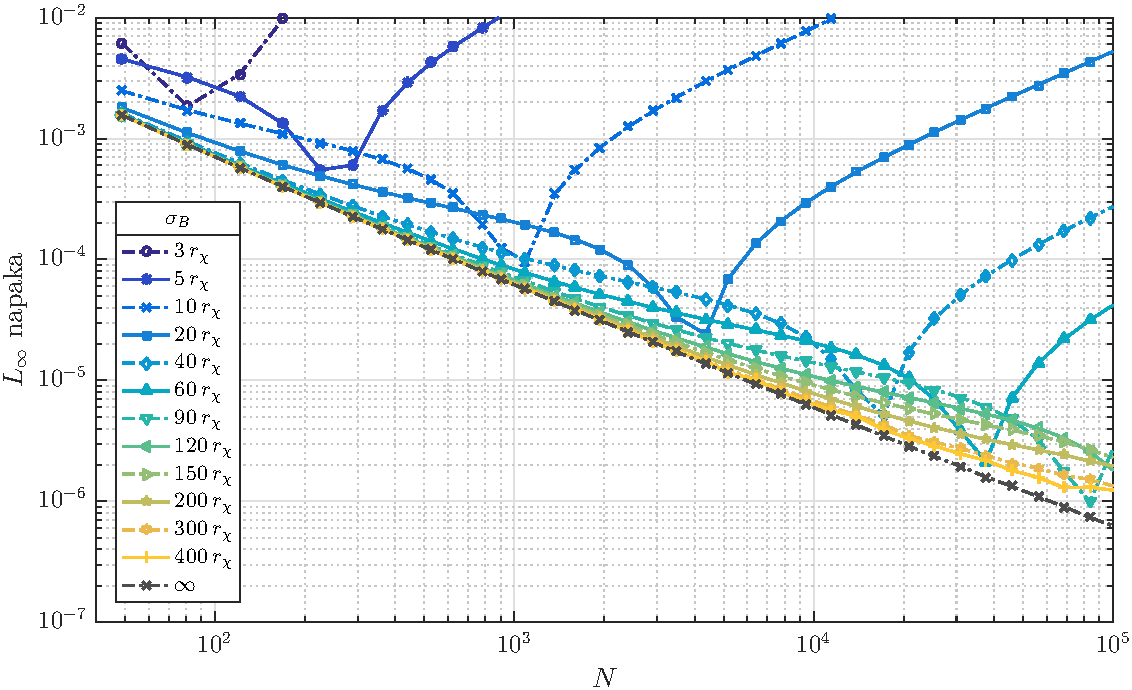
\includegraphics[width=\iw]{images/poisson_square_rbf_konv_k_mon.pdf}
  \caption[Konvergenčne krivulje za Gaussove funkcije.]{Konvergenčne krivulje
  za Gaussove funkcije pri čedalje večjem $\sigma$ in za monome ($\sigma =
  \infty$). Uporabili smo $n = m = 5$ in Gaussovo utež s parametrom $\sigma_w =
  \frac34 r_\chi$.}
  \label{fig:rbf-konv-k-mon}
\end{figure}

Da si izboljšamo intuicijo o pomenu parametrov oblike pri uporabi radialnih
baznih funkcij in uteži naredimo še eno analizo, ki nam bo pomagala pri izbiri
parametrov pri bolj zapletenih problemih. Problem~\eqref{eq:poisson-problem}
rešimo za različne izbire parametrov oblike baznih funkcij ($\sigma_b$) in
Gaussove funkcije uteži ($\sigma_w$) ter primerjajmo natančnost rešitve.
Graf napake je prikazan na sliki~\ref{fig:poisson-square-sigma-dep-error}.

\begin{figure}[h]
  \centering
  \begin{subfigure}[t]{0.45\textwidth}
    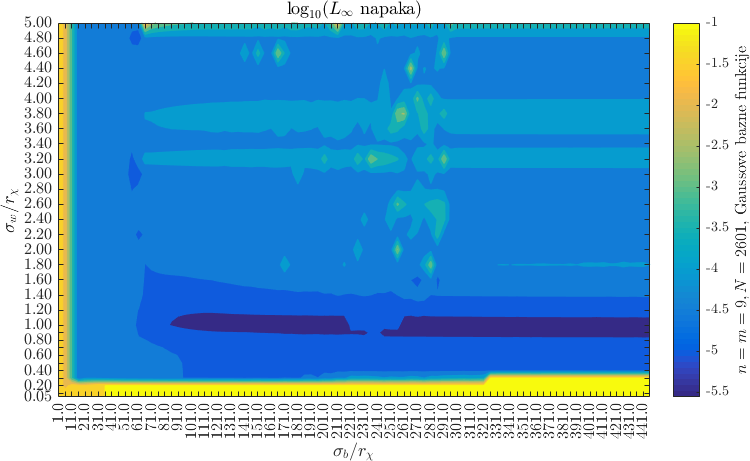
\includegraphics[width=\textwidth]{images/poisson_square_sigma_depedence_error.png}
    \caption{Napaka v odvisnosti od $\sigma_b$ in $\sigma_w$.}
    \label{fig:poisson-square-sigma-dep-error}
  \end{subfigure}
  \begin{subfigure}[t]{0.45\textwidth}
    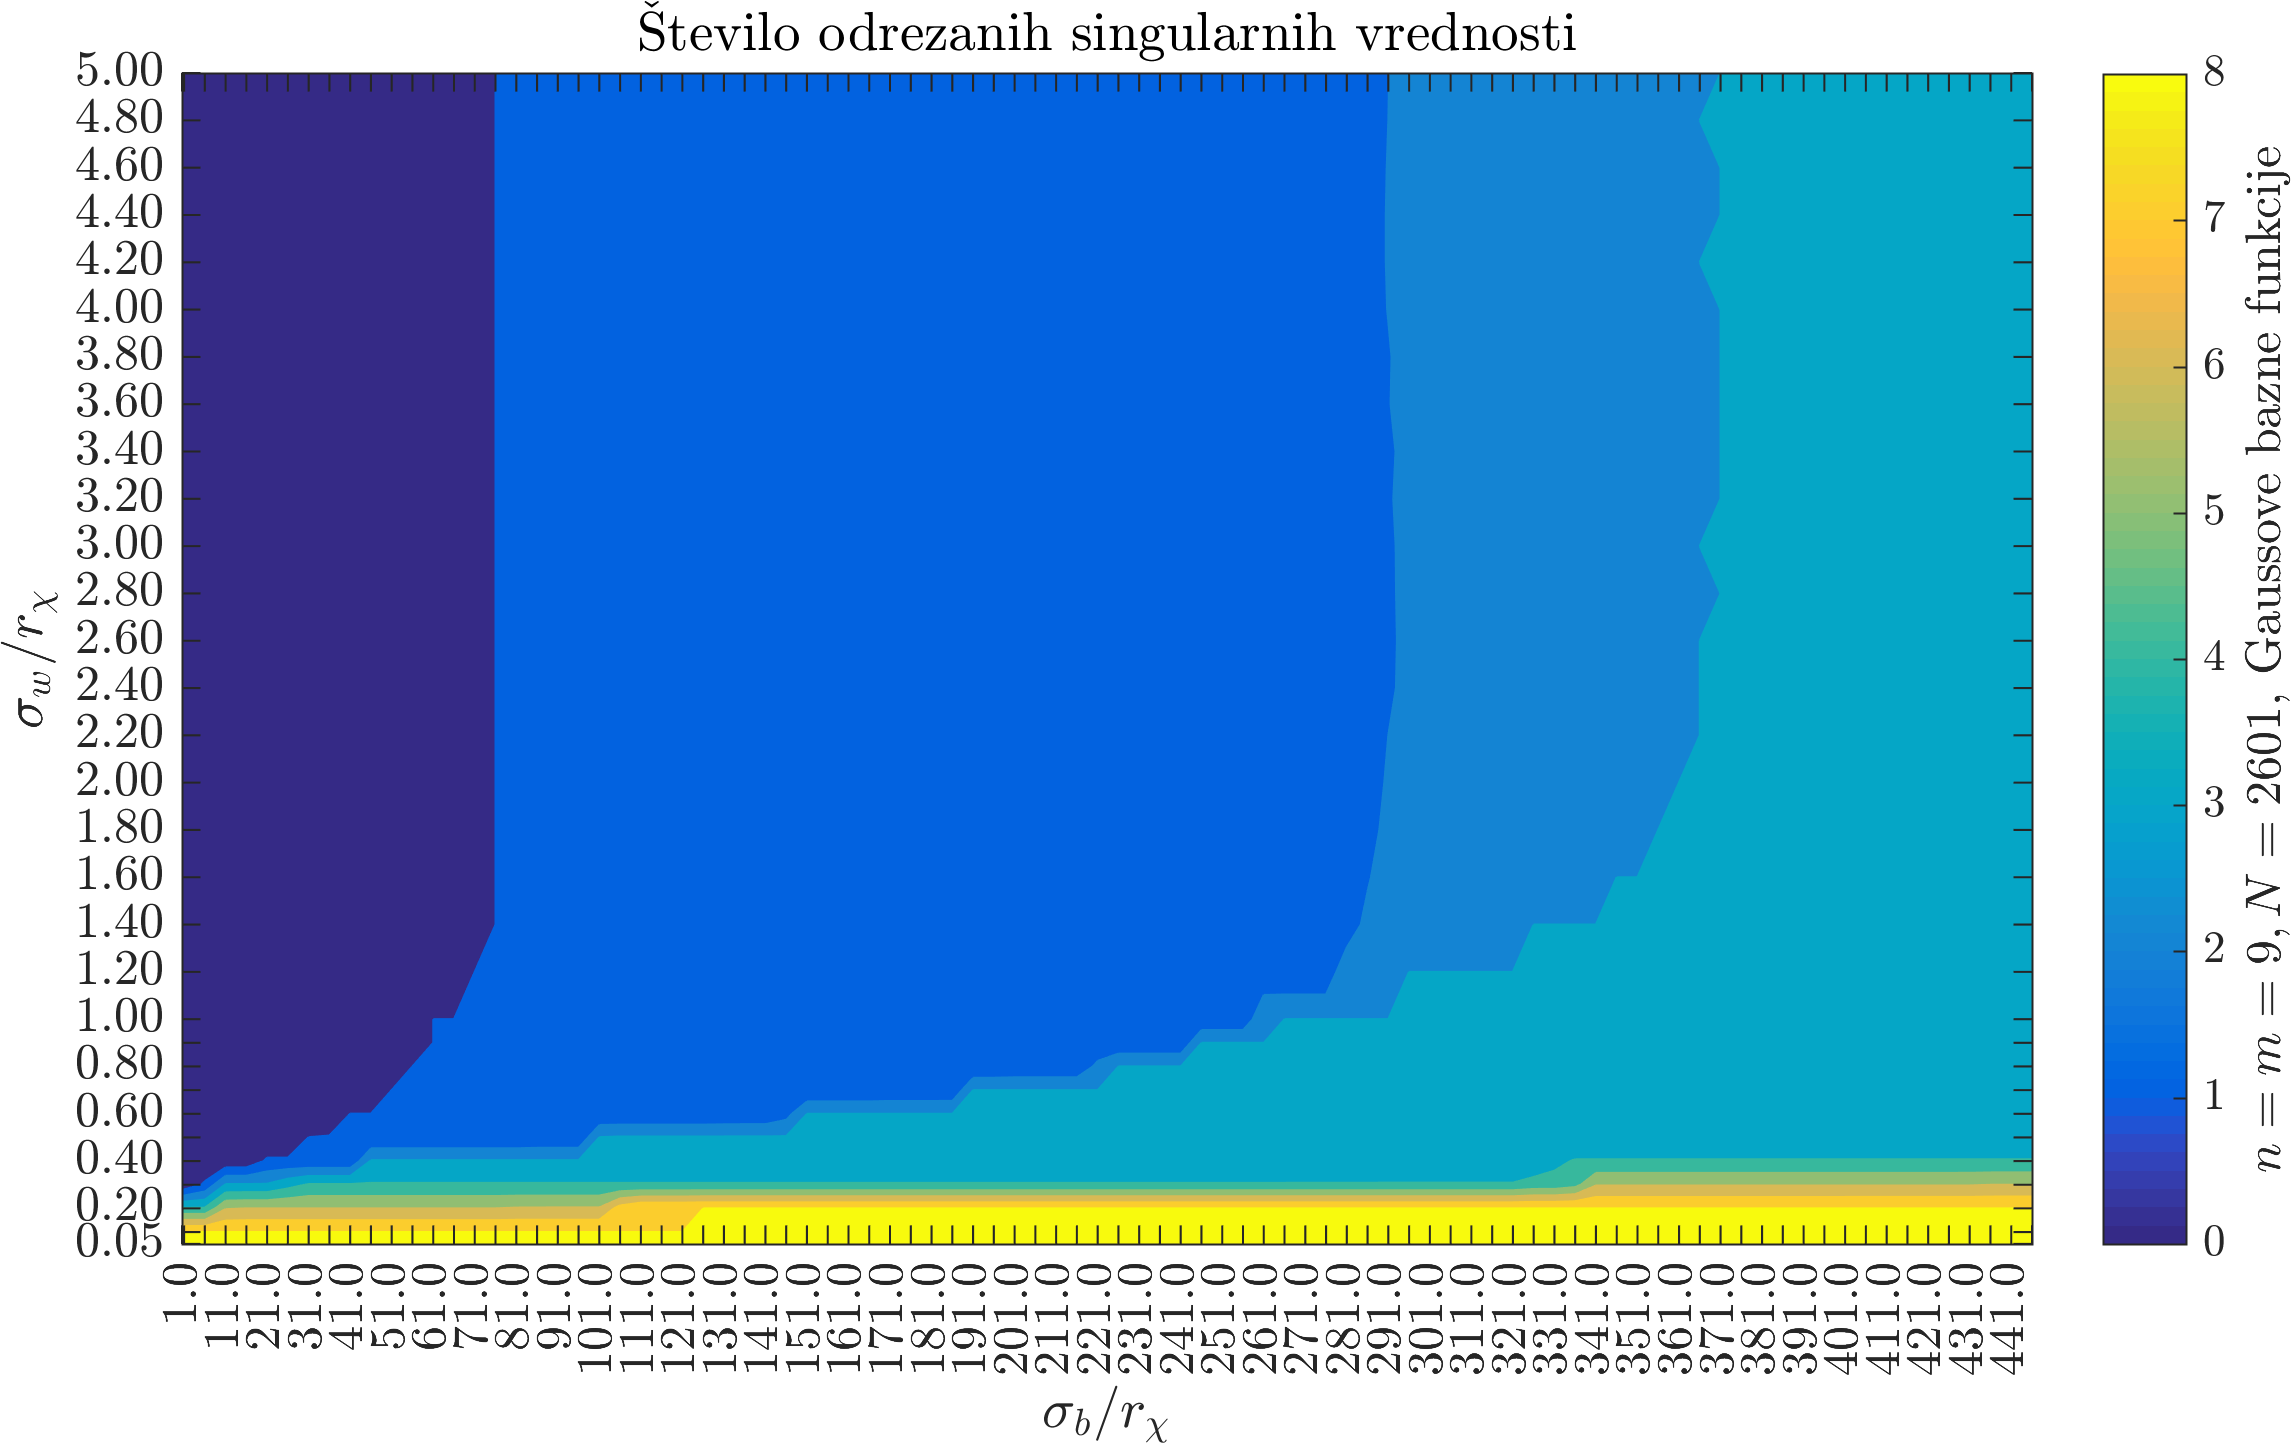
\includegraphics[width=\textwidth]{images/poisson_square_sigma_depedence_cutoff.png}
    \caption[Število odrezanih singularnih vrednosti.]{Število odrezanih
    singularnih vrednosti v odvisnosti od $\sigma_b$ in $\sigma_w$.}
    \label{fig:poisson-square-sigma-dep-cutoff}
  \end{subfigure}
  \caption[Reševanja Poissonove enačbe z Gaussovimi funkcijami in utežjo.]{Analiza reševanja
  problema~\eqref{eq:poisson-problem} z Gaussovimi funkcijami in Gaussovo utežjo pri $n = m = 9$ in
  $N = 2601$.}
  \label{fig:poisson-square-sigma-dep}
\end{figure}

Trditev~\ref{trd:weight-independence} pravi, da mora biti v primeru $n=m$ in obrnljive matrike $B$
aproksimacija operatorja (in posledično tudi napaka) neodvisna od izbire uteži. Opomba po trditvi
pravi, da numerično to velja, če le utež ni premajhna, da bi bila sama razlog za numerične
nestabilnosti. Slika~\ref{fig:poisson-square-sigma-dep-error} to potrdi; trditev velja v območju,
kjer je matrika tudi numerično obrnljiva. Če je utež zelo majhna, manjša od $0.3\,r_\chi$, potem se
nekatere enačbe v sistemu~\eqref{eq:shape-system} pomnožijo s približno $\exp(-2/0.3^2) \approx
2.23\cdot10^{-10}$, kar privede do velike nestabilnosti. Do numerične neobrnljivosti matrike pa
lahko pripelje tudi izbira prevelikega parametra $\sigma_b$, kajti za $\sigma_b = 70\,r_\chi$ so vsi
elementi matrike $B$ med $1.00041$ in $1$. Boljši vpogled v obrnljivost matrike $B$ nam da graf na
sliki~\ref{fig:poisson-square-sigma-dep-cutoff}, ki predstavlja število odrezanih singularnih
vrednosti pri SVD razcepu, s pomočjo katerega smo izračunali psevdoinverz matrike $WB$.
Aproksimacija je res neodvisna od uteži na predelu, kjer nismo odrezali nobene singularne vrednosti,
torej približno na območju $[0, 70] \times [0.3, \infty)$, drugje pa lahko utež vpliva na izračun
psevdoinverza in število odrezanih singularnih vrednosti.

Kvaliteta aproksimacije je za $\sigma_b$ blizu 0 zelo slaba, saj imajo bazne funkcije neničelno
vrednost samo v svojem centru. Nato napaka pada z večanjem $\sigma_b$, dokler ne pridemo v območje
numerične neobrnljivosti matrike $B$. Tam pride v igro regularizacija v SVD razcepu, ki nam lahko
pomaga, kot lahko to vidimo v pasu nizke napake okoli $\sigma_w = 1$. Na
sliki~\ref{fig:poisson-square-sigma-dep-cutoff} vidimo, da se z večanjem $\sigma_b$ reže čedalje več
singularnih vrednosti in sčasoma bi aproksimacija zopet postala nestabilna. Podobno sliko dobimo
pri različnih $N$, $n$ in ostalih izbirah baznih funkcij. Običajno zato izberemo sorazmerno velik
parameter $\sigma_b$ okoli $150\,r_\chi$, za obliko uteži pa vzamemo približno $r_\chi$.

V dosedanjih analizah smo videli, da se MLSM metoda obnaša enako ali slabše kot metoda končnih
diferenc na šolskih primerih. Njena prednost leži v splošnosti, saj se jo z lahkoto prilagodi na
drugačne domene, v višje dimenzije in na druge operatorje. Na sliki~\ref{fig:poisson-square-weird}
so prikazane rešitve Poissonove enačbe $\lap u = 1$ s homogenimi robnimi pogoji na bolj zanimivih
domenah in v višjih dimenzijah. V dveh dimenzijah so bili za bazne funkcije uporabljeni monomi $\{1,
x, y, x^2, y^2\}$ in $n=5$ v treh pa 9 Gaussovih baznih funkcij z $\sigma_b = 50\,r_\chi$ in
Gaussovo utežjo s $\sigma_w = r_\chi$ na devetih točkah. V vseh primerih je bilo potrebno poleg
parametrov spremeniti le definicijo domene, ostala formulacija je ostala enaka.

\begin{figure}[h]
  \centering
  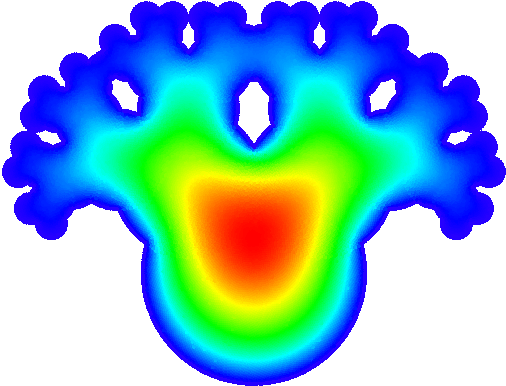
\includegraphics[height=5cm]{images/poisson_weird1.png}
  \hspace{10pt}
  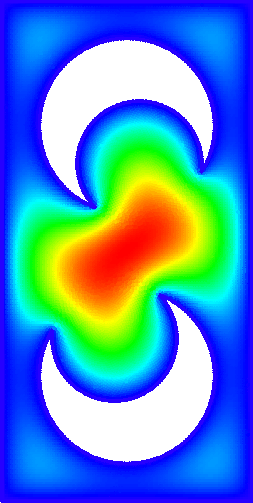
\includegraphics[height=5cm]{images/poisson_weird2.png}
  \hspace{10pt}
  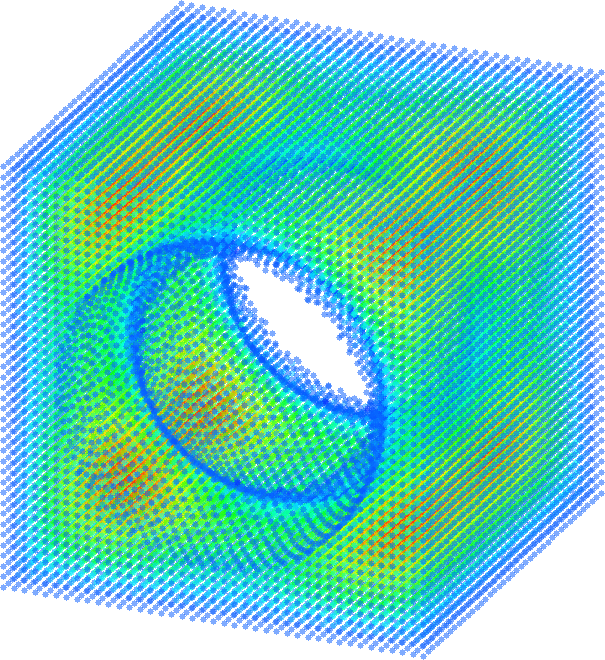
\includegraphics[height=5cm]{images/poisson_weird3.png}
  \caption[Reševanje $\lap u = 1$ na zanimivejših domenah.]{Reševanje Poissonove enačbe $\lap u = 1$ s homogenimi robnimi pogoji na
  zanimivejših domenah.}
  \label{fig:poisson-square-weird}
\end{figure}

\subsection{Vpet nosilec}
Problem vpetega nosilca \ang{cantilever beam} je standarden problem v linearni elastomehaniki in eden
osnovnih testnih primerov za raziskovanje obnašanja numeričnih metod. Imejmo tanek nosilec dolžine
$L$ in višine $D$ vpet na desnem koncu, ki ga na levem koncu potiska navzdol sila $P$ na enoto
debeline. Idealizirana Timoshenkova teorija nosilcev nudi analitično rešitev za ta problem v primeru
predpostavke o ravninski napetosti. Napetosti v nosilcu, ki smo ga postavili na območje $[0, L]
\times [-D/2, D/2]$ so izpeljane v~\cite[str.\ 284--289, enačba 7.4.55]{slaughter2012linearized} in
se izražajo kot
\begin{align}
  \ts_{xx} &= \frac{Pxy}{I}, \quad \ts_{yy} = 0, \quad \ts_{xy} = \frac{P}{2I} \left( \frac{D^2}{4}
  - y^2 \right),
  \label{eq:cantilever-beam-analytical-stress}
\end{align}
pomiki pa kot
\begin{align}
  u &= \frac{P y \left(3 D^2 (\nu +1)-4 \left(3 L^2+(\nu +2) y^2-3 x^2\right)\right)}{24 E I}
  \label{eq:cantilever-beam-analytical-u} \\
  v &= -\frac{P \left(3 D^2 (\nu +1) (L-x)+4 (L-x)^2 (2 L+x)+12 \nu  x y^2\right)}{24 E I}, \label{eq:cantilever-beam-analytical-v}
\end{align}
pri čemer je $I = \frac{1}{12} D^3$ vztrajnostni moment preseka nosilca za vrtenje okoli središča,
$E$ Youngov modul in $\nu$ Poissonovo razmerje. Rešimo primer tudi numerično. Rešimo Navierovo
enačbo~\eqref{eq:navier-stac} na $\Omega = [0, L] \times [-D/2, D/2]$ s predpisanim pomikom pri $x =
L$ danim z analitično
rešitvijo~(\ref{eq:cantilever-beam-analytical-u}--\ref{eq:cantilever-beam-analytical-v}). Zgornji
in spodnji rob naj bosta prosta ($\vt = 0$) na levem robu pa vzemimo navpično parabolično
razporejeno silo $\vt = \ts_{xy}\vj$, dano z analitično
rešitvijo~\eqref{eq:cantilever-beam-analytical-stress}.


Z razliko primera pri izpeljavi metode v razdelku~\ref{sec:splosna-izpeljava}, kjer je bila neznana
količina skalarno polje, je tokrat neznana količina vektorsko polje. V tem primeru je
najenostavnejši pristop k rešitvi, da obravnavamo enačbo za vektorsko polje kot posamezne sklopljene
enačbe za komponente polja, ki so skalarne funkcije. Oglejmo si postopek na primeru dvodimenzionalne
Navierove enačbe. Vektorsko polje razpišemo po komponentah, za primer dveh dimenzij zapišemo $\vu =
(u, v)$. Vektorska oblika stacionarne Navierove enačbe
\begin{equation}
  (\lambda+\mu)\nabla(\nabla\cdot \vu) + \mu\nabla^2 \vu + \vf = 0
\end{equation}
se razpiše v sistem dveh enačb
\begin{align}
  \label{eq:navier-components-1}
(\lambda +\mu ) \left(\dpar{^2u}{x^2}+\dpar{^2v}{xy}\right)+\mu  \left(\dpar{^2u}{x^2}+\dpar{^2u}{y^2}\right)+f_1&=0 \\
(\lambda +\mu ) \left(\dpar{^2u}{xy}+\dpar{^2v}{y^2}\right)+\mu  \left(\dpar{^2v}{x^2}+\dpar{^2v}{y^2}\right)+f_2&=0
\end{align}
Enačbe so sklopljene preko operatorja $\grad\div$. Če domeno diskretiziramo z $N$ točkami, bomo
namesto sistema $N\times N$ za neznano skalarno polje, sedaj reševali sistem $2N\times 2N$ za
obe skalarni polji hkrati. Neznanke, ki ustrezajo vektorju $\vu$ predstavimo numerično kot vektor
$\b{u}$ dolžine $2N$, katerega prvih $N$ komponent predstavlja $u$, preostalih $N$ pa predstavlja $v$.
Enako storimo z $\vf$ in robnimi pogoji. Enačbo $A\b u = \b f$ lahko sedaj zapišemo po blokih
\begin{equation}
  \begin{bmatrix}
    U1 & V1 \\
    U2 & V2
  \end{bmatrix}
  \begin{bmatrix}
    u \\ v
  \end{bmatrix}
  =
  \begin{bmatrix}
    f_1 \\ f_2
  \end{bmatrix}.
  \label{eq:higher-dim-system}
\end{equation}
Vsako izmed komponent Navierove enačbe napišemo v eno izmed (bločnih) vrstic. Funkcijo
oblike za člen $\dpar{^2v}{xy}$ napišemo v blok $V1$, saj nastopa v prvi enačbi in se nahaja v drugi
izmed enačb. Podobno aproksimacijo za $\dpar{^2u}{y^2}$ iz~\eqref{eq:navier-components-1} napišemo
v blok $U1$. Če katere elemente napišemo na mesta, kjer so že kakšni neničelni elementi, jih med
seboj seštejemo. Primer matrike sistema~\eqref{eq:higher-dim-system} je prikazan na
sliki~\ref{fig:cantilever-beam-matrix}. Vidimo, da ima bločno strukturo, kot opisano
v~\eqref{eq:higher-dim-system}, pri čemer se dodatno znotraj blokih vidijo še različni vzorci na
območjih, ki pripadajo notranjim točkam ali točkam na robu.

\begin{figure}[!h]
  \centering
  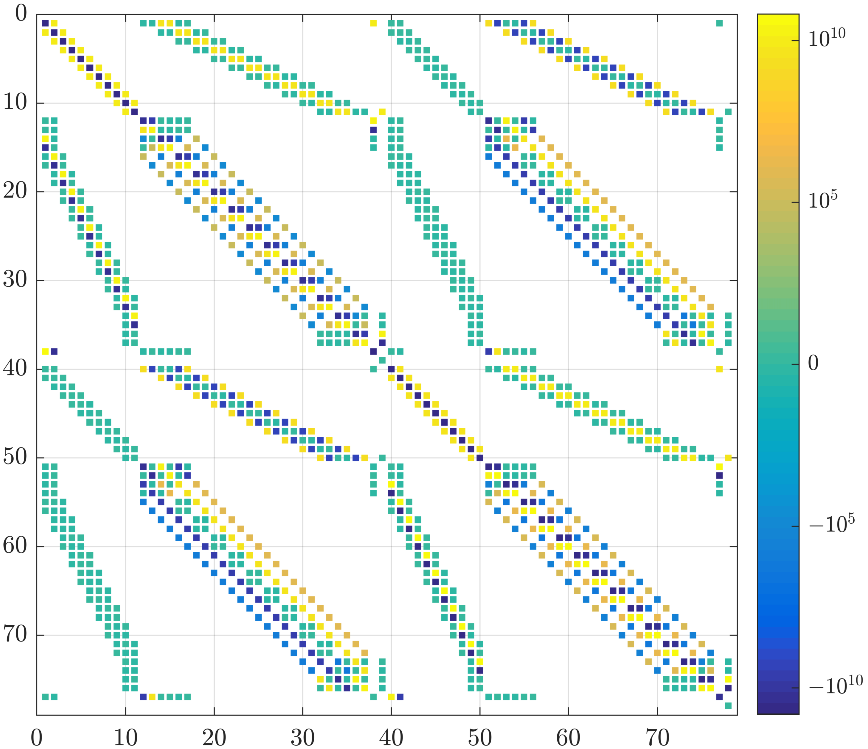
\includegraphics[width=0.6\textwidth]{images/cantilever_beam_matrix_example.pdf}
  \caption[Matrika sistema enačb pri reševanju problema vpetega
  nosilca.]{Matrika končnega sistema enačb~\eqref{eq:higher-dim-system} pri
  reševanju problema vpetega nosilca z 9 monomi in pravokotno
  diskretizacijo z $N = 39$ točkami}
  \label{fig:cantilever-beam-matrix}
\end{figure}

Problem rešimo numerično z uporabo 9 monomov in 9 Gaussovih baznih funkcij z $\sigma_b =
500\,r_\chi$, obakrat z Gaussovo utežjo $\sigma_w = r_\chi$.
Linearni sistem enačb rešimo z iterativnim BiCGSTAB postopkom z ILUT predpogojevanjem
kot opisano v razdelku~\ref{sec:solve-sparse}. Uporabili smo parametra $p=20$ in $\tau = 10^{-5}$.
BiCGSTAB algoritem iteriramo največ 300-krat ali dokler ni ocena napake pod $10^{-13}$.
Algoritem je v vseh primerih konvergiral.

Za parametre problema smo izbrali $L = \unit[30]{m}$, $D = \unit[5]{m}$, $E = \unit[72.1]{GPa}$,
$\nu = 0.33$, $P = \unit[1000]{N/m}$. Numerična rešitev je prikazana na
sliki~\ref{fig:cantilever-beam-solution}. Omeniti je treba še, kako iz numerične rešitve $\b{u}$
dobimo aproksimacijo za $\ts$. Komponente $\ts$ so linearne kombinacije odvodov $\vu$, tako da v
vsaki diskretizacijski točki izračunamo funkciji oblike, ki aproksimirata $\dpar{}{x}$ in
$\dpar{}{y}$ in z njuno pomočjo izračunamo $\frac12 (\grad\vu + \grad\vu^\T)$ ter nato preko
Hookovega zakona~\eqref{eq:hooke-isotropic} dobimo $\ts$.

\begin{figure}[h]
  \centering
  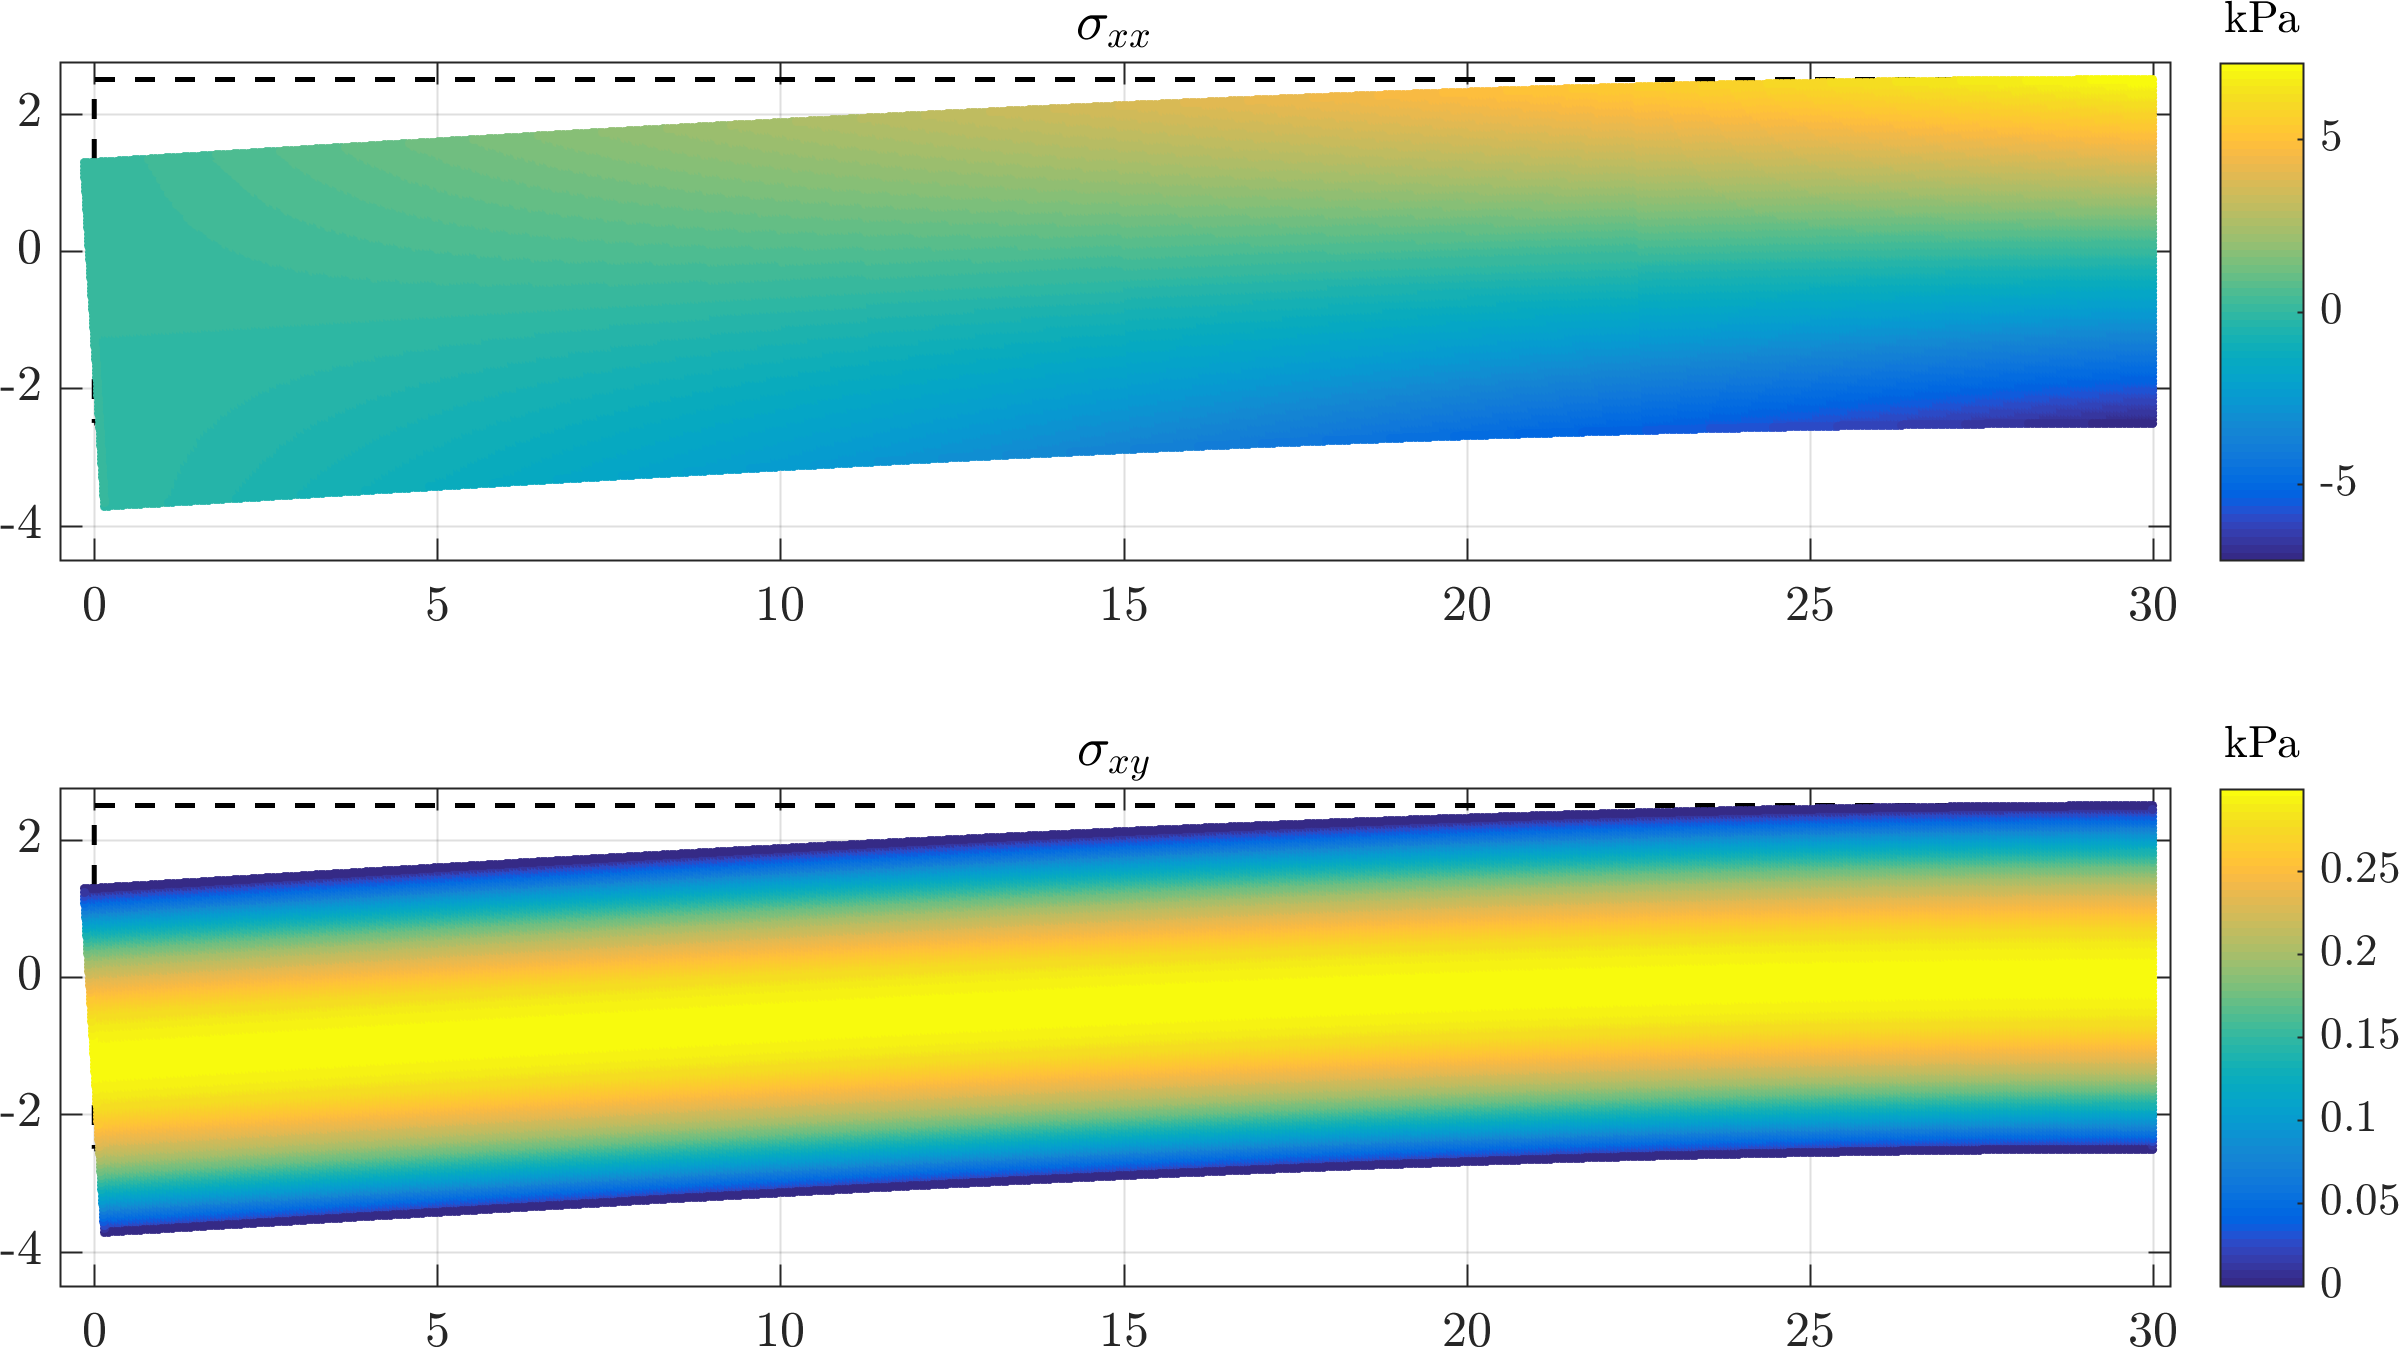
\includegraphics[width=\iw]{images/cantilever_beam_solution.png}
  \caption[Numerična rešitev problema vpetega nosilca.]{Numerična rešitev
  problema vpetega nosilca. Pomiki so zaradi boljše vidnosti povečani za faktor
  $10^5$. Komponenta $\ts_{yy}$ je kot v analitični rešitvi enaka 0.}
  \label{fig:cantilever-beam-solution}
\end{figure}
Izračunajmo še, da je največji pomik
\begin{equation}
  \max_{x \in \Omega} |\vu(x)| \approx \unit[1.22 \cdot 10^{-5}]{m} = \unit[12.2]{\mu m}
\end{equation}
in največji gradient pomika
\begin{equation}
  \max_{x \in \Omega} \|\grad \vu(x)\| \approx 8.53 \cdot 10^{-7}.
\end{equation}
Predpostavka o majhnosti pomikov in njihovih gradientov res velja.

Na sliki~\ref{fig:cantilever-beam-convergence} je prikazana konvergenca numerične rešitve proti
analitični. Napako pomikov in napetosti merimo relativno v $L_\infty$ normi
\begin{align}
  e_\infty(\vu) &= \frac{\max_{x\in \X} \{\max\{|u(x)-\hat u(x)|, |v(x)-\hat v(x)|\}\}}
  {\max_{x\in \X} \{\max\{|u(x)|, |v(x)|\}\}}, \\
  e_\infty(\ts) &= \frac{\max_{x\in \X} \{\max\{|\sigma_{xx}(x)-\hat{\sigma}_{xx}(x)|,
  |\sigma_{yy}(x)-\hat{\sigma}_{yy}(x)|,
  |\sigma_{xy}(x)-\hat{\sigma}_{xy}(x)| \}\}}{
  \max_{x\in \X} \{\max\{|\sigma_{xx}(x)|, |\sigma_{yy}(x)|, |\sigma_{xy}(x)| \}\}}.
\end{align}
kjer s strešico označimo izračunane količine, brez strešice pa analitične.

\begin{figure}[h]
  \centering
  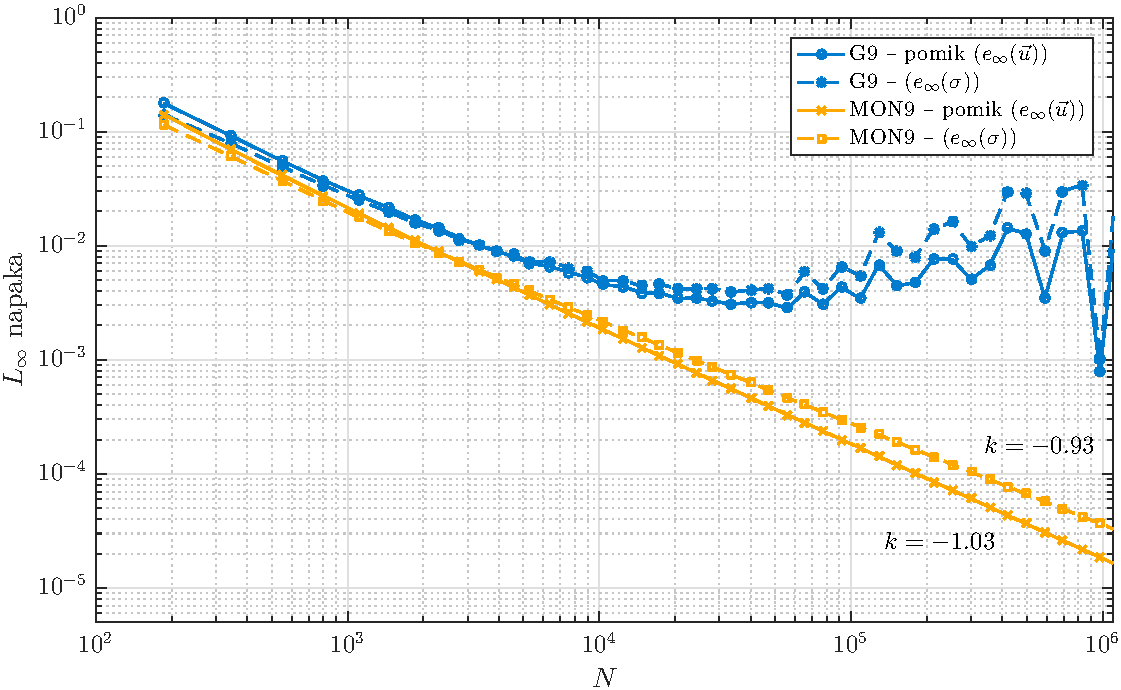
\includegraphics[width=\iw]{images/cantilever_beam_convergence.pdf}
  \caption{Konvergenca numerične metode pri reševanju problema vpetega nosilca.}
  \label{fig:cantilever-beam-convergence}
\end{figure}
Rezultati so podobni kot pri Poissonovi enačbi na sliki~\ref{fig:poisson-square-convergence}.
Monomi konvergirajo zelo regularno z redom $2$, medtem ko z uporabo Gaussovih baznih funkcij
dosegamo nekoliko slabše konvergenčno obnašanje. Vidimo, da konvergirajo tako vrednosti pomikov kot
tudi vrednosti napetosti, pri čemer imamo pri napetostih nekoliko večjo napako in malenkost slabši red,
saj jih ocenjujemo iz pomikov, kaj zahteva še eno diferenčno aproksimacijo več.

Za demonstracijo splošnosti metode dodajmo v nosilec še nekaj lukenj. Nosilec pritrdimo na desnem
koncu ($\vu = 0$) in vlecimo navzdol na levem z enakomerno porazdeljeno silo $P$ enake velikosti kot
prej ($\vt = -P/D\vj$\,). V domeno smo razporedili $N = 177617$ diskretizacijskih točk z večjo
gostoto okoli robov lukenj, po ustvarjanju domene pa smo jo še dodatno izboljšali z
algoritmom~\ref{alg:relax} s 50 iteracijami na šestih sosedih z $F_0 = 10^{-3}$ in $\alpha = 3$.
Upogib nosilca, obarvan z vrednostjo von Misesove napetosti je prikazan na
sliki~\ref{fig:cantilever-beam-with-holes}. Von Misesova napetost se za primer ravninske napetosti
izračuna kot
\begin{equation}
  \sigma_v = \sqrt{\sigma_{xx}^2-\sigma_{xx}\sigma_{yy}+\sigma_{yy}^2+3\sigma_{xy}^2},
\end{equation}
in se uporablja v von Misesovem kriteriju plastičnosti. Ta pravi, da material ni več
elastičen, ko $\sigma_v$ preseže neko materialno konstanto $\sigma_0$. Višje vrednosti $\ts_v$
torej nakazujejo, da je material bližje meji svoje elastičnosti in visoke vrednosti $\ts_v$
označujejo najverjetnejša mesta za poškodbe. Največji pomik v tem primeru je
\begin{equation}
  \max_{x \in \Omega} |\vu(x)| \approx \unit[1.55 \cdot 10^{-5}]{m} = \unit[15.5]{\mu m}.
\end{equation}

\begin{figure}[h]
  \centering
  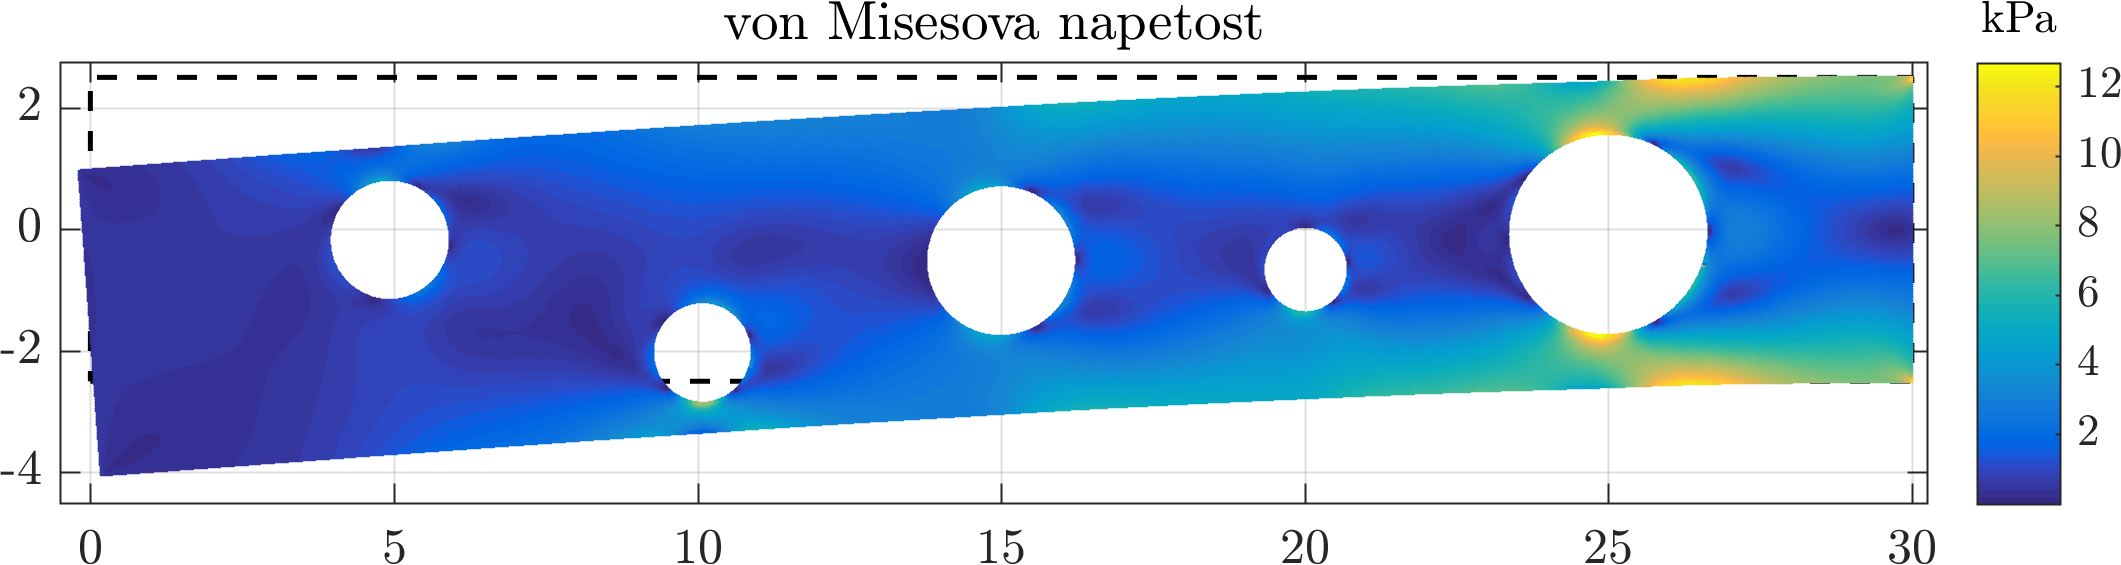
\includegraphics[width=0.8\textwidth]{images/cantilever_beam_with_holes.png}
  \caption[Numerična rešitev upogiba nosilca z nekaj luknjami.]{Numerična
  rešitev upogiba nosilca z nekaj luknjami. Pomiki so zaradi boljše vidnosti
  povečani za faktor $10^5$.}
  \label{fig:cantilever-beam-with-holes}
\end{figure}

\subsection{Hertzev kontaktni problem}
\label{sec:hertz}
Hertzev kontaktni problem je leta 1882 v svojem članku ``{\"U}ber die Ber{\"u}hrung fester
elastischer K{\"o}rper.''~\cite{hertz1882beruhrung} obravnaval že Heinrich Hertz. Ko dve ukrivljeni
telesi z različnima radijema ukrivljenosti staknemo, se na začetku dotikata le v točki ali na
premici. Ko ju pritisnemo skupaj z neko silo, se elastično deformirata in med njima se ustvari
stična površina. Izračunati želimo napetost v telesih, ki nastanejo kot posledice medsebojnega
pritiska ali trenja. Klasična Hertzeva teorija predpostavlja, da je kontakt med telesoma nelepljiv
\ang{non-adhesive}. To pomeni, da je pritisk na kontaktni ploskvi lahko samo pozitiven in da se
telesi ne moreta sprijeti med seboj ter da za njuno ločitev ne potrebujemo nobene sile. Kasnejše
teorije so veljavne tudi za lepljive kontakte in upoštevajo več parametrov površine, npr.~tudi njeno
hrapavost. Kljub temu je klasična teorija še vedno aktualna in se uporablja v drugih vejah mehanike,
npr.~v tribologiji, vedi o trenju, obrabi in mazanju materialov.

Za prvi primer uporabe izpeljane numerične metode na problemu iz elastomehanike obravnavajmo
elastičen Hertzev stik valja in polravnine, kot opisan v~\cite[str.\ 122, poglavje 3.2]{williams2001contact}.
Hertzeva teorija je, poleg predpostavke o nelepljivem stiku, osnovana na naslednjih predpostavkah:
\begin{enumerate*}
  \item kontaktni ploskvi sta gladki, ne sovpadata in sta brez trenja,
  \item kontaktna površina je majhna v primerjavi z velikostjo teles v kontaktu,
  \item vsako od teles lahko v bližini kontakta obravnavamo kot elastičen polprostor,
  \item vrzel med telesoma v okolici kontakta je možno aproksimirati z izrazom oblike $Ax^2 + By^2$,
    kjer sta $x$ in $y$ koordinati v ravnini, tangentni na območje stika.
    \label{enum:kvadraticna-vrzel}
\end{enumerate*}
Točka~\ref{enum:kvadraticna-vrzel} omeji klasično Hertzevo teorijo na krogle, valje in elipsoide ter
njihove limite, ko pošljemo ukrivljenosti proti 0.

Hertzeva teorija za dvodimenzionalni pritisk valja na elastično polravnino se izpelje iz stika med
dvema vzporednima valjema dolžine $L$ z radijema $R_1$ in $R_2$, Youngovima moduloma $E_1$ in $E_2$
in Poissonovima razmerjema $\nu_1$ in $\nu_2$ (slika~\ref{fig:hetzian-two-cylinders}).

\begin{figure}[!h]
  \centering
  \begin{subfigure}[t]{0.40\textwidth}
    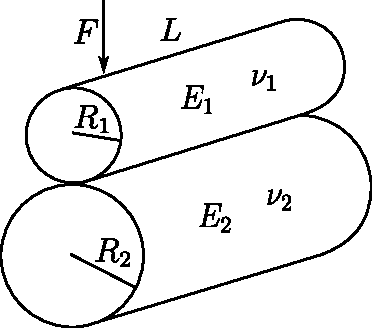
\includegraphics[width=0.7\textwidth]{images/hertzian_two_cylinders.pdf}
    \caption{Stik dveh vzporednih valjev.}
    \label{fig:hetzian-two-cylinders}
  \end{subfigure}
  \begin{subfigure}[t]{0.50\textwidth}
    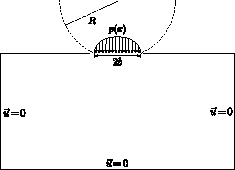
\includegraphics[width=\textwidth]{images/hertzian_analytical_setup.pdf}
    \caption{Robni pogoji za numerično rešitev.}
    \label{fig:hertz-analytical-setup}
  \end{subfigure}
  \caption{Obravnavan Hertzev kontaktni problem.}
  \label{fig:hertz-skica}
\end{figure}

Območje stika med valjema je širine $2b$, kjer je
\begin{equation}
  b = 2\sqrt{\frac{F R}{\pi E^\ast}},
\end{equation}
pri čemer je $F$ sila na enoto dolžine, $R$ kombiniran krivinski radij dan z $\frac1R = \frac1{R_2}
+ \frac1{R_2}$ in $E^\ast$ kombiniran elastični modul dan z $\frac{1}{E^\ast} = \frac{1-\nu_1^2}{E_1}
+ \frac{1-\nu_2^2}{E_2}$. Pritisk na kontaktno površino je dan z
\begin{equation}
  p(x) = \begin{cases}
    p_0 \sqrt{1-\frac{x^2}{b^2}}; & |x| < b \\
    0; & \text{sicer}
  \end{cases}, \qquad p_0 = \sqrt{\frac{FE^\ast}{\pi R}}.
\end{equation}
Pri enem valju pošljemo krivinski radij proti
neskončno in problem prevedemo na ravninskega preko predpostavke o ravninski napetosti.

Numerično želimo izračunati pomike in napetosti v materialu, zato rešimo stacionarno Navierovo
enačbo~\eqref{eq:navier-stac}. Rešujemo problem
\begin{align}
  (\lambda + \mu) \nabla(\nabla\cdot \vu) + \mu \nabla^2 \vu &= 0 \quad \text{ na } \Omega =
  (-\infty, \infty) \times (-\infty, 0) \nonumber \\
  \vt(x, 0) &= -p(x)\vj, \label{eq:hertzian-problem}  \\
  \lim_{x, y\to\infty} \vu(x, y) &= 0. \nonumber
\end{align}
Analitične rešitve kontaktnih problemov se ponavadi izpelje iz Flamantove
rešitve~\cite[str.~294]{slaughter2012linearized}, ki v posebnem primeru reši problem
točkovnega pritiska na polravnino za robni pogoj $\vt(x, 0) = p_0\delta(x)\vj$. Druge rešitve lahko
dobimo s konvolucijo s Flamantovo rešitvijo ali pa z metodo kompleksnih potencialov, kot je to
narejeno v~\cite{mcewen1949stresses} še za nekoliko splošnejši problem. Od tam dobimo tudi
analitično rešitev v zaprti obliki za napetost, ki se izraža v splošni točki $(x, y)$ s funkcijama
$m$ in $n$,
\begin{align}
  m^2 &= \frac{1}{2} \left(\sqrt{\left(b^2-x^2+y^2\right)^2+4 x^2 y^2}+b^2-x^2+y^2\right), \\
  n^2 &= \frac{1}{2} \left(\sqrt{\left(b^2-x^2+y^2\right)^2+4 x^2 y^2}-(b^2-x^2+y^2)\right),
\end{align}
kjer je $m=\sqrt{m^2}$ in $n=\sgn(x)\sqrt{n^2}$. Z njuno pomočjo zapišemo napetosti
\begin{align}
  \sigma_{xx} &= -\frac{p_0}{b}\left[m\left(1 + \frac{y^2 + n^2}{m^2 + n^2}\right)+2y\right], \\
  \sigma_{yy} &= -\frac{p_0}{b}m\left(1 - \frac{y^2 + n^2}{m^2 + n^2}\right), \\
  \sigma_{xy} &= \sigma_{yx} = \frac{p_0}{b}n\left(\frac{m^2 - y^2}{m^2 + n^2}\right).
\end{align}

S pomočjo zgornje rešitve bomo analizirali napako numerične rešitve.
Analitične vrednosti napetosti v okolici kontakta so prikazane na sliki~\ref{fig:hertz-analytical}.

\begin{figure}[!h]
  \centering
  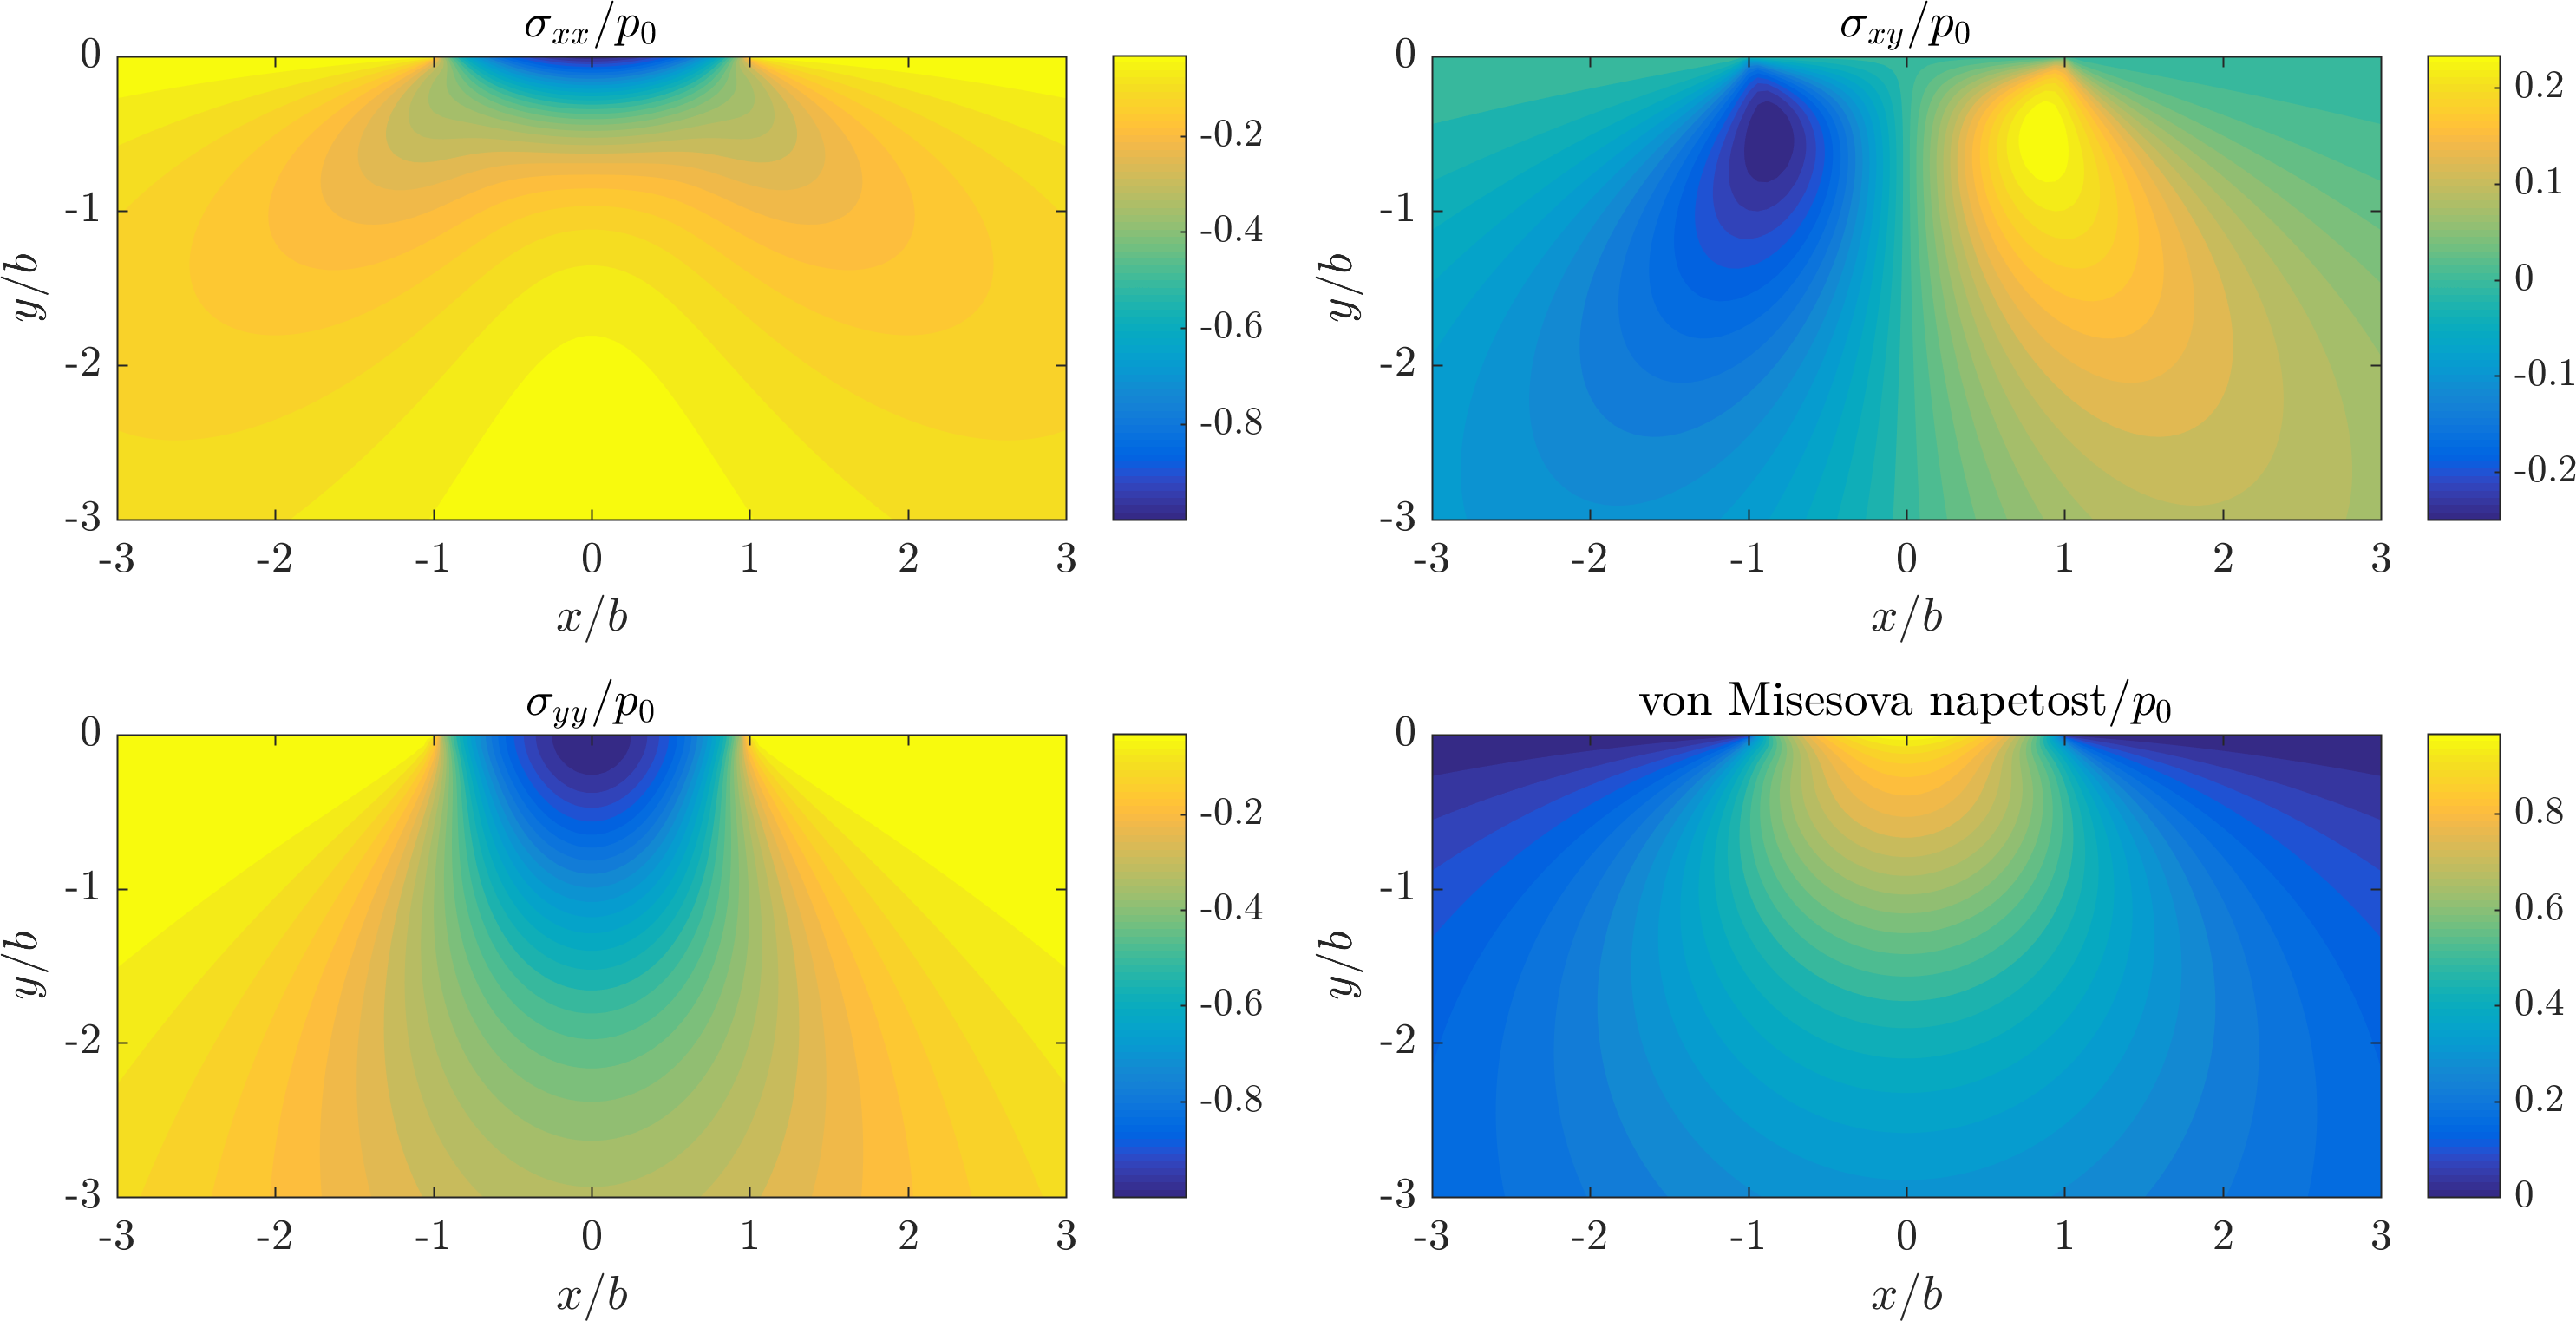
\includegraphics[width=\textwidth]{images/hertzian_analytical.png}
  \caption{Napetosti pod območjem kontakta med valjem in polravnino.}
  \label{fig:hertz-analytical}
\end{figure}

Za normo napake si zopet izberemo diskretno $L_\infty$ normo, le da tokrat
primerjamo napetosti $\sigma_{xx}, \sigma_{yy}$ in $\sigma_{xy}$. Pošteno je primerjati
brezdimenzijske količine $\sigma_{xx}/p_0$, saj so neodvisne od izbire $b$ in $p_0$.
Za napako med izračunanimi vrednostmi, označenimi s strešico, in pravimi vrednostmi, brez strešice,
tako vzamemo
\begin{equation}
  e_\infty = \max_{x\in \X} \{\max\{|\sigma_{xx}(x)-\hat{\sigma}_{xx}(x)|,
                                   |\sigma_{yy}(x)-\hat{\sigma}_{yy}(x)|,
                                   |\sigma_{xy}(x)-\hat{\sigma}_{xy}(x)| \}\} / p_0.
\end{equation}

Poskusimo problem rešiti na enak način kot pri problemu vpetega nosilca.
Za numerično reševanje neskončno domeno omejimo na $[-H, H] \times [-H, 0]$ za dovolj velik $H$
in na robu postavimo premik na 0, kot prikazano na sliki~\ref{fig:hertz-analytical-setup}. Na
zgornjem robu domene kot prej zahtevamo predpisano napetost. Za parametre problema smo vzeli $F =
\unit[543]{N/m}$, $E_1 = E_2 = \unit[72.1]{GPa}$, $\nu_1 = \nu_2 = 0.33$, $R_1 = R = \unit[1]{m}$.
Od tod dobimo širino kontakta $b = \unit[0.13]{mm}$ in maksimalni tlak $p_0 = \unit[2.6]{MPa}$.
Za $H$ izberimo \unit[10]{mm}, torej približno 75-krat večjo domeno, kot je pojav, ki ga opazujemo.

Numerično smo problem rešili na dva načina, z uporabo 9 monomov in 9 Gaussovih funkcij z $\sigma_b =
350\,r_\chi$. Obakrat smo uporabili Gaussovo utež z $\sigma = r_\chi$. Za reševanje linearnega
sistema enačb smo uporabili iterativni BiCGSTAB algoritem z ILUT predpogojevanjem. Uporabili smo
parametra $p=20$ in $\tau = 10^{-5}$. BiCGSTAB algoritem smo iterirali največ 300-krat ali dokler ni
bila ocena napake pod $10^{-13}$. Algoritem je v vseh primerih konvergiral. Na
sliki~\ref{fig:hertz-convergence} je prikazana konvergenca numerične metode.

\begin{figure}[!h]
  \centering
  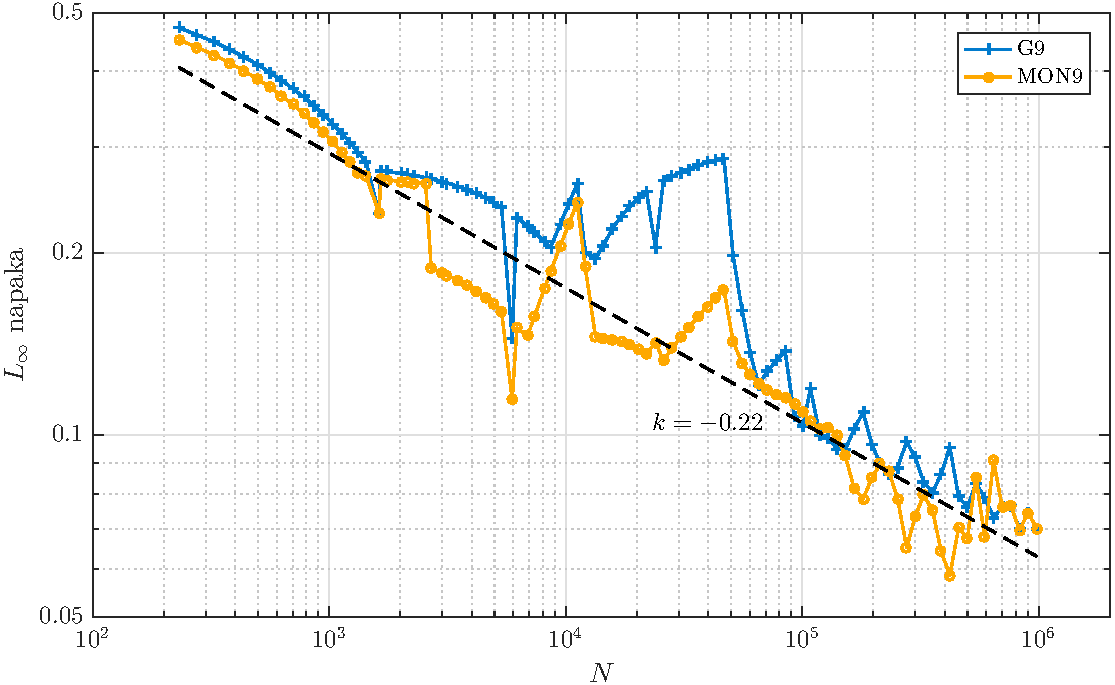
\includegraphics[width=\iw]{images/hertzian_convergence.pdf}
  \caption[Konvergenca metode pri reševanju Hertzevega kontaktnega
  problema.]{Konvergenca metode pri reševanju Hertzevega kontaktnega
  problema~\eqref{eq:hertzian-problem}.}
  \label{fig:hertz-convergence}
\end{figure}

Vidimo, da je konvergenca zelo neregularna, nizkega reda in da imamo relativno visoko napako.
Visoka napaka je posledica relativno redke diskretizacije, saj tudi pri $N = 10^6$ točkah v domeni
to pomeni, da imamo le 10 točk na dolžino $b$. Neregularnost izhaja iz neregularnosti robnih
pogojev, funkcija $p$ namreč ni niti Lipschitzeva in njen vogal pri $\pm b$ je težko dobro
aproksimirati. Celotno območje $[-2b, 2b] \times [-2b, 0]$ v bližnji okolici kontakta torej popisuje
le slabih 800 točk. Iz grafa konvergence pri problemu vpetega nosilca na
sliki~\ref{fig:cantilever-beam-convergence} odčitamo, da bi pri takem številu točk imeli napako
okoli $0.04$, kar je v enakem velikostnem razredu. Večjo napako v našem primeru gre pripisati
aproksimaciji robnih pogojev in njihovi neregularnosti. Za zmanjšanje napake imamo dve strategiji,
glede na to od kje izvira glavni del napake: ali povečamo domeno ali pa izboljšamo diskretizacijo.
Oglejmo si najprej, kaj lahko pridobimo s povečanjem domene, in kako vemo, kdaj smo izbrali dovolj
velik $H$. Na sliki~\ref{fig:hertz-domain-too-small} so prikazane napake v odvisnosti od velikosti
domene pri različnih gostotah diskretizacij.

\begin{figure}[!h]
  \centering
  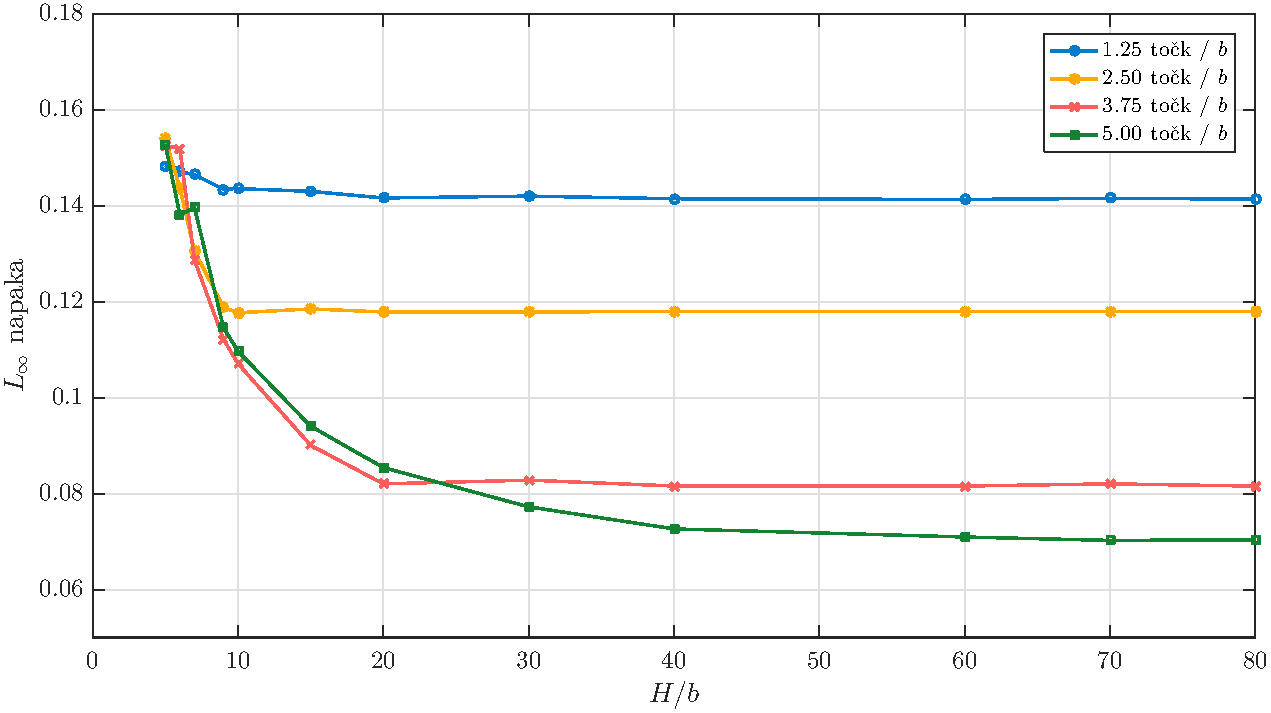
\includegraphics[width=\iw]{images/hertzian_domain_too_small2.pdf}
  \caption[Napaka v odvisnosti od velikosti domene.]{Napaka pri različnih
  gostotah diskretizacij v odvisnosti od velikosti domene.}
  \label{fig:hertz-domain-too-small}
\end{figure}

Vidimo, da na začetku napaka, povzročena z netočnimi robnimi pogoji, pada, in ko pade pod vrednost
napake, ki je nastala zaradi diskretizacije, večanje $H$ ne pomaga več. Pri bolj natančnih
diskretizacijah moramo vzeti tudi večji $H$, saj je napaka diskretizacije toliko nižja. Če torej
ugotovimo, da se konvergenca ustavi ali ne nadaljuje več z enakim redom kot prej, smo najverjetneje
zadeli ob napako zaradi končnih robnih pogojev.

Pri veliki domeni je računsko nemogoče enakomerno gosto večati diskretizacijo. Neposredna rešitev je
lokalno zgoščevanje mreže v območju, kjer pričakujemo največjo napako, in sicer v okolici kontakta.
Izberimo $H = \unit[1]{m} \approx 75\,000\, b$ in zgostimo mrežo kot opisano v
razdelku~\ref{sec:goscenje}. Za parametre zgoščevanja smo izbrali $\ell = 8$ in $f = 0.4$.
Najprej jo primarno zgostimo v pravokotnikih oblike
\begin{equation}
   [-hb, hb] \times [0, hb], \text{ za } h \in \{1000, 500, 200, 100, 50, 20, 10, 5, 4, 3, 2\},
\end{equation}
nato še sekundarno zgostimo domeno okoli točk $\pm b$ na površini v pravokotnikih oblike
\begin{equation}
  [c-hb, c+hb] \times [-hb, 0], \text{ za } c = \pm b \text{ in } h \in \{0.4, 0.3, 0.2, 0.1, 0.05, 0.0025\}.
\end{equation}
Na sliki~\ref{fig:hertz-refined-domain} je prikazan kos tako zgoščene domene, na
sliki~\ref{fig:hertz-refined-domain-density} pa gostota diskretizacije v domeni, podana kot razmerje
med razdaljo do najbližjega soseda in največjo možno razdaljo do najbližjega soseda.

\begin{figure}[h]
  \centering
  \begin{subfigure}[t]{0.45\textwidth}
    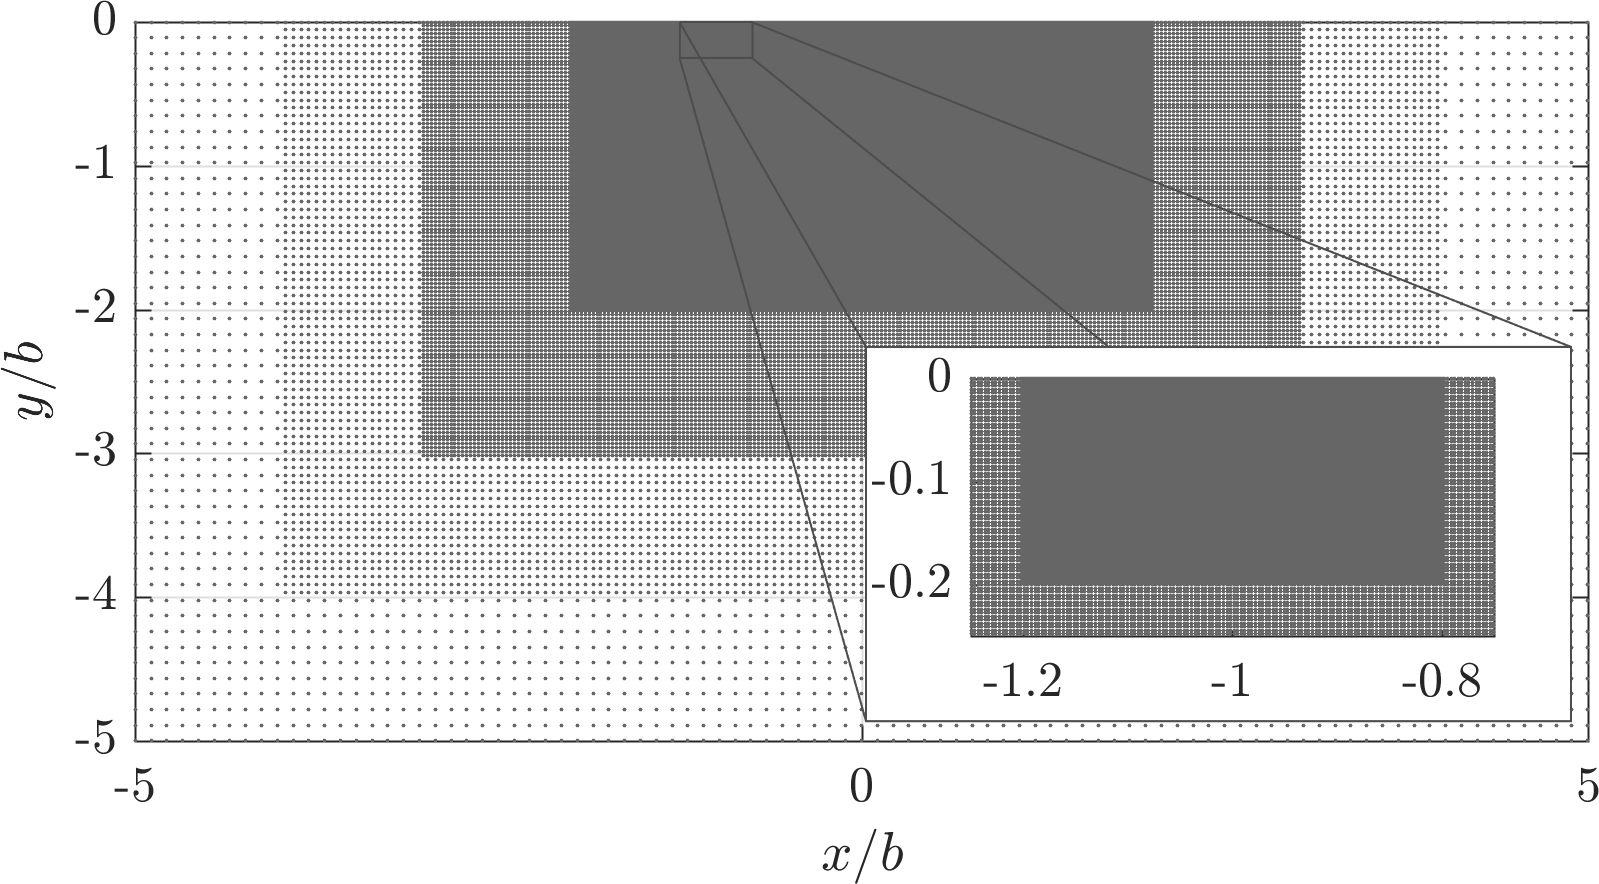
\includegraphics[width=\textwidth]{images/hertzian_refined_domain.png}
    \caption[Sedemnajstkrat zgoščena diskretizacija.]{Sedemnajstkrat zgoščena diskretizacija okoli področja zanimanja.}
    \label{fig:hertz-refined-domain}
  \end{subfigure}
  \begin{subfigure}[t]{0.45\textwidth}
    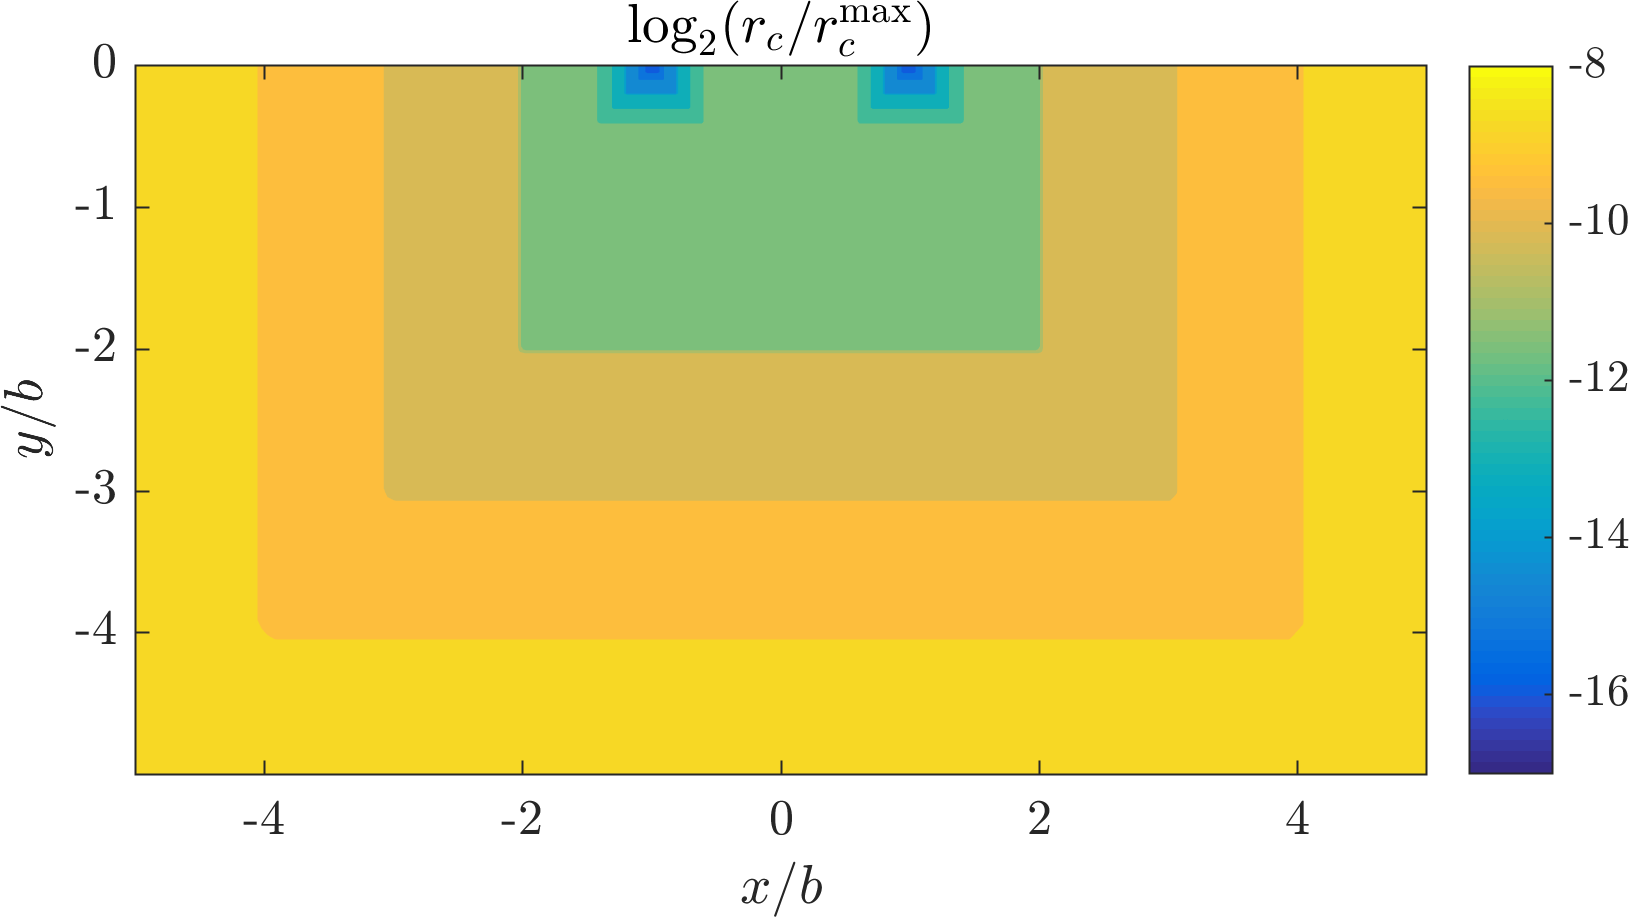
\includegraphics[width=\textwidth]{images/hertzian_refined_domain_density.png}
    \caption{Gostota diskretizacije zgoščene domene.}
    \label{fig:hertz-refined-domain-density}
  \end{subfigure}
  \caption[Primer zgoščene domene s katero rešujemo Hertzev kontaktni
  problem.]{Primer sedemnajstkrat zgoščene domene s pomočjo katere lahko
  bolj natančno rešimo Hertzev kontaktni problem~\eqref{eq:hertzian-problem}.}
  \label{fig:hertz-refined-domain-together}
\end{figure}

Rešimo problem na zgoščeni domeni z uporabo Gaussovih funkcij s parametrom oblike $\sigma_b = 350\,
r_c$, Gaussovo utežjo s $\sigma_w = r_c$ in $n = m = 9$. Sistem enačb rešimo z iterativnim
BiCGSTAB algoritmom z ILUT predpogojevanjem. Uporabimo parametra $p=100$ in $\tau = 10^{-6}$.
BiCGSTAB algoritem iteriramo največ 1000-krat ali dokler ni ocena napake pod $10^{-15}$.
Algoritem je v vseh primerih konvergiral. Na sliki~\ref{fig:hertz-refined-convergence} je prikazana
konvergenca numerične metode pri različnih nivojih sekundarnega zgoščevanja.

\begin{figure}[h]
  \centering
  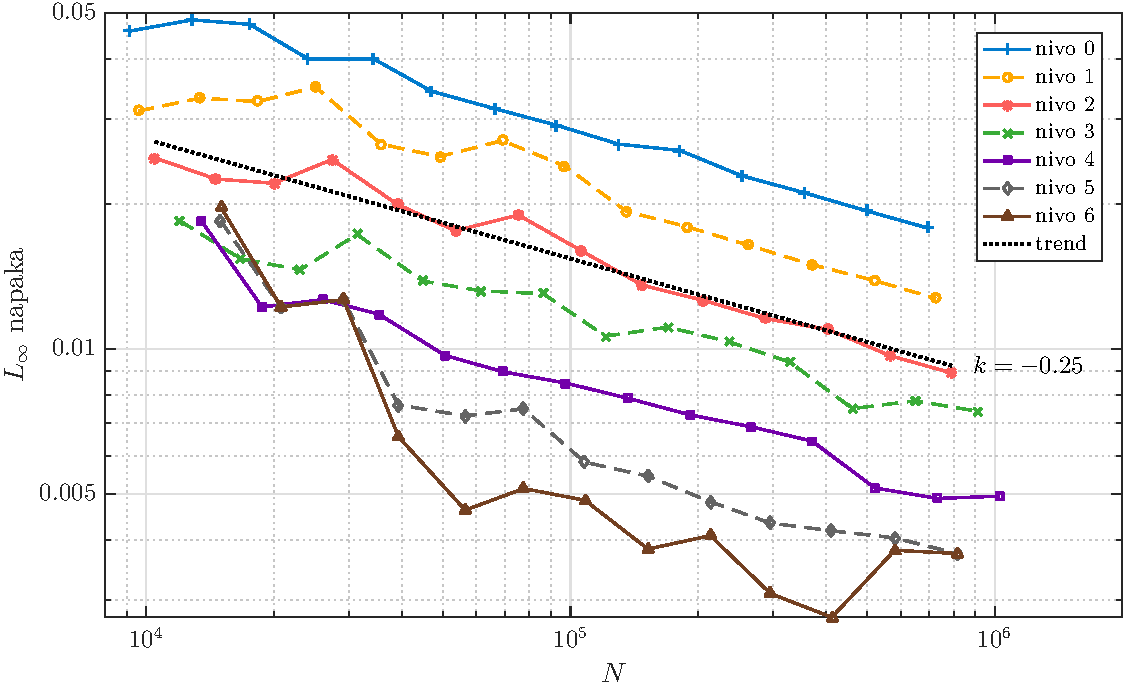
\includegraphics[width=\iw]{images/hertzian_refine_levels_convergence.pdf}
  \caption{Napaka metode pri različnih nivojih sekundarnega zgoščevanja.}
  \label{fig:hertz-refined-convergence}
\end{figure}

Vidimo, da zgoščevanje zelo pomaga. Že samo pri primarnem zgoščevanju in $N = 10^4$ je napaka manjša
kot smo jo bili sposobni doseči brez zgoščevanja. Vsak dodaten nivo zgoščevanja še izboljša
aproksimacijo. Numerična rešitev, pridobljena z najfinejšo diskretizacijo je prikazana na
sliki~\ref{fig:hertz-solution}.

\begin{figure}[!h]
  \centering
  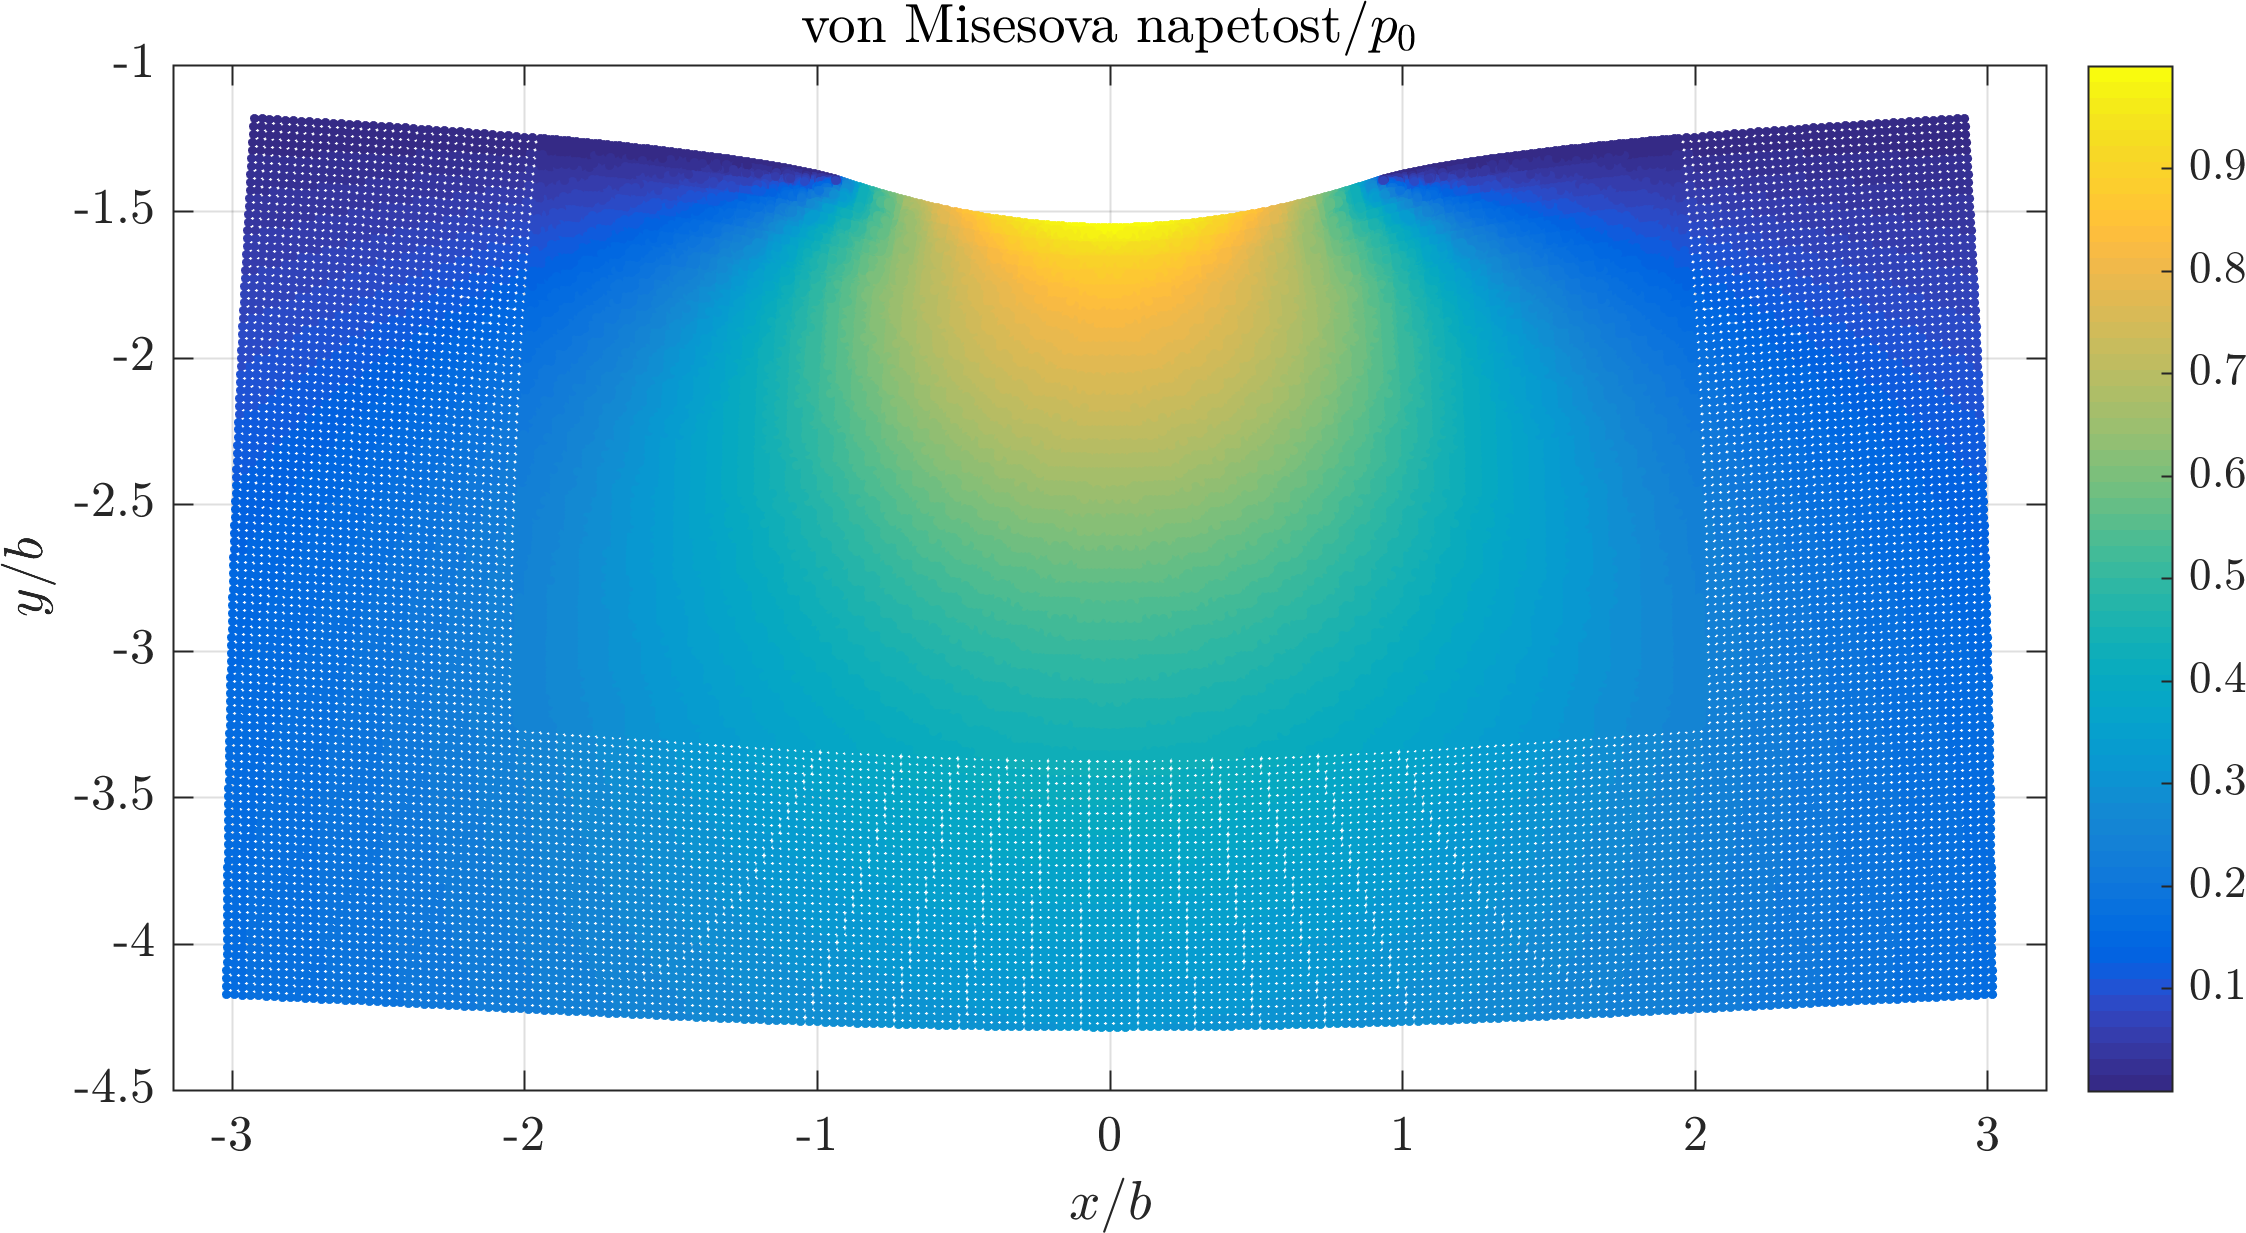
\includegraphics[width=\iw]{images/hertzian_solution_deformed_vm.png}
  \caption[Numerična rešitev Hertzevega kontaktnega problema.]{Numerična
  rešitev Hertzevega kontaktnega problema~\eqref{eq:hertzian-problem}. Zaradi
  boljše vidnosti so pomiki povečani za faktor $10^5$.}
  \label{fig:hertz-solution}
\end{figure}

\section{Zgled iz mehanike utrujenosti materialov}
\label{sec:fwo}
Oglejmo si še nekoliko bolj konkreten primer elastostatičnega problema iz področja mehanike utrujanja
materialov \ang{fretting fatigue}. Ena izmed oblik utrujanja je obraba materiala zaradi drgnjenja.
Drgnjenje je ponavadi oscilatorno gibanje z majhno amplitudo in skrajša življenjsko dobo materiala tudi
do \unit[50]{\%}~\cite{jeung2015crack} glede na življenjsko dobo, pri kateri oscilacij ne bi bilo.
To je vsekakor dovolj dober motiv, da je razumevanje tega pojava pomembna znanstvena disciplina.
Eden izmed pogostih eksperimentov za razumevanje tega pojava se izvede tako, da se ploščat kos
materiala, ki ga imenujmo \emph{vzorec}, vpne na enem koncu, medtem ko drug konec periodično
raztegujemo z napetostjo $\sax$~\cite{hojjati2014prediction}. Z drugih dveh strani na vzorec
pritiskata dve cilindrični glavi z normalno silo $F$, ki se tudi gibljeta oscilatorno tangentno na
površino materiala in nanj delujeta s tangentno silo $Q$. Shema eksperimenta je prikazana na
sliki~\ref{fig:fwo-shema}, fotografija njegove izvedbe pa na sliki~\ref{fig:fwo-experiment}.

\begin{figure}[!h]
  \begin{subfigure}[t]{0.60\textwidth}
    \centering
    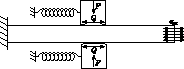
\includegraphics[width=\textwidth]{images/fwo_shema.pdf}
    \caption{Shema eksperimenta.}
    \label{fig:fwo-shema}
  \end{subfigure}
  \hspace{1em}
  \begin{subfigure}[t]{0.35\textwidth}
    \centering
    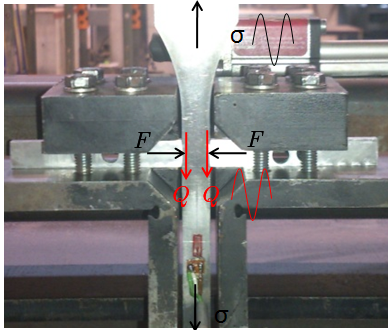
\includegraphics[width=\textwidth]{images/experiment.png}
    \caption[Fotografija eksperimenta]{Fotografija eksperimenta. \\ vir: Univerza v Luksemburgu}
    \label{fig:fwo-experiment}
  \end{subfigure}
  \caption{Eksperiment za raziskovanje utrujanja materialov.}
\end{figure}

Z eksperimentom želimo napovedati nastanek in rast razpok. Problem obravnavamo v sklopu mednarodnega
projekta (G018916N ``Multi-analysis of fretting fatigue using physical and virtual experiments'') z
Univerzo v Luksemburgu, Univerzo v Gentu in Inštitutom ``Jožef Stefan''  tudi
numerično~\cite{pereira2016convergence}. Vloga Inštituta ``Jožef Stefan'' in Univerze v Luksemburgu
je razviti originalno numerično rešitev problema, saj do sedaj uporabljena komercialna rešitev
ABAQUS\textregistered~\cite{hibbitt2001abaqus}, ki jo uporabljajo na Univerzi v Gentu, ni zagotovila
zadovoljivih rezultatov pri simulaciji širjenja razpoke. Prvi korak k simulaciji eksperimenta je
izračun napetosti na površini kontakta. Za referenčno rešitev
uporabimo~\cite{pereira2016convergence}, kjer so predstavljeni rezultati simulacije eksperimenta v
statičnem stanju maksimalne oscilacije s tangentno silo enako $Q$ in osno napetostjo enako $\sax$.
Eksperiment ima vodoravno simetrijsko os (slika~\ref{fig:fwo-shema}) zato lahko pri simulaciji
obravnavamo samo eno glavo in polovično širino ter rezultate nato prezrcalimo. Poleg tega je
debelina materiala majhna in vse sile in napetosti so v ravnini materiala, torej ustreza
predpostavki o ravninski napetosti in ga lahko prevedemo na dve dimenziji. Problem nas spominja na
teorijo Hertzevega kontakta (\ref{sec:hertz}), le da ima prisotno tudi tangentno silo, osno napetost
in končne dimenzije. V~\cite[razdelek 2]{pereira2016convergence} so opisani analitični izrazi za
modeliranje napetosti, s katerimi cilindrična glava pritiska na vzorec. Označimo krivinski radij
glave z $R$, širino vzorca z $W$, dolžino z $L$ in debelino z $t$. Izraz za širino kontakta je enak
kot pri Hertzevem problemu, pri čemer upoštevamo, da je dolžinska gostota sile enaka $F/t$. Širina
polovice kontaktnega območja se tako izraža~z
\begin{equation}
   a = 2\sqrt{\frac{FR}{t \pi E^\ast}},
\end{equation}
normalni pritisk na kontaktno površino pa je dan z
\begin{equation}
  p(x) = \begin{cases}
    p_0 \sqrt{1-\frac{x^2}{a^2}}; & |x| < a \\
    0; & \text{sicer}
  \end{cases}, \qquad p_0 = \sqrt{\frac{FE^\ast}{t \pi R}}.
\end{equation}
Pri tem je $E^\ast$ definiran enako kot pri Hertzevem kontaktu v razdelku~\ref{sec:hertz}.
Na tangentno silo bo imel vpliv tudi koeficient trenja med površinama, ki ga, nekoliko nesrečno,
označimo z $\mu$, tako kot Lam\'ejev drugi parameter. Iz konteksta, vrednosti in dimenzij $\mu$ bo
razvidno, katero izmed količin predstavlja. Za tangentno silo predpostavimo, da je manjša kot mejna
sila trenja, ki je dana s Coulombovim zakonom kot $\mu F$. V tem primeru se kontakt razdeli na dve
območji, območje drsenja in območje lepljenja, in tangentna napetost je dana s
\begin{equation}
  \tilde q(x) = \begin{cases}
      -\mu p_0 \left(\sqrt{1 - \frac{x^2}{a^2}} - \frac{c}{a}\sqrt{1 - \frac{x^2}{c^2}}\right);& |x|
      < c \\
      -\mu p_0 \sqrt{1 - \frac{x^2}{a^2}}; & c \leq |x| \leq a \\
      0; & \text{sicer,}
    \end{cases}
\end{equation}
pri čemer je $c = a\sqrt{1 - \frac{Q}{\mu F}}$ in $\{x; |x| < c\}$ območje lepljenja.
Zgornji izraz se da prilagoditi tudi tako, da je pravilen ob prisotnosti osne napetosti
$\sax$ z uvedbo ekscentričnosti $e = \sgn(Q)\frac{a \sax}{4 \mu p_0}$.
Z njeno pomočjo izrazimo $q$ s
\begin{equation}
q(x) = \begin{cases}
-\mu p_0 \left(\sqrt{1 - \frac{x^2}{a^2}} - \frac{c}{a}\sqrt{1 - \frac{(x-e)^2}{c^2}}\right); &
|x-e| < c \\
-\mu p_0 \sqrt{1 - \frac{x^2}{a^2}}; & c \leq | x - e | \text{ in } |x| \leq a \\
0; & \text{sicer,}
\end{cases}
\end{equation}
pri čemer mora veljati $\sax \leq 4\left( 1 - \sqrt{1-\frac{Q}{\mu F}} \right)$, da ekscentričnost
ne povzroči, da bi območje lepljivosti segalo izven območja kontakta. Sedaj imamo vse pripravljeno
za numerično reševanje. Rešujemo torej problem
\begin{align}
  (\lambda + \mu) \nabla(\nabla\cdot \vu) + \mu \nabla^2 \vu &= 0, && \text{ na } \Omega =
  [-\frac{L}{2}, \frac{L}{2}]\times[-\frac{W}{2}, 0] \nonumber  \\
  \vt(x, 0) &= q(x)\vi - p(x)\vj, && \text{(napetost na vrhu)} \nonumber \\
    \vu(-\frac{L}{2}, y) &= 0,  && \text{(vpet levo)} \label{eq:fwo-problem}\\
    \vt(\frac{L}{2}, y) &= 0, \nonumber  && \text{(prost desno)}\\
    \vu(x, -\frac{W}{2})\cdot \vj &= 0, \dpar{\vu(x, -t/2)\cdot \vi}{y} = 0, \nonumber  && \text{(simetrija
    spodaj)}
\end{align}
grafično prikazan na sliki~\ref{fig:fwo-bc}.

\begin{figure}[!h]
  \centering
  \begin{subfigure}[t]{0.45\textwidth}
    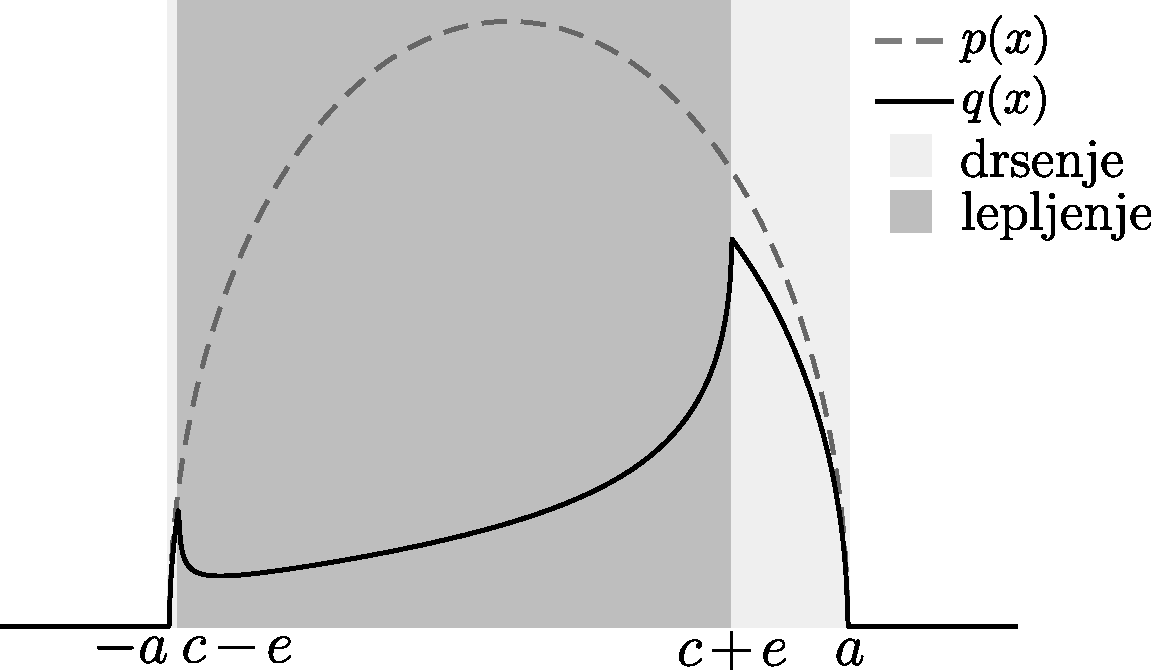
\includegraphics[width=\textwidth]{images/fwo_sample_pq.pdf}
    \caption[Primer napetosti $p(x)$ in $q(x)$.]{Primer napetosti $p(x)$ in $q(x)$ z označenima območjema drsenja in lepljenja za $R =
    \unit[50]{mm}$ in $\mu = 0.85$.}
    \label{fig:fwo-pq-example}
  \end{subfigure}
  \hspace{10pt}
  \begin{subfigure}[t]{0.45\textwidth}
    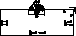
\includegraphics[width=\textwidth]{images/fwo_bc.pdf}
    \caption[Domena in robni pogoji.]{Domena in robni pogoji. Označili smo $\vu = (u, v)$, $\vt = (t_x, t_y)$.}
    \label{fig:fwo-bc}
  \end{subfigure}
  \caption{Domena in robni pogoji za numerično reševanje problema~\eqref{eq:fwo-problem}.}
  \label{fig:fwo-setup}
\end{figure}

V eksperimentu, opisanem v~\cite{hojjati2014prediction}, je bil uporabljen aluminij 2420-T3, katerega
materialni lastnosti sta  $E = \unit[72.1]{GPa}$ in $\nu = 0.33$. Vzorec je bil velikosti $t =
\unit[4]{mm}$, $W = \unit[10]{mm}$ in $L = \unit[40]{mm}$. Največji izmerjeni sili sta bili $F =
\unit[543]{N}$ v smeri $-\vj$ in $Q = \unit[155]{N}$ v smeri $-\vi$, osna napetost pa je bila $\sax
= \unit[100]{MPa}$. Numerična simulacija v~\cite{pereira2016convergence} je bila narejena za $R =
\unit[10]{mm}$ in $R = \unit[50]{mm}$ in tri različne koeficiente trenja $\mu = 0.3$, $\mu = 0.85$
in $\mu = 2$, zato tudi mi izberimo te parametre. Na Hertzevem kontaktnem
problemu~\eqref{eq:hertzian-problem} smo se naučili, kako dobro diskretizirati domeno. Tudi tukaj
uporabimo enake parametre, le goščenje domene prilagodimo manjšim dimenzijam. Metoda je za vse
izbire parametrov $R$ in $\mu$ s povečevanjem $N$ konvergirala proti limitni rešitvi. Na
sliki~\ref{fig:fwo-ujemanje} je prikazano ujemanje naše numerične rešitve z rešitvijo, izračunano
v~\cite{pereira2016convergence}, za $N = 52659$ pri manjšem in $N = 178897$ pri večjem radiju.

\begin{figure}[h]
  \centering
  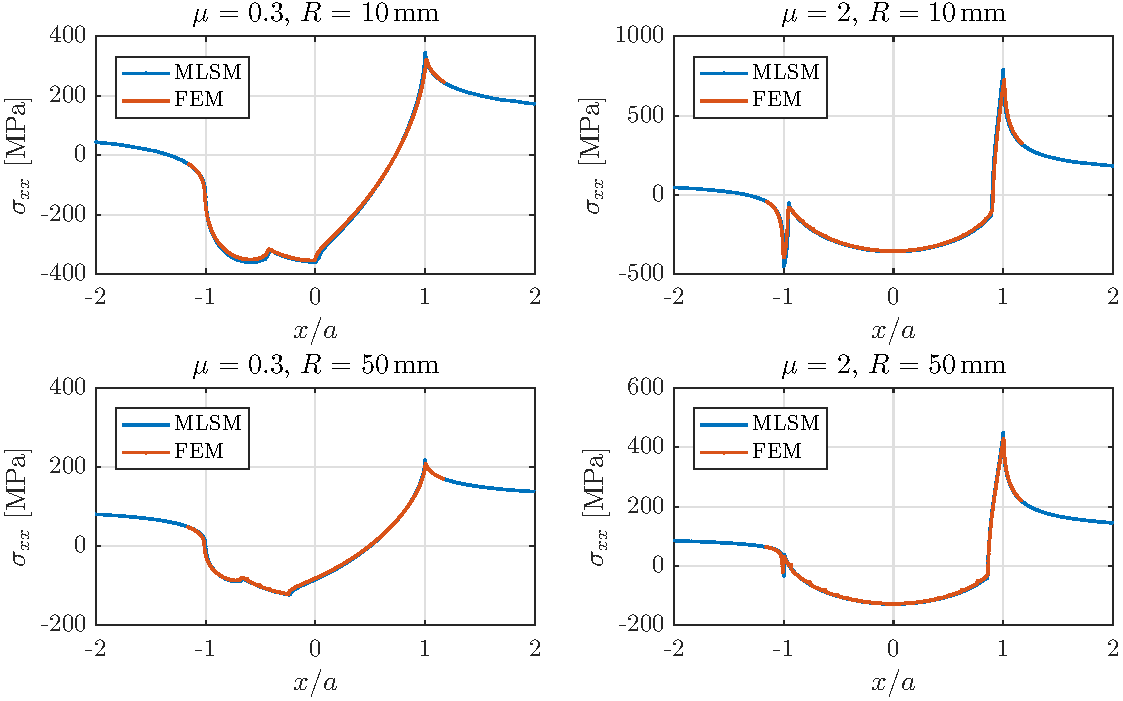
\includegraphics[width=\textwidth]{images/fwo_cases.pdf}
  \caption{Ujemanje MLSM in FEM rešitve pri analizi kontakta.}
  \label{fig:fwo-ujemanje}
\end{figure}

Vidimo, da se rešitvi dobro ujemata, a ne povsem, kar je tudi pričakovati, saj je FEM rešitev
nastala s simulacijo kontakta, MLSM pa z analitičnimi robnimi pogoji. Ujemanje rešitev kljub temu
nakazuje, da je metoda MLSM primerna tudi za reševanje problemov iz kontaktne mehanike.

Posebno zanimanje pa ima vrednost $\ts_{xx}$ v špici na desni strani kontaktne površine,
saj so raziskave pokazale, da se glavna razpoka, ki pripomore k zlomu materiala, zgodi v neposredni
bližini $x = a$. Analitična aproksimacija za največjo vrednost $\ts_{xx}$ se izraža
kot~\cite[enačba (7), str.\ 6]{pereira2016convergence}
\begin{equation}
  \ts_{xx, \max} = 2 p_0 \sqrt{\frac{\mu Q}{F}} + \sax.
\end{equation}
V tabeli~\ref{tab:sxxmax} je prikazana izračunana vrednost $\ts_{xx, \max}$ za FEM in MLSM
pri različnih $N$. Tabela vrednosti za FEM je vzeta iz~\cite[tabela 3]{pereira2016convergence}.
\begin{table}[h]
  \centering
  \begin{tabular}{ccllll} \hline
    \multicolumn{1}{c}{$\mu$} & minimalna        & \multicolumn{2}{c}{$R=\unit[10]{mm}$}              & \multicolumn{2}{c}{$R=\unit[50]{mm}$}              \\ \cline{3-6}
    & razdalja $[\unit{\mu m}]$ & \multicolumn{1}{c}{MSLM} & \multicolumn{1}{c}{FEM} & \multicolumn{1}{c}{MLSM} & \multicolumn{1}{c}{FEM} \\ \hline \hline
                              & 10                 & 325.36                   & 242.57                  & 210.78                   & 182.87                  \\
                              & 5                  & 340.99                   & 268.70                  & 216.54                   & 192.96                  \\
                              & 2.5                & 354.46                   & 290.50                  & 214.69                   & 200.09                  \\
    0.3                       & 1.25               & 350.33                   & 307.81                  & 217.82                   & 205.33                  \\
                              & 0.625              & 357.84                   & 320.33                  & 216.76                   & 208.99                  \\
                              & 0.3125             & 355.65                   & 329.94                  & 218.35                   & 212.00                  \\ \cline{2-6}
                              & analitična         & 342.28                   & 342.28                  & 208.35                   & 208.35                  \\ \hline
                              & 10                 & 479.12                   & 349.91                  & 293.75                   & 254.12                  \\
                              & 5                  & 496.08                   & 398.69                  & 305.06                   & 274.64                  \\
                              & 2.5                & 522.88                   & 440.60                  & 307.62                   & 287.93                  \\
    0.85                      & 1.25               & 527.76                   & 474.40                  & 311.77                   & 297.38                  \\
                              & 0.625              & 539.26                   & 496.58                  & 314.20                   & 303.26                  \\
                              & 0.3125             & 543.71                   & 513.08                  & 315.77                   & 308.06                  \\ \cline{2-6}
                              & analitična         & 507.82                   & 507.82                  & 283.90                   & 283.90                  \\ \hline
                              & 10                 & 686.07                   & 441.20                  & 417.73                   & 336.52                  \\
                              & 5                  & 729.38                   & 537.49                  & 435.49                   & 373.08                  \\
                              & 2.5                & 769.58                   & 612.33                  & 438.91                   & 399.72                  \\
    2.0                       & 1.25               & 785.98                   & 683.24                  & 448.12                   & 417.17                  \\
                              & 0.625              & 808.62                   & 719.75                  & 447.74                   & 428.46                  \\
                              & 0.3125             & 809.06                   & 750.50                  & 451.95                   & 436.21                  \\ \cline{2-6}
                              & analitična         & 725.56                   & 725.56                  & 382.10                   & 382.10                  \\ \hline
  \end{tabular}
  \caption{Tabela vrednosti $\ts_{xx, \max}\ [\unit{MPa}]$ za FEM, MLSM in analitično aproksimacijo pri različnih gostotah diskretizacije.}
  \label{tab:sxxmax}
\end{table}
Vidimo, da vrednosti konvergirajo k neki limiti, ki pa se razlikuje pri obeh metodah, vendar je v
istem velikostnem razredu. Naša rešitev dosega višje vrednosti $\ts_{xx, \max}$, kot je tudi
razvidno iz grafa na sliki~\ref{fig:fwo-ujemanje}. To je zato, ker rešujemo problem z danimi
analitičnimi robnimi pogoji, medtem ko FEM rešitev kontakt simulira in slabše aproksimira ostre
vogale. Primer izračunane napetosti za problem~\eqref{eq:fwo-problem} za $\mu=0.85$ in $R =
\unit[50]{mm}$ z $N = 178897$ točkami je prikazan na sliki~\ref{fig:fwo-solution}.

\begin{figure}[h]
  \centering
  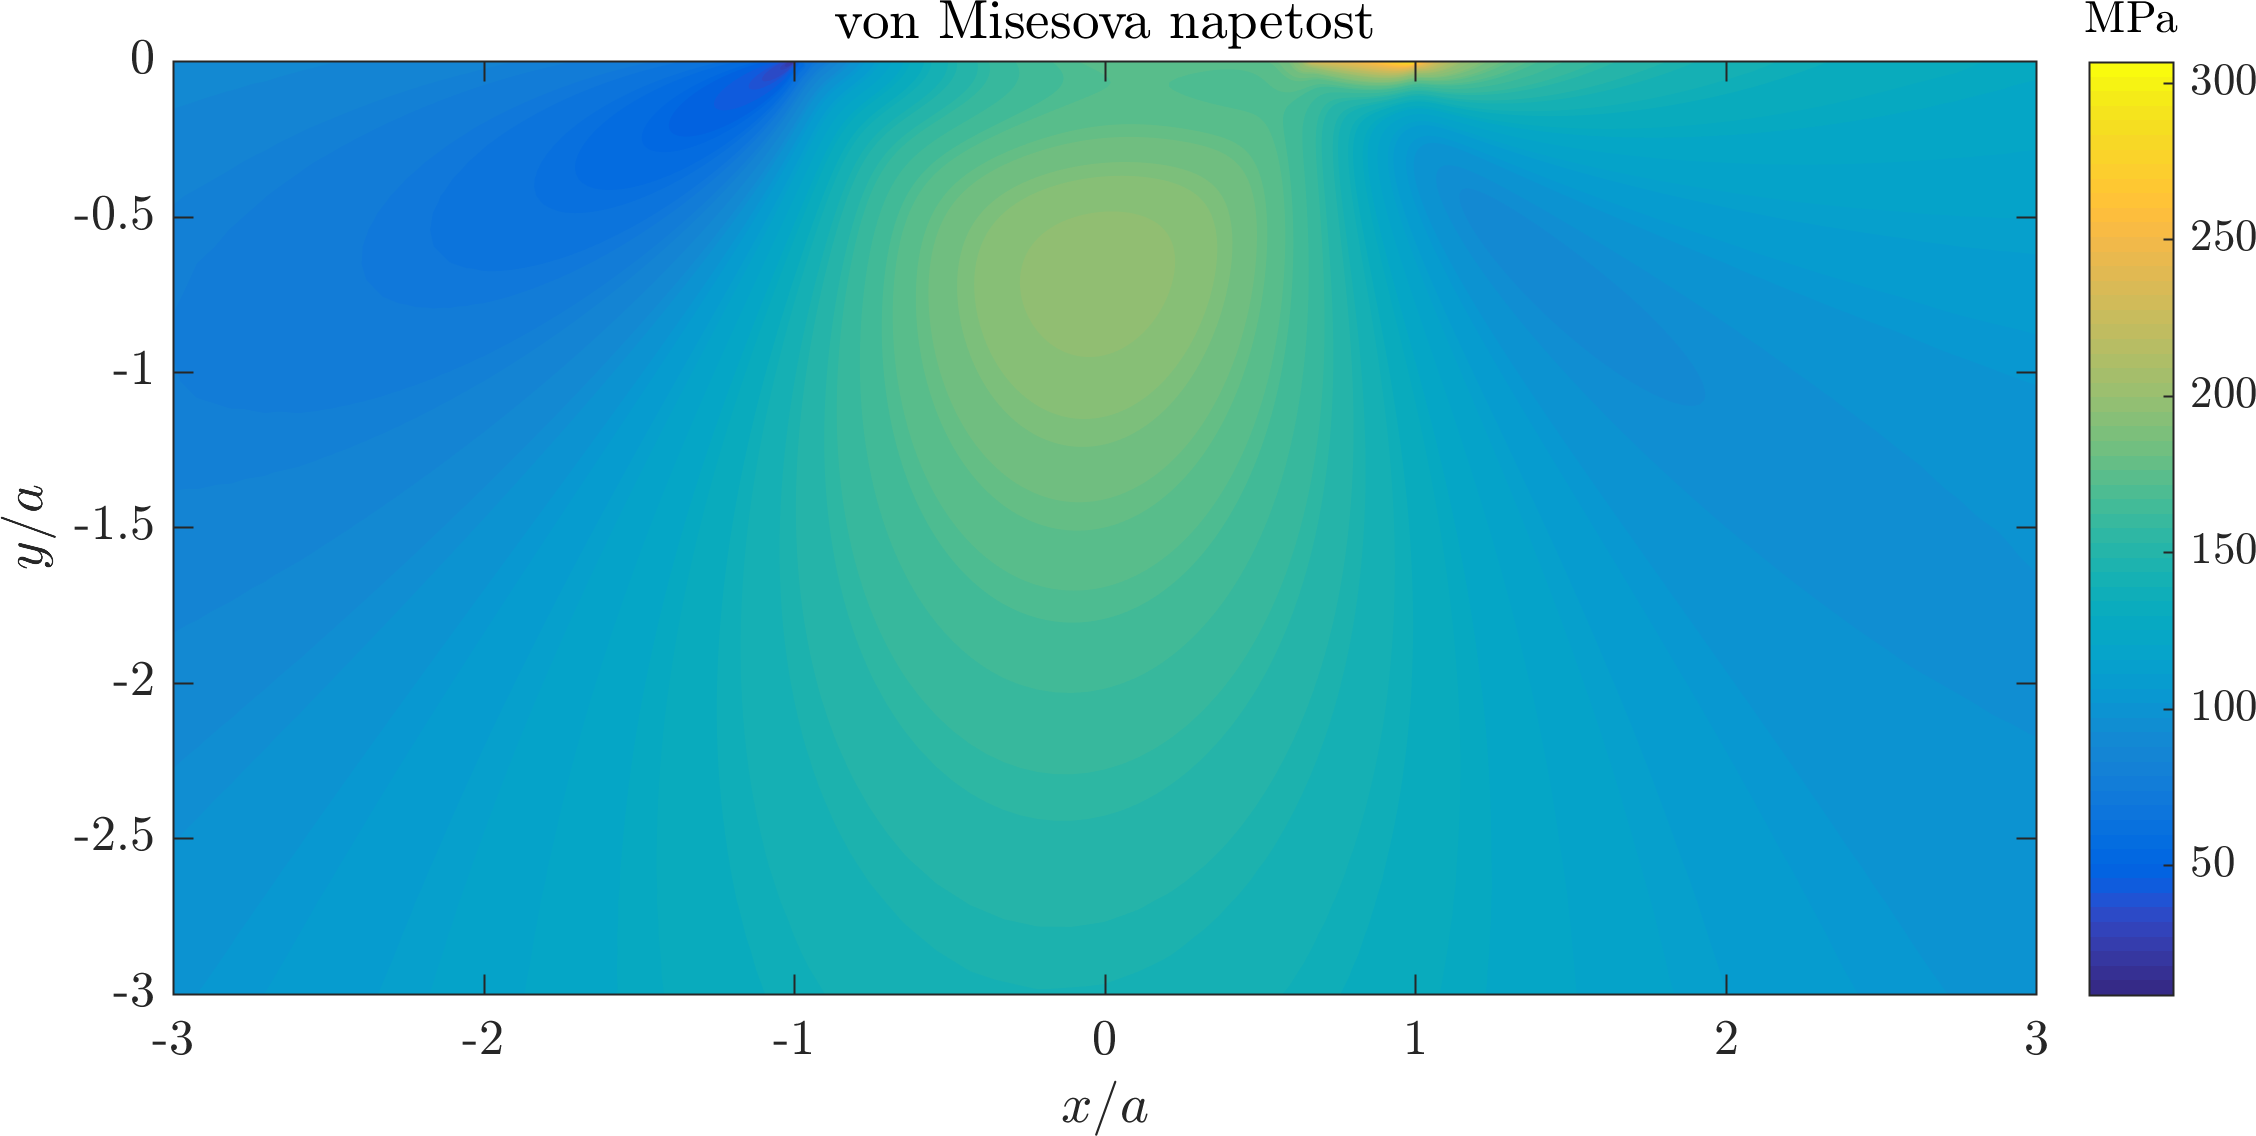
\includegraphics[width=\iw]{images/fwo_solution.png}
  \caption{Primer rešitve problema~\eqref{eq:fwo-problem} za $\mu=0.65$ in $R = \unit[50]{mm}$.}
  \label{fig:fwo-solution}
\end{figure}

Če to sliko primerjamo s sliko~\ref{fig:hertz-solution}, na kateri je rešitev Hertzevega kontaktnega
problema, opazimo podobno splošno obliko nivojnic napetosti v notranjosti, na površini pa se na
sliki~\ref{fig:fwo-solution} močno pozna vpliv tangente sile $Q$. Ta povzroči zamik nivojnic in
koncentracijo napetosti okoli točke $x = a$ na površini, ki je mnogo večja kot drugje v vzorcu.

\section{Implementacija}
\label{sec:implementacija}
Numerična metoda skupaj z vsemi dodatnimi orodji, za katere ni navedeno drugače, je bila
implementirana na oddelku E6 Instituta ``Jožef Stefan'' v Laboratoriju za vzporedno in porazdeljeno
računanje.\footnote{\url{http://www-e6.ijs.si/ParallelAndDistributedSystems/}} Implementirana je
bila v programskem jeziku \CC~\cite{stroustrup1995c++} zaradi hitrosti in dovolj močnih jezikovnih
konstruktov, kot so recimo predloge \ang{templates}, ki omogočajo elegantno implementacijo. Podoben
koncept uporablja knjižnica Eigen~\cite{eigenweb}, uporabljena za numerično linearno algebro. Za
iskanje najbližjih sosedov je bila uporabljena knjižnica ANN~\cite{mount1998ann}. Celotna
implementacija je prosto dostopna na repozitoriju programske skupine~\cite{utils_web} z
dokumentacijo, prav tako na voljo na
spletu\footnote{\url{http://www-e6.ijs.si/ParallelAndDistributedSystems/MeshlessMachine/}}.

Dejanska implementacija v grobem sledi postopku, opisanem v algoritmu~\ref{alg:metoda}. Na
sliki~\ref{fig:implementacija} je prikazan diagram izvedbe izračuna.

\begin{figure}[!h]
  \centering
  \vspace{-2ex}
  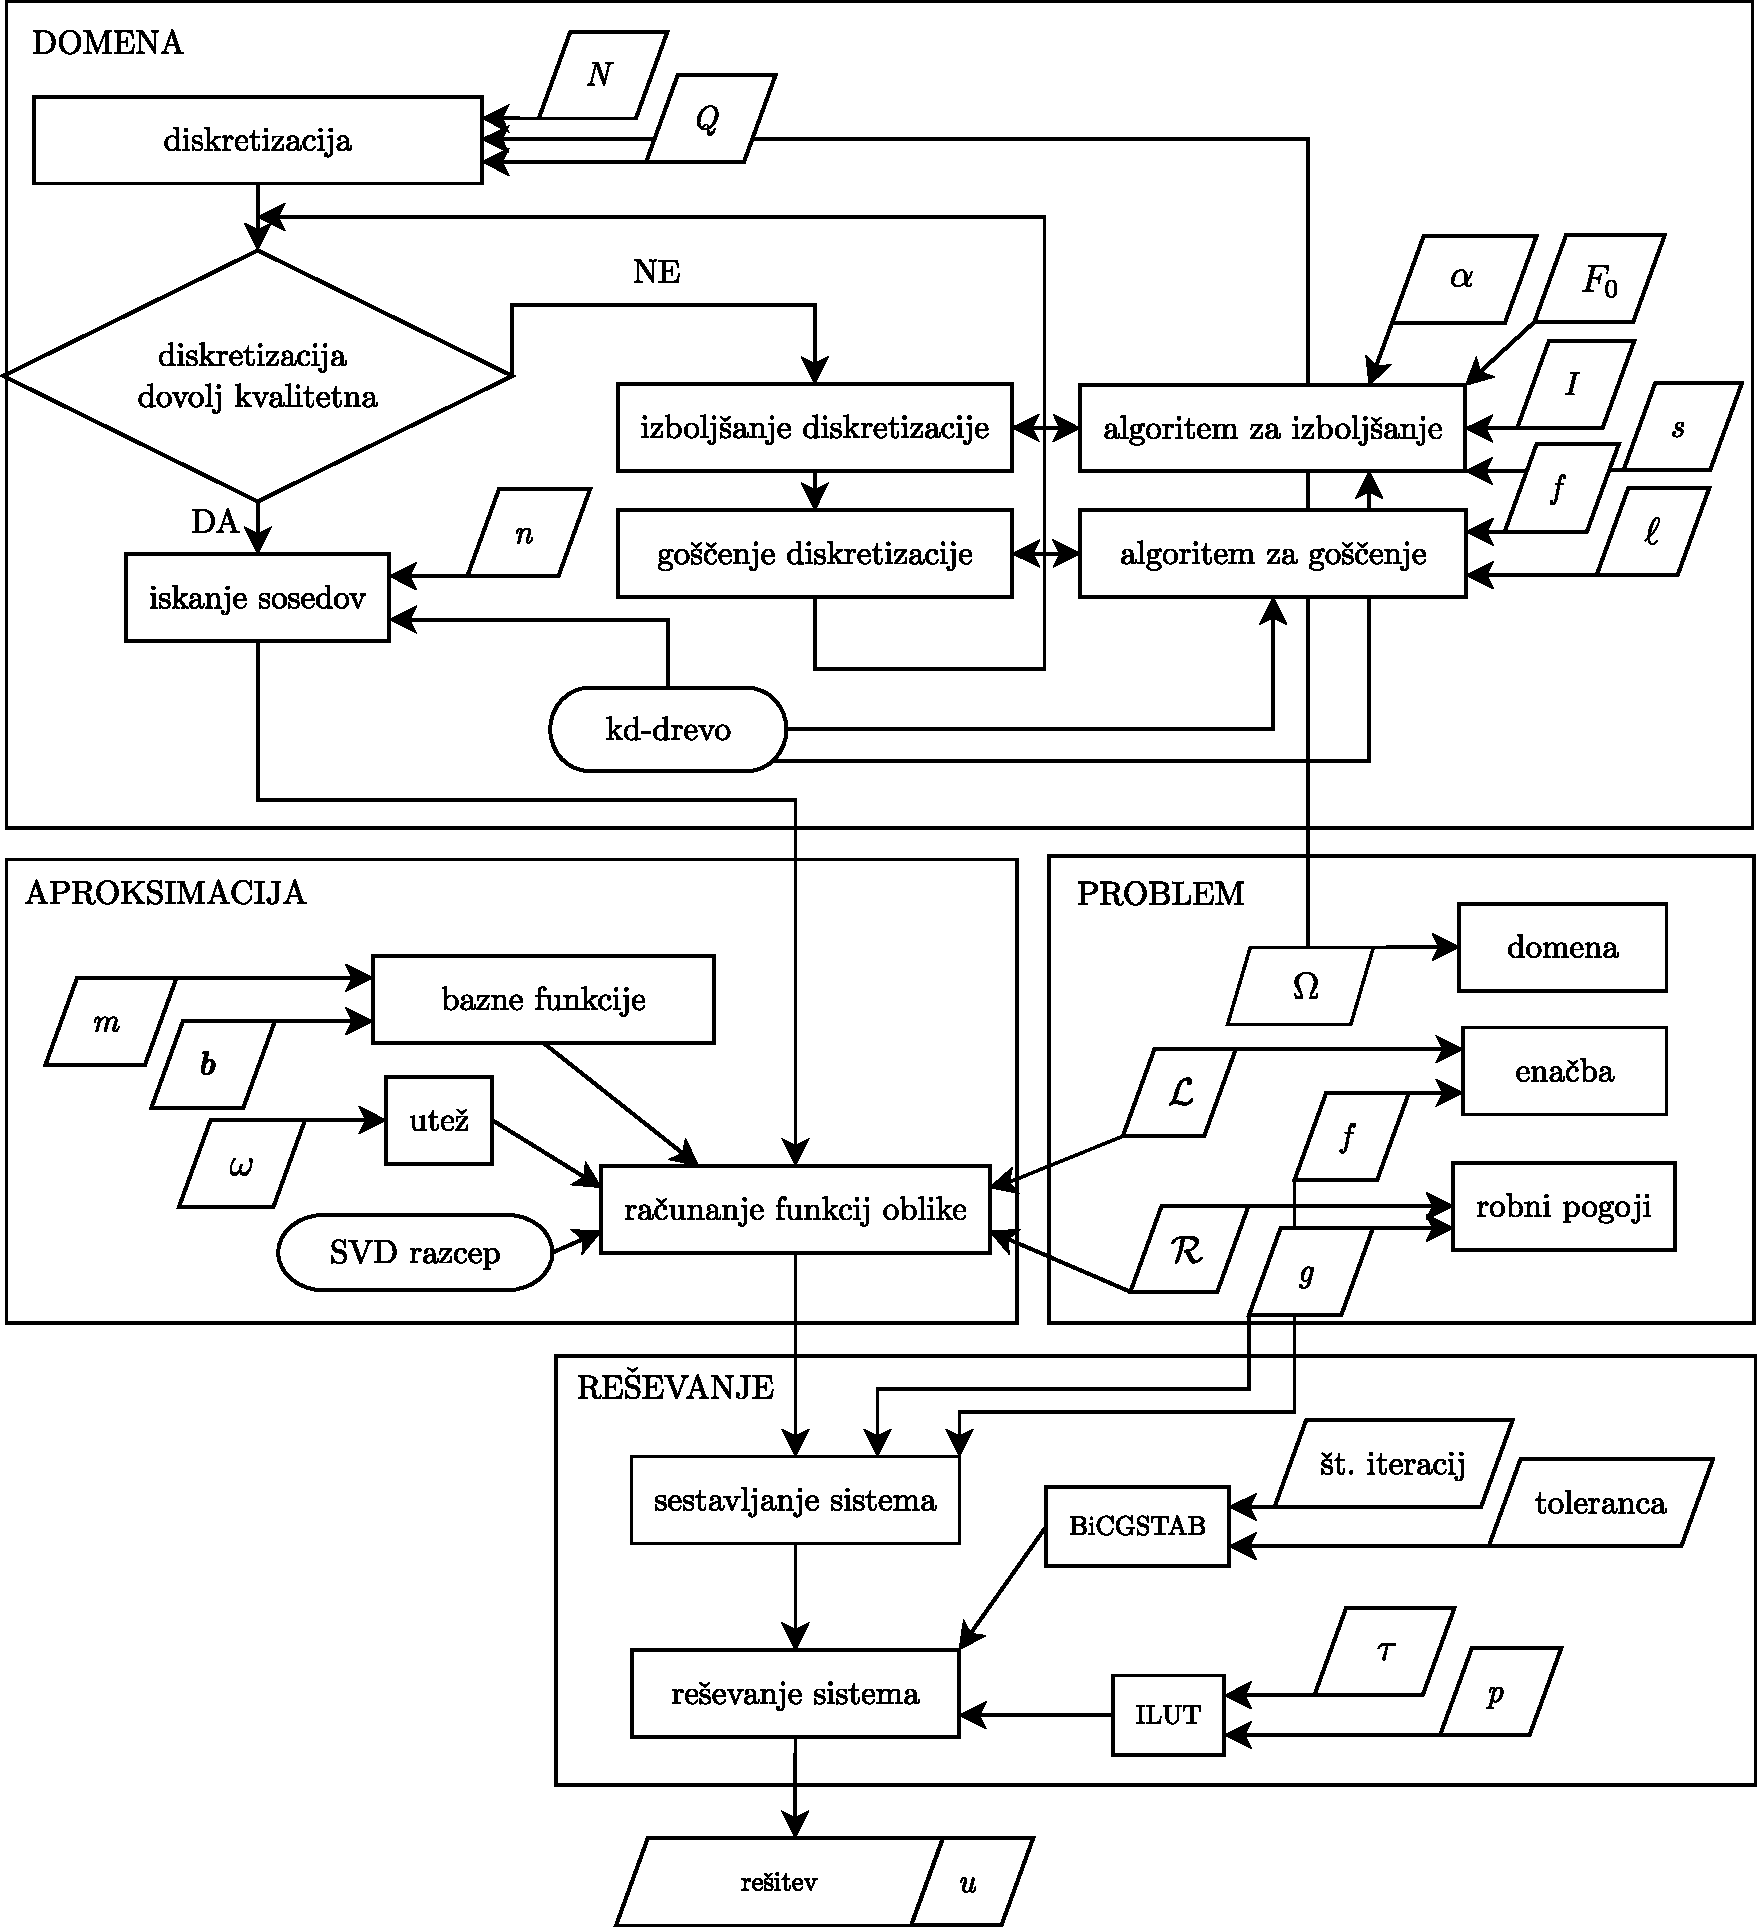
\includegraphics[width=0.95\textwidth]{images/diagram_finished.pdf}
  \vspace{-1ex}
  \caption[Diagram implementacije in izvedbe MLSM]{Diagram implementacije in
  izvedbe algoritma~\ref{alg:metoda}.}
  \label{fig:implementacija}
  \vspace{-5ex}
\end{figure}

\subsection{Vzporedno računanje}
Oglejmo si še možnost pospešitve računanja s pomočjo paralelizacije.
Vse meritve časa v tem razdelku so bile narejene na računalniku z dvema centralno procesnima enotama
\texttt{Intel(R) Xeon(R) CPU E5-2620 v3 @ 2.40GHz} s po 6 jedri, od katerih vsako jedro podpira dve
niti izvajanja, in \unit[64]{GiB} pomnilnika. Programi so bili prevedeni z Intelovim~\CC{}
prevajalnikom \texttt{icpc}  s stikali \texttt{-std=c++11 -O3 -DNDEBUG}
na operacijskem sistemu Ubuntu Linux 14.04. Za matematične operacije je bila uporabljena Intelova
knjižnica MKL~\cite{mkl}. Pri paralelizaciji je bila uporabljena Intelova implementacija knjižnice
OpenMP~\cite{dagum1998openmp} za paralelizacijo z deljenim pomnilnikom. Za reševanje sistemov
linearnih enačb je bila uporabljena Intelova implementacija sistema Pardiso~\cite{pardiso}. Vse
knjižnice in programi so verzije 2016.1.150 za Linux.

Oglejmo si najprej, kateri deli postopka so časovno najbolj potratni. Iz časovne analize v
razdelku~\ref{sec:casovna-zahtevnost} lahko sklepamo, da je to računanje funkcij oblike,
ki traja $O(m^2n N)$ časa ali pa reševanje sistema. Da bi bolje razumeli, koliko časa stane kateri
del, to izmerimo. Na sliki~\ref{fig:poisson-square-time-distribution} vidimo porazdelitev časa, ki ga posamezni
kosi metode potrebujejo pri reševanju Poissonovega robnega problema~\eqref{eq:poisson-problem}.

\begin{figure}[!h]
  \centering
  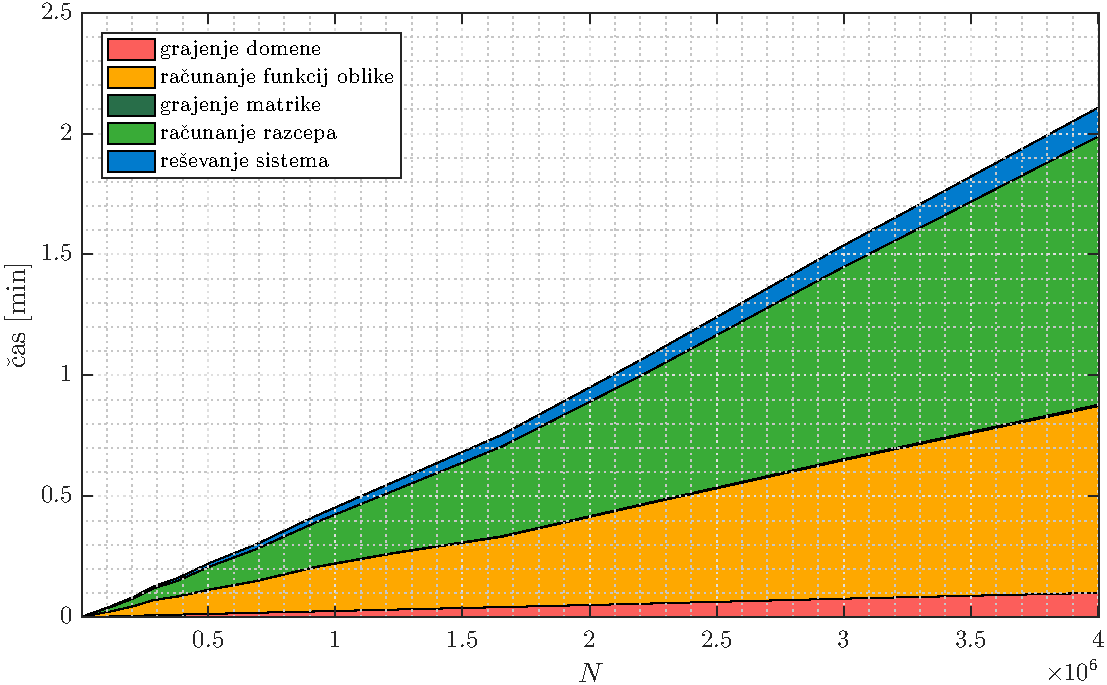
\includegraphics[width=\iw]{images/poisson_square_time_distribution_1.pdf}
  \caption[Čas izvajanja delov programa pri reševanju Poissonove enačbe.]{Čas
  izvajanja posameznih delov programa pri reševanju
  problema~\eqref{eq:poisson-problem}.}
  \label{fig:poisson-square-time-distribution}
\end{figure}

Vidimo, da sta najdražja dela res računanje funkcij oblike in reševanje sistema, zato se ju najbolj
splača paralelizirati. Zanko, ki računa funkcije oblik na vrstici~\ref{line:shape-loop}
algoritma~\ref{alg:metoda} lahko trivialno paraleliziramo, saj so operacije neodvisne med seboj,
deljeni podatki pa se ne spreminjajo. Paralelizacija reševanja razpršenega sistema linearnih enačb
ni tako enostavna in je področje mnogo raziskav z veliko razvitimi sistemi za reševanje, kot na
primer Pardiso~\cite{pardiso}, PaStiX~\cite{henon2002pastix} in MUMPS~\cite{amestoy2000mumps}.
Zaradi najlažje integracije z Eigen in dostopnosti v MKL knjižnici za osnovni test izberemo
Pardiso~\cite{pardiso}. Isti robni problem sedaj rešimo vzporedno s $k$ nitmi in s $t_k(N)$ označimo
čas izvajanja programa s $k$ nitmi na problemu z $N$ točkami v domeni. Opazovali bomo \emph{faktor
pohitritve} \ang{speed-up}
\begin{equation}
   f_k(N) = t_k(N) / t_1(N).
\end{equation}
Vrednost $f_3(10^6) = 2.5$ pove, da problem velikosti $10^6$ rešimo 2.5-krat hitreje s tremi
nitmi izvajanja kot z eno samo. Graf faktorjev pohitritve je prikazan na
sliki~\ref{fig:poisson-square-speedup}.

\begin{figure}[!h]
  \centering
  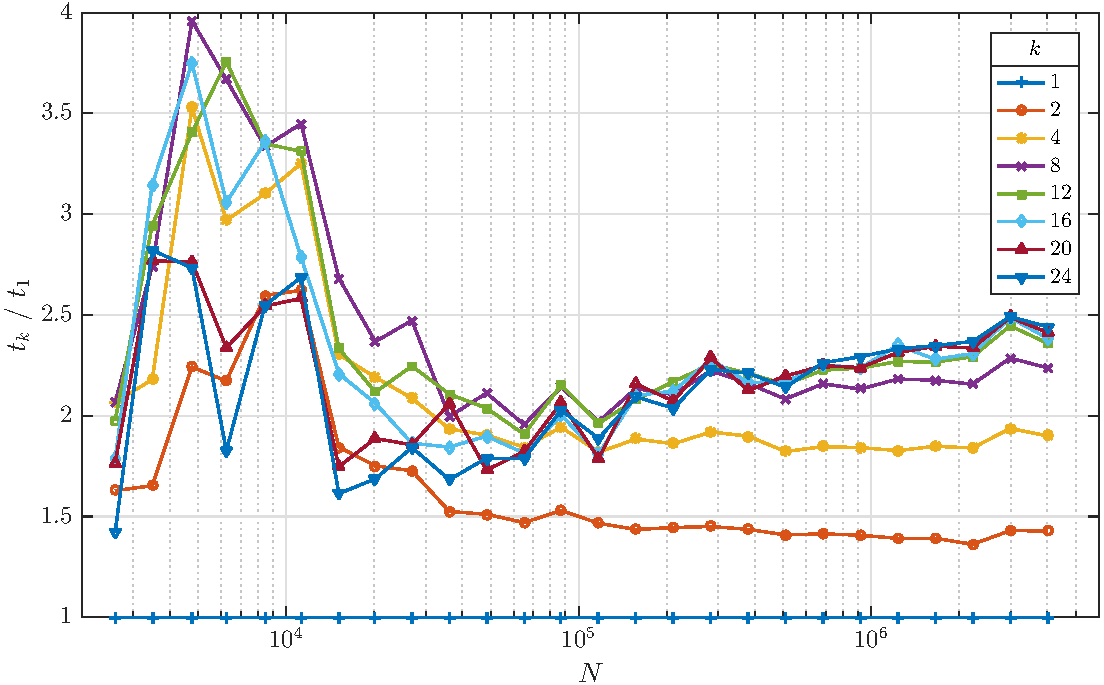
\includegraphics[width=\iw]{images/poisson_square_speedup.pdf}
  \caption[Faktorji pohitritve pri reševanju Poissonove enačbe.]{Faktorji pohitritve $f_k(N)$ pri
  reševanju problema~\eqref{eq:poisson-problem}.}
  \label{fig:poisson-square-speedup}
\end{figure}
Pri problemih z $N < 5\cdot 10^4$ se program že brez paralelizacije izvede v manj kot sekundi, tako
da so meritve pohitritve bolj nezanesljive in sama pohitritev ni tako pomembna, zato glejmo graf za
večje $N$. Vidimo, da se izvajanje pohitri, toda ne zelo, z asimptotičnim faktorjem pospešitve malo manj kot
1.5 za dve jedri, okoli 1.8 za štiri jedra in končnim faktorjem malo pod 2.5 za 12 jeder in več.
Zanimivo si je tudi ogledati novo razporeditev časov izvajanja posameznih kosov, prikazano za primer
$k =12$ na sliki~\ref{fig:poisson-square-time-distribution-12}.

\begin{figure}[!h]
  \centering
  \includegraphics[width=\iw]{images/poisson_square_time_distribution_12.pdf}
  \caption[Čas izvajanja delov programa pri uporabi 12 niti.]{Čas izvajanja posameznih delov programa pri reševanju
  problema~\eqref{eq:poisson-problem} z 12 nitmi.}
  \label{fig:poisson-square-time-distribution-12}
\end{figure}

Pričakovano se poveča delež, ki ga porabimo za grajenje domene, relativno pa se precej poveča delež
časa, ki ga porabimo za razcep matrike, saj se ta paralelizira slabše kot grajenje funkcij oblike.
Iz grafov na slikah~\ref{fig:poisson-square-time-distribution}
in~\ref{fig:poisson-square-time-distribution-12} preberemo, da je faktor pohitritve samo za funkcije
oblike približno $6.4$ za razcep matrike pa $1.7$.

Kljub slabim faktorjem pohitritve pri paralelizaciji, ta še vedno vsaj dvakrat skrajša čas izvajanja,
brez veliko truda ali sprememb v izvorni kodi, tako da ni razloga, da je ne bi uporabili.

\section{Zaključek}

V magistrskem delu smo si ogledali klasično teorijo elastomehanike in izpeljali Navierovo enačbo, ki
opisuje deformacijo teles pod zunanjimi obremenitvami. Pokazali smo obstoj in enoličnost šibkih
rešitev Navierove enačbe. Samega reševanja smo se lotili numerično in sicer s splošno MLSM metodo,
za katero smo pokazali, da v posebnih primerih preide v metodo končnih diferenc. Vpeljali smo tudi
algoritem za zgoščevanje in prilagajanje diskretizacije poljubnim oblikam ter demonstrirali njuno
uporabnost na več neregularnih domenah.

Metodo smo najprej testirali na preprosti Poissonovi enačbi, kjer smo analizirali obnašanje glede na
uporabo različnih baznih funkcij in uteži ter različnega števila sosedov. V nadaljevanju smo rešili
dva klasična primera iz elastostatike in sicer vpet nosilec ter Hertzev kontakt. Splošnost MLSM
glede postavitve diskretizacijskih točk smo predstavili preko rešitve navrtanega vpetega
nosilca, kjer smo morali opisati neregularno domeno ter zgostiti točke v okolici lukenj. Za konec
smo rešili še primer iz mehanike utrujanja materialov in pokazali ujemanje metode z referenčno
rešitvijo.

Nadaljnje delo bo usmerjeno v razvoj rešitvenega postopka za simulacijo rasti razpoke. V ta namen
bomo MLSM obogatili z adaptacijo baznih funkcij, kar bomo potrebovali za opis konice razpoke. Za
opis razpoke bomo prav tako potrebovali cenilko napake rešitve, saj ne bo več v naprej znano, kje
lahko pričakujemo največje napake. Pri računanju funkcij oblike bomo problem v posebnih, a pogostih
primerih, zastavili preko reševanja sistema in tako pridobili na času reševanja, ki bo pri
simulacijah rasti razpoke postal pomemben faktor. V ta namen se bomo posvetili tudi implementaciji
paralelnih rešitvenih postopkov, tako na arhitekturah s skupnim pomnilnikom, kot tudi na
distribuiranih arhitekturah.

%orabnik na voljo izbiro postopka za reševanje
%zastavimo preko reševanja sistema in tako pridobimo na času reševanja, hkrati pa odpremo večjo
%splošnost, saj ima uporabnik na voljo izbiro postopka za reševanje.

% Metodo samo se lahko obogati z večjo
% podporo za
%različne domene ali celo poveže s kakšnim sistemom za računsko podprto geometrijsko oblikovanje.
%Pri goščenju mreže se lahko poglobimo v različne cenilke napake rešitve, tako da bi avtomatsko
%vedeli, kje gostiti mrežo. Pri računanju funkcij oblike lahko problem v posebnih, a pogostih primerih
%zastavimo preko reševanja sistema in tako pridobimo na času reševanja, hkrati pa odpremo večjo
%splošnost, saj ima uporabnik na voljo izbiro postopka za reševanje.
%Na področju implementacije se
%lahko usmerimo v večjo modularno in razširimo nabor možnih aproksimacij ali pa v paralelizacijo
%postopka.

%Na področju mehanike materialov metoda še bolj pokaže svoje prednosti, ko se spustimo v simulacijo
%razpok, saj je potrebno domeno premikati in gostiti okoli vrha razpoke, vendar je potrebno njeno
%obnašanje še raziskati.

\cleardoublepage
\phantomsection
\addcontentsline{toc}{section}{Literatura}
\bibliographystyle{fmf-sl-num}
\bibliography{literatura}

\end{document}

% vim: set spell spelllang=sl:
